\documentclass[12pt,a4paper]{book}
\usepackage[utf8]{inputenc}
\usepackage[T1]{fontenc}
\usepackage[english]{babel}
\usepackage{graphicx}
\usepackage[authoryear,round]{natbib}
\bibliographystyle{unsrtnat}
\usepackage{xcolor}
\usepackage{booktabs} 
\usepackage{amsmath}
\usepackage{lscape}
\usepackage[left=2.5cm,right=2cm,top=2cm,bottom=1.7cm,includefoot,includehead,headheight=16pt]{geometry}
\usepackage{siunitx}
\setlength{\topmargin}{-1cm}
\setlength{\textheight}{24cm}
\setlength{\linewidth}{3cm}
% Estilo
\usepackage{amsmath,amssymb,amsfonts,stackrel,hyperref}
% \numberwithin{equation}{section}
\usepackage{graphicx,color}
\definecolor{verde}{RGB}{0, 83, 62}
\usepackage{setspace}
\renewcommand{\baselinestretch}{1.2}


% Tablas
\usepackage{tabularx,multirow,rotating,longtable}

% Código
\usepackage{listings} 
\usepackage[mathscr]{euscript}
\lstdefinestyle{estiloMUICD}{
    backgroundcolor=\color{black!5!white},
    commentstyle=\color{green!60!black},
    keywordstyle=\color{blue},
    numberstyle=\footnotesize,
    stringstyle=\color{black!40!white}\ttfamily,
    basicstyle=\small\ttfamily,
    breakatwhitespace=false,
    breaklines=true,
    captionpos=b,
    keepspaces=true,
    numbers=left,
    numbersep=8pt,
    showspaces=false,
    showstringspaces=false,
    showtabs=false,
    tabsize=2
}
\lstset{style=estiloMUICD}

% Tikz
\usepackage{tikz}
\usetikzlibrary{arrows}

% Encabezados
\usepackage{fancyhdr}
\fancyhf{}
\fancyhead{}
\pagestyle{fancy}
\fancyhead[LE,RO]{\thepage}
\fancyhead[LO, RE]{\leftmark}
\renewcommand{\chaptermark}[1]{\markboth{#1}{}}
\renewcommand{\chaptermark}[1]{\markright{#1}}
\pagestyle{empty}

% Glosarios y nomenclaturas
\usepackage[toc,nonumberlist]{glossaries}


\title{Thesis}
\author{sebastian.perezvasseur}
\date{January 2025}

\begin{document}
\newcommand{\no}{NO$_{2}$}
\newcommand{\ot}{O$_{3}$}
\newcommand{\pmtwo}{PM$_{2.5}$}
\newcommand{\pmten}{PM$_{10}$}

\frontmatter
\begin{titlepage}
\centering
	
\includegraphics[height=4cm]{logo_informatica_s.png}\\
	\vspace{0.25cm}
 	{\Large \textsc{{Universidad Nacional\\ de Educación a Distancia}}}\\
 	\vspace{0.8cm}
	{\Large Escuela Técnica Superior de Ingeniería Informática}\\
	\vspace{0.25cm}
	\vspace{1.5cm}
    \begin{spacing}{2}
 	{\textsc{\Huge Probabilistic Forecast of air quality in the city of Madrid}}
    \end{spacing}
	\vfill
	{\Large Sebastien Perez Vasseur}\\
	\vspace{0.3cm}
	\begin{tabular}{ll}
	% Sustituir [Director] por el nombre del director
	\large Director/a: & \large Jose L. Aznarte\\
	\vspace{0.3cm}
	\large Co-director/a: & \large Javier Olivares
	\end{tabular}
	
	\vfill
	{\Large Memoria de Doctorado}\\
	\vspace{0.3cm}
	{\large Doctorado\\ en Sistemas Inteligentes}\\
	\vspace{0.25cm}
	Septiembre de 2025
\end{titlepage}
\cleardoublepage{}

\tableofcontents
\listoffigures
\renewcommand{\listtablename}{List of tables}
\listoftables

\mainmatter

\chapter{Introduction}

%Pollution as an issue%
Urban pollution is a concern in metropolitan areas due to its detrimental effects on public health and environmental impact. The origins of air pollution can be traced to several human-driven activities, including emissions from vehicles, power plants, and off-road machinery, all of which contribute to serious environmental and health problems. Pollutants such as particulate matter (PM), ozone (\ot), and nitrogen dioxide (\no) are associated with significant health risks, including cardiovascular diseases \citep{lee_air_2014}, respiratory disorders \citep{kurt_pulmonary_2016}, diabetes \citep{eze_long-term_2014}, chronic kidney disease \citep{bowe_particulate_2018}, increased mortality \citep{tang_mortality_2017}, and neurological impairments \citep{lee_traffic-related_2016}. While \citet{landrigan_pollution_2018} offer a comprehensive overview of the health conditions linked to various forms of pollution, \citet{NAVARES2020109254} also shows that there's a direct correlation between pollution and rising hospital admissions.

Consequently, major urban centers with degraded air quality like the city of Madrid \citep{gonzalez-garcia_environmental_2021} face serious health challenges \citep{aguilar_relationship_2021}, which underlines the necessity for mitigation strategies.

In light of this, cities such as Barcelona \citep{barcelonamesaure} and New Delhi \citep{newdelhimeasure} have set emergency plans to control the impact of air pollution. Moreover, other cities like Madrid have more advanced efforts by implementing sophisticated air quality forecasting systems designed to detect pollution events and activate contingency protocols. In Madrid, the SOCAIRE forecasting system \citep{de_medrano_socaire_2021} provides forecasts of surges in the concentration of the \no{} pollutant and triggers preventive measures, such as reducing vehicule traffic. Because these interventions have a non-neglegible economic impact \citep{madrid_protocolo_no}, they highlight the need of generating accurate and confident forecasts.

%Machine learning as a field to provide forecast%
Therefore, we focus on the latest innovations in pollution forecasting and also in the more general time series forecasting field. In this last field, we see how Machine Learning (ML) has emerged as the most reliable set of methods, outperforming conventional statistical approaches. We have witnessed this in the MX competitions \citep[e.g. ][]{makridakis_m3-competition:_2000,makridakis_m4_2020,makridakis_m5_2022}, organized as a benchmark of different time series forecasting methods. Historically, statistical methods were outperforming machine learning methods until recently. First, we saw hybrid models, blending statistical methods and ML techniques winning the competition. Then in the last competition, full ML methods are getting the upper hand with models like LightGBM \citep{NIPS2017_6449f44a}, which is a gradient boost based method.

%Neural Networks and Global Forecasting models%
Contemporary research has also further advanced the field of time series forecast by applying innovative deep learning architectures, such as Convolutional Neural Networks (CONV) \citep{lecun_convolutional_1998}, Long Short-Term Memory networks (LSTMs) \citep{lstmhochreiter1997long}, and transformers \citep{transvaswani_attention_2023}, to time series forecasting. Recent studies \citep{masood_review_2021} indicate that these architectures can yield promising results. Also, another effective strategy to boost the model's performance is to expand the available training data. In this context, global forecasting models (GFMs), which learn concurrently from multiple related time series rather than isolated instances, produce superior outcomes, as demonstrated in the work of Hewamalage et al. \citep{hewamalage_advancing_2022}. In light of these advances, it is both interesting and timely to \textbf{explore the integration of global forecasting models with cutting-edge architectures like LSTM or transformers}. 

%Uncertainty Presentation%
As stated previously, we need accurate and confident forecasts, and the uncertainty of the forecast is linked to the confidence of the predictions. This uncertainty needs to be described and formalized, and we found that probabilistic forecasting is a first step towards quantifying it. Indeed, unlike single-point forecasting, probabilistic forecasting presents a distribution of future outcomes. This distributional approach allows to capture the uncertainty of the forecast as it presents the range and likelihood of potential outcomes. The dispersion of the predicted target distribution indicates the model’s confidence in its forecast. A wider spread, indicated for example by a higher standard deviation, suggests a greater variety of plausible values, reflecting higher uncertainty or lower confidence in the prediction. Conversely, a narrower distribution implies a tighter clustering of forecasted outcomes, denoting higher confidence or lower uncertainty. Thus, the forecast's uncertainty provides critical information required for comprehensive decision making. As a result, probabilistic forecasting models, which offer a full distribution of potential outcomes are increasingly preferred. This shift is underscored for example by the inclusion of an “uncertainty” category in the M5 competition, highlighting the importance of quantifying and communicating prediction uncertainty, which is essential for informed decision-making in fields such as environmental management.

%Visualization of results%
Finally, there is a clear opportunity to support analysts who struggle with the abstract nature of probability and the limitations of current visualization methods. Despite recent innovations in uncertainty visualization, their application to time series data remains limited. Consequently, developing a novel visualization framework specifically for time series uncertainty, validated through user testing, could significantly enhance the interpretability of complex models. This approach would not only facilitate a deeper understanding of the underlying processes driving forecasts but also improve overall model accuracy through greater practitioner engagement during model training.

%Structure of the thesis%
To analyze and improve current methods for air pollution probabilistic forecasting and the visualization of its results, this work is structured as follows. Chapter 2 provides a critical review of the state of probabilistic forecast of air pollution. It lists the latest techniques, describes the principal methods, explains the principles of global forecasting, and discusses uncertainty in forecasting models, covering both inference methods and the current methods to visualize that uncertainty. Chapter 3 outlines our proposed innovative models. In chapter 4, we detail the experimental setup used to compare these models, including the data description, pre-processing steps, and evaluation metrics. Chapter 5 then presents the results and offers insight into improving air pollution forecasting. Chapter 6 concludes with our findings and perspectives on future research. Finally, we add a section in the annex with an experiment aiming at improving the visualization of probabilistic predictions.

\chapter{State of the art}
\section{Air quality forecasting}
%Physics Model%
Recent advances in both physics-based models and machine learning techniques are significantly improving the field of air quality forecasting. Eulerian, Lagrangian, dispersion, chemical transport, and meteorological simulations represent the main methods based on physics. In eulerian models, such as those described by \citet{wong_wrf-cmaq_2012}, the atmosphere is divided into a grid and the fluid dynamics across different cells is analyzed. However, in Lagrangian models, referenced by \citet{eliassen_aspects_1984} and \citet{romanov_graz_2020}, air parcels are tracked as they move through the atmosphere. Chemical Transport Models (CTM) analyze fluid dynamics and chemical reactions in the air: examples are WRF-Chem \citep{georgiou_evaluation_2022}, AURAMS \citep{smyth_comparative_2009}, CHIMERE \citep{menut_chimere_2021}, and COSMO-ART \citep{ponomarev_application_2020}. Finally, meteorological models \citep{liu_air_2022} predict air pollution levels by simulating weather patterns. Due to their computational cost, these physics-based models often feature a relatively low resolution. Since they simulate complex atmospheric processes on a continental scale, the available data is often restricted to large-scale observations, limiting their precision at finer spatial levels.

%Statistical models%
Physics-based models help understanding air pollution dynamics and offer a sound approach to simulate atmospheric conditions. However, they are computationally intensive and difficult to calibrate, as highlighted by \citet{gardner-frolick_selecting_2022}. Another major drawback is their low resolution, which limits their usefulness in making local air quality predictions at city level.

On the other hand, research on statistical and machine learning approaches for air quality forecasting \citep[e.g. ][]{bai_air_2018,masood_review_2021} help addressing those issues. Traditional statistical methods include linear regression and ARIMA \citep{diaz-robles_hybrid_2008}, as well as ARIMA-based techniques like SARIMAX \citep{de_medrano_socaire_2021}. In the field of machine learning, various models have been explored such as support vector regression \citep{garcia_nieto_svm-based_2013,yeganeh_prediction_2012}, fuzzy logic \citep{carbajal-hernandez_assessment_2012}, random forests \citep{thongthammachart_integrated_2021}, and gradient boosting \citep{ma_time_2022}. Furthermore, deep learning techniques such as multi-layer perceptrons \citep{singh_linear_2012}, long short-term memory networks (LSTM) \citep{alhirmizy_multivariate_2019}, and convolutional neural networks (CNN) \citep{soh_adaptive_2018} have also been applied.

%Machine learning%
As noted by \citet{gardner-frolick_selecting_2022}, the machine learning approaches have issues of interpretability as they do not always offer an easy way to understand how the predictions were calculated. It is true that intensive research is being done on interpreting the predictions of those models \citep{vega_garcia_shapley_2020}, but those methods still face significant challenges and are not yet mature enough for widespread, uncritical adoption \citep{Silva2024, rudin_stop_2019}. Also, due to the nature of machine learning, predictions can only be based on past training data and therefore it might present issues with new out-of-sample situations. The rise of hybrid approaches incorporates the best of both worlds with machine learning models using the predictions of physics model as input \citep[e.g. ][]{de_medrano_socaire_2021} or machine learning models guided by physics knowledge \citep[e.g. ][]{hettige_airphynet:_2024}.

In order to compare time series forecasting techniques, the MX competitions \citep[e.g. ][]{makridakis_m3-competition:_2000,makridakis_m4_2020,makridakis_m5_2022} were organized where different architectures compete against each other by forecasting a set of time series. During those competitions, statistical methods have outperformed machine learning methods until recently. Gradient boost methods and specially LightGBM \citep{NIPS2017_6449f44a} methods changed this situation. LightGBM features a series of innovations that not only make it more efficient but also provide better results. For example, instead of growing trees level-wise, LightGBM focuses on the leaves that provide the maximum reduction in loss, which achieves better accuracy. Also their histogram-based algorithms reduce the computational cost by categorizing continuous feature values into discrete bins.

\citet{masood_review_2021} identify deep neural networks (DNNs) such as LSTM or CNN as the best performing machine learning based techniques for air pollution forecasting. This conclusion is based on the results of a performance analysis demonstrating that DNNs have the the best overall root mean squared error (RMSE) compared to other AI-based techniques for air pollution forecasting. The superior performance of DNNs is attributed to their deep architecture, which enables them to extract more complex features from the input data, leading to more accurate results.

\section{Main time series forecasting models}
The following subsection provide an overview of several fundamental machine learning models, from classical machine learning models like linear regression, K nearest neighbor, gradient boosting or random forest to complex deep learning architectures like long-short term memory networks, convolutional neural networks or Transformers.

%Linear regression%
Linear regression \citep{montgomery2012lrintroduction} is a popular choice due to its simplicity and ease of understanding. On training, the model calculates the linear coefficients between the input variable and the target variable. The model’s coefficients show directly how each input affects the output, making it easy to understand the relationships between variables. This is useful in fields like finance, healthcare, and social sciences, where clear explanations are necessary. 

%KNeighbors%

The K-Nearest Neighbors (KNN) \citep{knnaltman_introduction_1992} machine learning method predicts the value of a new data point by considering the closest K neighbors in the feature space. It calculates distances (often using Euclidean distance, but other metrics like Manhattan or Minkowski can be used) between the query point and training samples, then averages the values of the K nearest neighbors. This method is simple yet effective, especially in low-dimensional spaces.

%Gradient Boost%
Gradient Boosting \citep{gradientfriedman_greedy_2001} is an ensemble machine learning method which builds models sequentially by predicting the errors of previous models and adjusting based on it. Simpler models are fitted to the residual errors of the previous ones and a new prediction is built on top of those past predictions. The algorithm minimizes a chosen loss function using gradient descent, adjusting predictions iteratively to improve accuracy. This method is highly accurate, but it can be prone to overfitting if not properly regularized. Popular implementations include XGBoost \citep{xgboostchen_xgboost:_2016}, LightGBM \citep{lightgbmke_lightgbm:_2017}, and CatBoost \citep{catboostprokhorenkova_catboost:_2018}.

%Random Forest%

Random Forest \citep{breiman_random_2001} is an ensemble learning method that combines multiple decision trees. It works by training each tree on a random subset of the data (using bootstrap sampling) with a random subset of features at each split. Predictions are made by averaging outputs across all trees. This method is highly effective, handles large datasets well, and is resistant to noise, but it can be computationally expensive and less interpretable than individual decision trees.

%MLP%
A Multi-Layer Perceptron (MLP) \citep{mlprumelhart_learning_1986} is a type of artificial neural network composed of multiple layers of neurons, including an input layer, one or more hidden layers, and an output layer. Each neuron in one layer is fully connected to every neuron in the next layer, and they use activation functions like ReLU or sigmoid to introduce non-linearity. 

%LSTM%
\label{lstm}
Long Short-Term Memory (LSTM) \citep{lstmhochreiter1997long} is a type of recurrent neural network (RNN) designed to handle sequential data and capture long-range dependencies while addressing the vanishing gradient problem. LSTMs use a unique memory cell structure with three gates: input gate, forget gate, and output gate. These gates enable LSTMs to retain relevant information over long time steps, making them highly effective for tasks like time-series forecasting, speech recognition, and natural language processing (NLP). However, they can be computationally expensive compared to simpler models.

%CNN%
A Convolutional Neural Network (CNN) \citep{lecun_convolutional_1995}, a type of deep learning model, consists of multiple layers, including convolutional layers, which apply filters to detect patterns like edges and textures; pooling layers, which reduce the spatial dimensions to retain important features while minimizing computation; and fully connected layers, which interpret these extracted features for classification or other tasks. CNNs excel in image recognition, object detection, and computer vision applications due to their ability to learn spatial or time hierarchies.

%Transformers%
Transformers \citep{transvaswani_attention_2023} are a deep learning architecture designed for handling sequential data, particularly excelling in natural language processing (NLP) tasks. Unlike traditional recurrent neural networks (RNNs), transformers rely on self-attention mechanisms to process entire input sequences simultaneously, capturing long-range dependencies more effectively. The key components include multi-head self-attention, which enables the model to focus on different parts of the input simultaneously, and positional encoding, which retains the order of tokens despite the lack of recurrence. Transformers power state-of-the-art models like BERT, GPT, and T5, and they have also been adapted for vision tasks (ViTs). Their efficiency in parallel computation and ability to model complex relationships make them dominant in modern AI applications.

\section{Global Forecasting Models}
%Literature on GFM from article 3%
\citet{januschowski_criteria_2020} introduce the concept of Global Forecasting Models (GFMs). Those are different from local models in that they are trained on an entire dataset of time series rather than on a single time series. Therefore, a single GFM can generate forecasts for any time series within the training dataset. As noted by \citet{hewamalage_recurrent_2021}, GFMs outperform their local counterpart, thanks to their ability to leverage a larger volume of data and capture cross-series dependencies, which enhances predictive performance.

Further research by \citet{hewamalage_advancing_2022} demonstrates the superiority of GFMs over traditional statistical methods, which by definition are local. Specifically, deep neural networks trained as GFMs outperform methods such as ARIMA and exponential smoothing across multiple forecasting scenarios, including the M3 competition dataset. Moreover, \citet{bandara_forecasting_2020} find that the effectiveness of GFMs increases when the time series within the training set exhibit similar characteristics. Clustering techniques can therefore be employed to group similar time series, further enhancing forecast accuracy.

Despite these advancements, the application of GFMs in air quality forecasting remains underexplored. Given that air quality forecasting relies on numerous related time series from different monitoring stations and various pollutants, GFMs present significant potential for improving predictive accuracy in this domain.

In the case of air quality forecasting, GFMs remain largely unexplored and offer a lot of potential. Indeed, air quality forecasting uses as input many similar (and highly correlated) time series from different air quality stations and for different chemicals or particulate matters.

\section{Uncertainty in models}
%Literature on GFM from article 3%
\citet{cabaneros_methods_2022} describes the uncertainty sources in air quality forecasting: input uncertainty, structure uncertainty, parameter uncertainty and output uncertainty. Input uncertainty is a direct consequence of the training data. First, selecting predictors from air pollutants, meteorological or temporal variables requires searching a vast array of possibilities (all subseets of variable combinations). Most methods are not exhaustive and randomly explore that space, which means the solution can vary on each execution. Also, we are limited by the sample in the training data (data density) which is not the complete space of the predictor space. For example, pollution peaks are a rare event and is more uncertain to predict as we have less data available on them. Finally, error rate in the sensors (\citep{peters_evaluating_2022, gerboles_estimation_2010}) or missing values introduce gaps and uncertainty in the data. Finding the correct machine learning architecture and hyperparameters is also a search in a vast space of possibilities. There is no clear, one-size-fits-all rule for building the best forecasting model, leading to trial-and-error in deciding the model's architecture. Same thing happens with the hyperparameters of the model. This creates uncertainty as the search algorithm is not guaranteed to lead to the optimum of its cost function. 

The model's output uncertainty arises from the inputs, model design, and parameters choice. However, single-point forecasting methods do not take into account these uncertainties. And actually, running the exact same experiment might lead to different results because this uncertainty has not been considered. This should be considered, even if the uncertainty is not considerable. Probabilistic forecasting does address this and describes the uncertainty in the forecasts. 

\section{Uncertainty inference methods}
There are different ways to describe the probability distribution of the data such as quantile ranges \cite{chen_evaluating_2022}, parameters of a known distribution (e.g., normal, Beta, ...) \cite{fernandez-jimenez_short-term_2023}, generic parameters like location, scale or shape \citep{marz_xgboostlss_2019} or transformation parameters for a standard distribution like Gaussian into the target distribution \citep{rasul2021multivariate}.

\subsection{Parametric}
%Parametric%
This technique \cite{fernandez-jimenez_short-term_2023} involves assuming beforehand that the target variable belongs to a specific, known probability distribution—such as the Normal, Beta ... and estimating its parameters directly from the data. This approach integrates domain specific knowledge as the choice of the distribution depends on an analysis of the target variable. 
Then instead of predicting the whole shape of the distribution, we only need to predict a low number of parameters like the mean and the standard deviation for a normal distribution.
The prediction then involves calculating the distribution from the predicted parameters.

This parametric approach results in models that are straightforward to implement and understand. The compact representation using a few parameters also simplifies the integration of domain-specific knowledge into the forecasting framework. However, if the chosen distribution does not accurately represent the underlying data, the resulting forecasts is misleading. This risk of using the wrong model can limit the method's applicability, particularly in real-world scenarios where data may exhibit features (e.g., skewness, kurtosis) that deviate from standard distributions. Finally, many variables can not be modeled with a known distribution.

%Quantile%
\subsection{Quantile range}
\label{status:quantile}
Usually, point forecasting focuses on the prediction $\hat y(x)$ which minimizes the mean squared error,
\begin{equation}
  \label{eq:1}
  E = \frac{1}{n} \sum^n_i \epsilon_i =
  \frac{1}{n} \sum^n_i [ y_i - \hat y(x)]^2.
\end{equation}

This prediction is the conditional sample mean of $y$ given $x$ or the location of the conditional distribution. But we could be interested in estimating the conditional median (i.e., the 0.5 quantile) instead of the mean, in which case we should find the prediction $\hat y(x)$ which minimizes the mean absolute error,
\begin{equation}
  \label{eq:2}
  E = \frac{1}{n} \sum^n_i \epsilon_i =
  \frac{1}{n} \sum^n_i | y_i - \hat y(x) |.
\end{equation}

The fact is that, apart from the 0.5 quantile, it is possible to estimate any other given quantile $\tau$. In that case, instead of (\ref{eq:2}), we could minimize
\begin{equation}
  \label{eq:3}
  E= \frac{1}{n} \sum^n_i f( y_i - \hat y(x))
\end{equation}
where
\begin{equation}
  \label{eq:4}
  f(y-q) = \left\{ 
    \begin{array}{l l}
      \tau (y-q) & \quad \mbox{if $y \ge q$}\\
      (1-\tau) (q-y) & \quad \mbox{if $y < q$}\\
    \end{array} \right.,
\end{equation}

with $\tau \in (0,1)$. Equation (\ref{eq:3}) represents the median when $\tau=0.5$ and the $\tau$-th quantile in any other case.

Quantile ranges allow for a direct estimation of prediction intervals without relying on strict assumptions. This means the prediction is highly adaptable to any distribution.
Also, they offer an intuitive interpretation of the uncertainty as they show a range of possible future observations. However, estimating multiple quantiles can become computationally demanding, particularly if there's a need for a complete distribution description. Quantile crossing is also problematic, where estimated quantiles do not maintain the required order, requiring additional constraints or post-processing. Finally, parametric estimation is preferred when the chosen distribution fits well the target variable.

\subsection{Location, Scale and Shape}
%LSS%
The LSS approach \citep{marz_xgboostlss_2019} uses generic parameters like location, scale, and shape to model the underlying distribution. This does not require prior domain-specific knowledge and can adapt in case of distribution heterogeneity. One of the main models using this technique is XGBoostLSS. However, this method requires higher amount of data since the estimates can become unstable. Indeed, different combinations of parameter values could lead to nearly identical model outputs, which could create noticeable differences in predictions on near timeframes. Additionally, it's difficult to interpret the results as shape parameters are abstract.

\subsection{Flow}
%Flow%
Normalizing flows are generative models that employ invertible transformations to map simple base distributions like Gaussian to complex target distributions. This technique has been successfully applied in time series forecasting \citep{flowtimerasul_multivariate_2021}, image \citep{imagetan_flowvqtalker:_2024} and audio generation \citep{flowaudiobilinski_creating_2023}. In time series forecasting, a conditioned normalizing flow (conditioned on the previous values) could be implemented to forecast the future values. Then, this method could enhance uncertainty representation because it can model complex, real-world distributions without being constrained by the rigid assumptions of traditional parametric models. The transformation could go to from a simple skewness and kurtosis transformation to more complex transformations involving several steps. However, the more complex the transformation the more parameters it would have. Also, we need to ensure the invertability of the transformation which adds additional constraints.  Additionally, as this transformation involves a high number of parameters, we could face issues like  overfitting or low stability over time (a sequence of very different parameters). Finally, the models does not offer easy interpretability as it is not directly predicting the distribution. 

\subsection{Diffusion}
%Diffusion%
Diffusion models \citep{diftimemeijer_rise_2024} are generative models that learn to gradually denoise data. In the diffusion process, data is first transformed into noise by adding noise through a series of small steps (the forward process). Then, a neural network is trained to reverse this process (the reverse denoising process), also step by step, to recover the original data distribution. In time series forecasting, the denoising model is conditioned on observed historical values, and then diffusion process is used to generate future values. Because the model learns to approximate the true data distribution, it can generate forecasts that are a better fit to that distribution. Recent implementations \citep{diftimemeijer_rise_2024} have demonstrated competitive or even superior performance compared to traditional forecasting models. However, this technique has some disadvantages. First, diffusion models typically require a large number of iterative denoising steps to produce a single forecast. This makes training and especially inference computationally expensive and slower compared to more direct forecasting methods. Also, the process involves multiple design choices (for example, the noise schedule, number of steps) that can be sensitive to tuning. This complexity can make the model harder to deploy and optimize in practice.

\chapter{Proposed Models for probabilistic pollution forecasting} 
\label{sec:proposemodel}
This section describes the different models proposed to advance the field of probabilistic time series forecasting for air quality. Those models are compared in 2 different sets of experiments. The first group of models are classical machine learning models, whose main characteristic is that they do not take into account the sequential nature of time series. They use as input tabular data with a variety of predictors such as the lagged values of the target variable but they do not extract patterns based on the order of those values. On the contrary, the second group of models, based on deep learning architectures, do learn from that order.

\section{\no{} Probability Distribution}
Upon analysis from a previous article \citep{vasseur_comparing_2021} (Figure \ref{figure:histo_variance}), we determine that the Gaussian distribution is a good approximation of the log transformed \no{} distribution. Consequently, we propose to design our forecasting models to output the parameters of such distribution: mean and standard deviation.

\section{Classical Machine Learning Models} 

%Article 1 models% 
\subsection{Quantile linear regression} 
\label{model:qlr}
A linear regression can be used to predict the 
quantiles of the target variable with the previously defined modified cost function in Section \ref{status:quantile}. Then to generate a full probabilistic forecast, we model the target variable's distribution as a Gaussian, defined by its mean ($\mu$) and standard deviation ($\sigma$). We estimate these parameters using quantile regression. Specifically, we train five independent linear regression models, each optimized with a modified cost function to predict the target variable's value at a key percentile. The chosen percentiles are 2.5\%, 16\%, 50\% (the median), 84\%, and 97.5\%. These were selected because they correspond to the median $\mu$, $\mu\pm\sigma$, and $\mu\pm2\sigma$ points of a normal distribution. From the five predicted quantile values, we can then directly calculate the distribution's final mean and standard deviation, providing a complete probabilistic forecast.

\subsection{Quantile k‑nearest neighbors} 
We use a probabilistic version of the k-nearest neighbors algorithm. This algorithm is based on the standard k nearest neighbor, where instead of calculating the mean of the target for the most similar observation points, we fit a Gaussian distribution on those points.

\subsection{Quantile random forests} 
A random forest is an ensemble learning method that combines multiple decision trees from bootstrap samples of the training data. In a standard regression random forest, each tree partitions the feature space into a set of regions using recursive binary splits. Hence, each leaf node in the decision tree contains a subset of the training data points in that region and their corresponding target values. The final prediction for a given input is computed as the average of those target values. The random forest then aggregates predictions from multiple trees by calculating the average of each tree prediction.

Instead of summarizing the leaf distribution with a single value (mean), we can represent the full distribution of target values within each leaf. This leads to a probabilistic decision tree, where each leaf node contains a histogram of the observed target values rather than a single summary statistic like the mean. Then the Quantile Random Forest (QRF) aggregates these empirical distributions across all trees, typically using a weighted combination. By doing this, QRF provides a full conditional distribution of the target variable given the input features, rather than just a single point estimate. Finally, we fit a Gaussian distribution to the predicted distribution by estimating the mean and variance of the aggregated distribution

\subsection{Quantile gradient boosted trees} 
\label{model:qgb}
To create quantile gradient boosted trees (QGB), we create 5 different models with different cost functions, each aimed at calculating a specific percentile ($\mu$, $\mu\pm\sigma$, and $\mu\pm2\sigma$). Then we calculate the parameters of a Gaussian distribution in the same way we did for the quantile linear regression (QLR), described previously \ref{model:qlr}. 

\subsection{Multilayer perceptron} 
We also consider a multilayer perceptron (MLP) with one hidden layer. As with quantile linear regression and quantile gradient boosted trees, we modify the cost function to predict specific quantiles of the target variable. To achieve this, we train five separate MLP models, each estimating a different percentile of the \no{} signal at $\mu$, $\mu\pm\sigma$, and $\mu\pm2\sigma$ points. Then we also calculate the parameters of a Gaussian distribution in the same way we did for the quantile linear regression (QLR), described previously \ref{model:qlr}.

\subsection{Distributional Forests} 
Distributional forests are a class of parametric probabilistic models which predict the parameters of the distribution of the target vairiable (in our case, a zero-censored Gaussian distribution). This model is based on the random forest idea, where multiple decision trees are constructed. Each tree partitions the training observation space and assigns those observations to leaf nodes. For a new input point z, the model collects observations from all leaves from all tress where z would fall. These observations are used to fit a zero-censored Gaussian distribution. However, rather than treating observations with simple integer counts (for example, using the number of times they appear together in a leaf), the model uses weighted maximum likelihood estimations. The weights are derived from how frequently each observation co-occurs with z in leaves across all trees, but are adjusted to account for leaf sizes and tree structure. This allows fractional and smooth weighting rather than abrupt count-based weighting. The reason for this design is to prevent over representation of observations from large leaves and to allow a stable, continuous estimate of distribution parameters.

\subsection{NGBoost} 
NGBoost is a probabilistic prediction model that employs a \textbf{parametric approach}. Indeed, it predicts the parameters of a Gaussian distribution — the mean ($\mu$) and the logarithm of the standard deviation ($\log(\sigma)$). The model is based on gradient boosting with decision trees, however unlike traditional gradient boosting methods that predict scalar values, it uses these iterations to refine predictions of distributional parameters. At each iteration, the model computes the gradient of the negative log-likelihood (NLL), which indicates how to adjust the parameters to achieve a better fit. NGBoost uses natural gradients to ensure that parameter updates are stable and appropriately sized. Indeed, directly applying ordinary gradients can result in overly large adjustments, especially for sensitive parameters like $\log(\sigma)$. It uses the Fisher Information Matrix ($I(\theta)$) to scale these gradients. This iterative process allows NGBoost to continuously refine its probabilistic predictions in a stable and controlled manner.

\subsection{Probabilistic forecast of linear regression residuals} 
We observe a strong linear dependency between the input predictors and the target variable, and therefore we propose combining three quantile-based models (Quantile Random Forest (QRF), Quantile k-Nearest Neighbors (QKNN), and Quantile Gradient Boosted Trees (QGB)) with a linear regression model. Specifically, we first train a linear regressor to predict the \no values and then train the QRF, QKNN, and QGB models to estimate the distribution of the residuals. We abbreviate both modelsrespectively with QRFL, QKNNL and QGBL.

\section{Deep learning based models} 

\subsection{Long short-term memory} 
%Modelo LSTM + MLP%
The LSTM architecture as described in Section \ref{lstm} do not produce probabilistic outputs, therefore we adapt them for this purpose and create a parametric model from this architecture. We use an LSTM encoder module where the input sequence is encoded into a feature vector. This vector is then passed to a multi-layer perceptron (MLP), which outputs the mean and variance of a Gaussian distribution.  

Although MLP models are widely used, there is limited research on the design of this architecture \citep{ramchoun_multilayer_2016,castro_multilayer_2017}. In particular, we did not find empirical rules to choose the depth or the number of nodes per layer. Some guidelines exist \cite{doug_answer_2012}, but they are not supported by rigorous research studies. Those suggests treating these design choices as an optimization problem where those are considered as parameters. In addition, since our MLP output two parameters, we could consider either a single MLP for a joint output or two separate MLPs, one for the mean and another one for the variance. In the absence of recommendations, we tested all configurations: number of MLPs, depth, and number of nodes.

\subsection{Convolutional Neural Network} 
%Modelo CNN + MLP%
Similarly, we propose integrating a convolutional neural network (CNN) with an MLP. The CNN processes the input sequence and transforms it into multiple output sequences, each capturing distinct patterns in the original data. Then an MLP estimate the parameters of the target distribution from those sequences. As in the previous section, we also test various MLP architectures in this setup, varying the depth, width and number of MLPs.

\subsection{Transformers} 
%Transformer%
We build a similar architecture with a transformer encoder module to extract rich representations from the input sequences. These encoded features are used as input for predicting the parameters of the Gaussian distribution of the target variable, specifically the mean and variance. As previously, we experiment with different configurations, varying the depth, width, and number of MLPs.

\chapter{Experimental Design}
\section{Overall philosophy}
This study aims to identify the optimal machine learning architecture for predicting \no{} levels. We evaluate and compare the proposed library of models split in two categories: classical machine learning algorithms and the more advanced deep learning architectures.

In the classical set of methods, we adapt those models for probabilistic forecasting as described in section \ref{sec:proposemodel}. Then after training the models, we forecast on one of the station every hour on a 60h range in the future in one of the stations in Madrid (Escuelas Aguirre). Then we evaluate the performance of the models through a predefined set of metrics which are detailed in the subsequent section. In this set of experiments, we have a semi-parametric approach where we are building the parameters of the distribution from quantile predictions.

In the deep learning set of experiments, we adapt again the models to be probabilistic and this time we forecast only on the 13h horizon, but on all 25 stations in Madrid. Not only do we introduce more advanced models, but we also improve the pre-processing step of the data prior to training and we test the impact on performance with different types of input training data. First, we test the performance gains from training the models as global forecasting models (GFM) and secondly we also compare the performance of univariate vs multivariate models. In order to build the probabilistic forecasts, we predict the parameters of the probability distribution of the target variable (\no{} levels in $\mu g/m^3$).  Indeed as the air quality protocol is triggered by the concentration of \no{} values \cite{madrid_protocolo_no}, we are only interested in the values of this indicator. The metrics of this experiment are defined in a subsequent section and are centered around evaluating the 50th quantile and overall fit of the forecasted probability distribution. Also, note that we are only evaluating the forecasted \no{} probability distribution. This is in contrast with other global forecasting approaches that measure the accuracy of their models across all the time series used \citep[e.g.,][]{hewamalage_advancing_2022,makridakis_m5_2022}. Thus, for each experimental configuration, we train with several time series but only forecast the \no{} level at the 13h horizon.

Finally, we execute a final set of experiments aimed at calibrating and evaluating the models with post-hoc calibration methods. We calibrate the best models from the previous experiment with a set of methods as defined in a subsequent section \ref{exp:posthoc} and we evaluate those calibration methods with the same metrics. Our objective is to understand the potential benefits of calibrating the machine learning methods. 

\begin{figure}
  \centering
  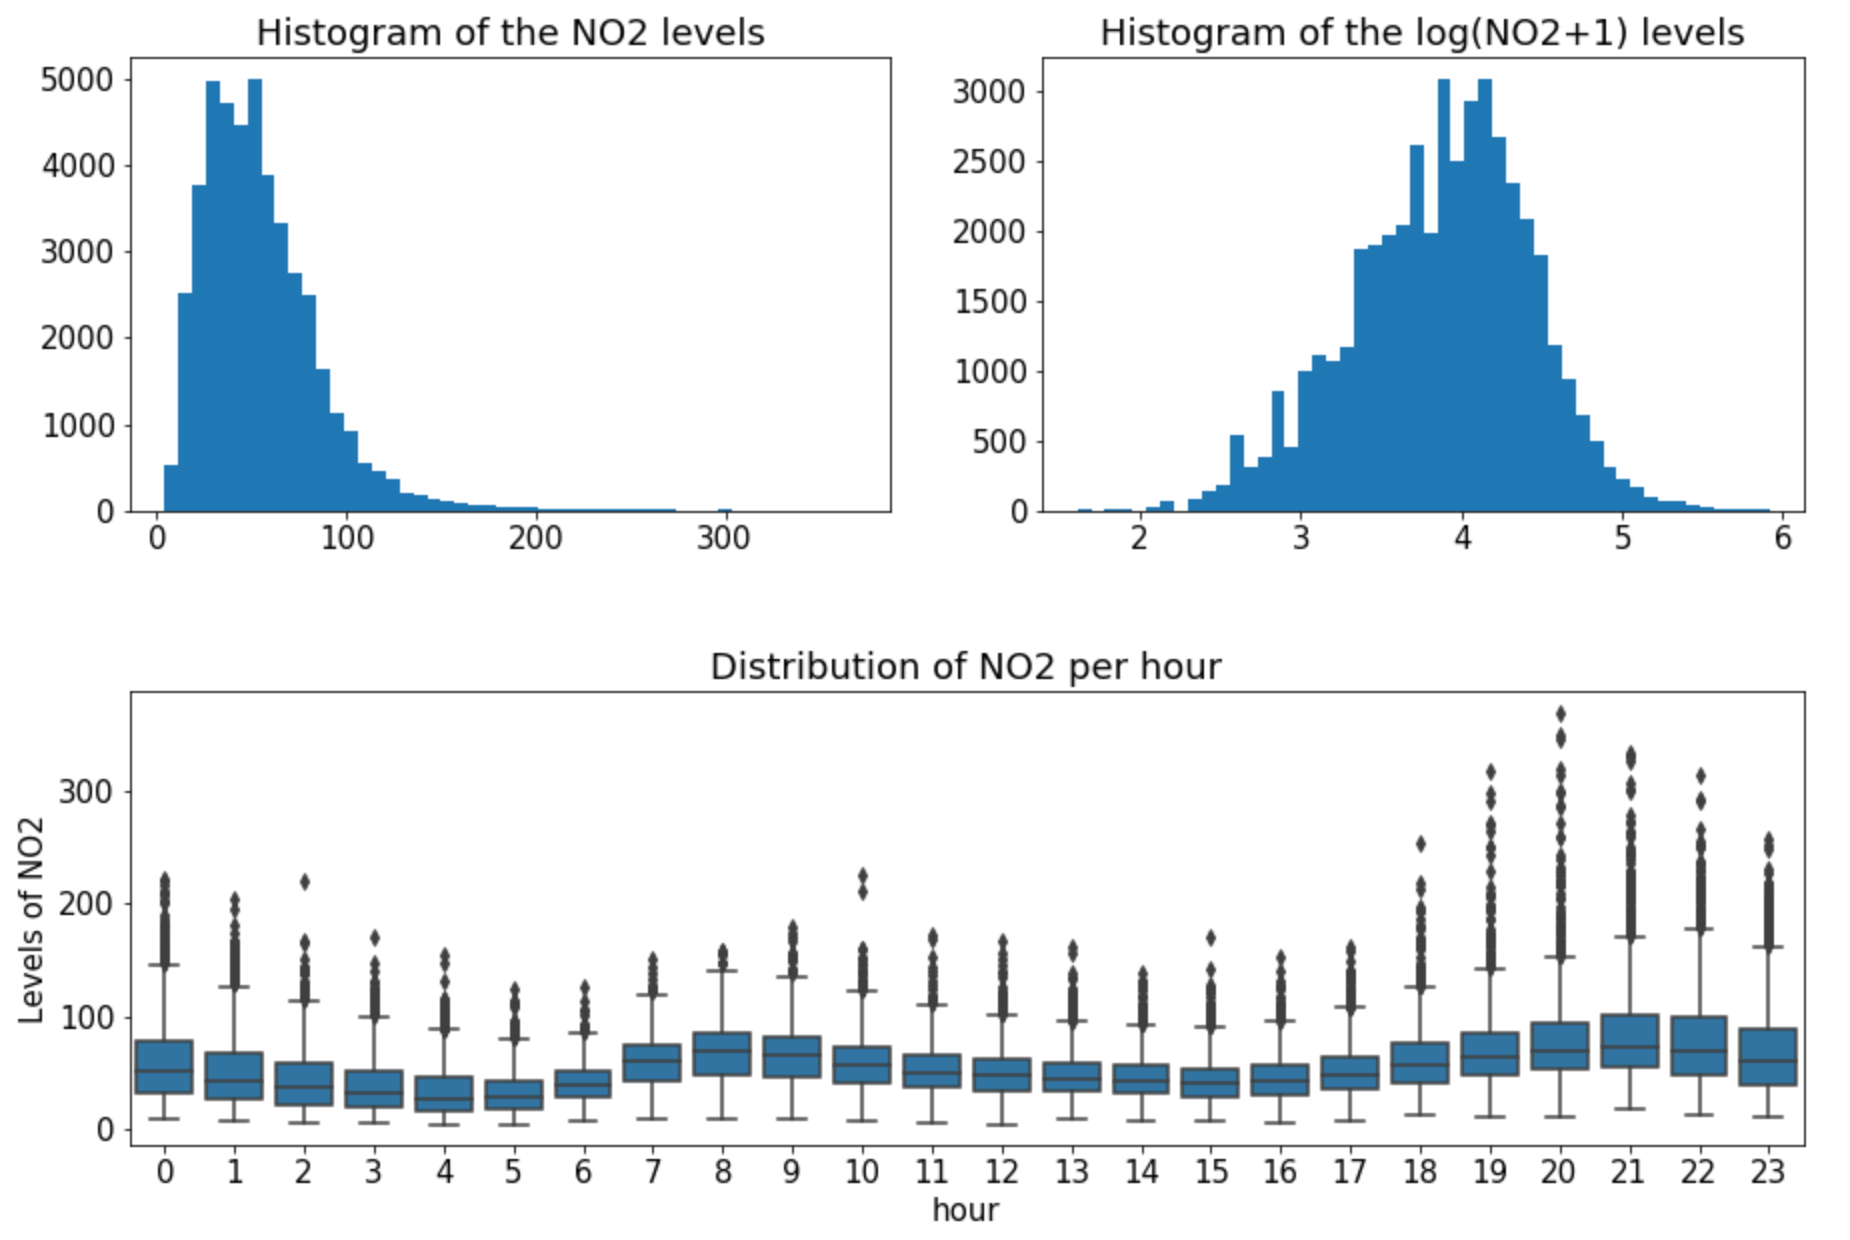
\includegraphics[width=0.8\textwidth]{histo_variance}
  \caption{\label{figure:histo_variance}Distribution of logarithmic
    \no{} and distribution of \no{}
    per hour.}
\end{figure}

\section{Data}
\label{data:sources}
\subsection{Air quality pollutants}
Hourly measurements of key air pollutants – Nitrogen dioxide (\no), Ozone (\ot), and Particulate Matter (\pmtwo, \pmten) – are gathered across Madrid via a network of 24 dedicated air quality stations (Figure \ref{figure:stationmap}). \no{}, a reddish-brown gas known for its pungent smell, has both natural and human origins, with fossil fuel combustion being the main source. Ground-level ozone (\ot) is generated in the atmosphere when pollutants (from traffic, industry, etc.) react chemically under the sunlight. \pmtwo{} and \pmten{} correspond to particles smaller than 2.5 and 10 micrometers in diameter respectively. These particles pose health risks as they can be inhaled deep into the lungs and potentially absorbed into the circulatory system. Combustion processes, including vehicle engines, power plants, and domestic burning, are primary sources.

\begin{figure}
  \centering
  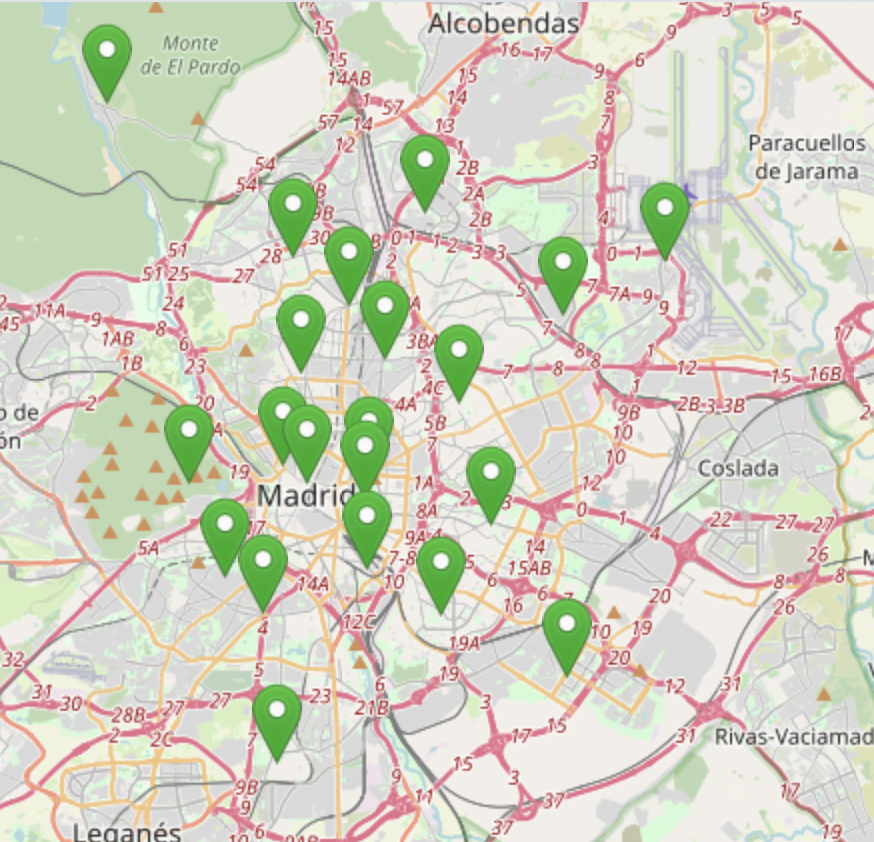
\includegraphics[width=0.6\textwidth]{stations}
  \caption{\label{figure:stationmap}Location of the 24 air quality monitoring stations.}
\end{figure}

\subsection{Numerical weather predictions}
Numerical weather predictions (NWP) are obtained from the Agencia Estatal de Meteorología (AEMET) \citep{meteorologia_agencia_nodate}, the Spanish state agency responsible for meteorology and forecasting. AEMET provides hourly measurements and forecast data for the following meteorological variables:
\begin{itemize}
    \item Boundary layer height (m): Height in the atmosphere where the earth's surface stops directly influencing the movement of air masses.
    \item Surface pressure (Pa): The pressure exerted by the atmosphere at ground level.
    \item Temperature (K): Ambient air temperature measured at a standard height of 2m.
    \item Precipitation (mm): The cumulative amount of water falling from the atmosphere to the surface (rain, snow, etc.)
    \item Wind speed (m/s): Horizontal wind velocity recorded at 10m above ground.
\end{itemize}
The native spatial resolution of the AEMET NWP is a 0.05° × 0.05° regular grid. Since data is required at the specific coordinates of the air quality stations, values were estimated using interpolation based on the nearest available grid nodes.

\subsection{Indicator predictions}
Air quality indicator forecasts are obtained from the Copernicus Atmospheric Monitoring Service (CAMS) \citep{cams}, managed by the ECMWF. CAMS generates hourly european pollution forecasts up to four days. It uses an ensemble technique that integrates outputs from seven distinct air quality models \citep{marecal_regional_2015}. Although the CAMS data, provided on a geodesic grid with 10-20 km spacing, lacks the fine resolution for pinpointing inner-city pollution patterns, it offers valuable insight into broader regional air quality trends. We incorporated the CAMS forecast concentrations for \ot, \no, \pmtwo{}, and \pmten{}. The value assigned to each air quality station was determined by selecting the prediction from the closest CAMS grid cell.

\subsection{Calendar Variables}
Since human activity is a primary driver of NO2 levels, we introduced variables to account for distinct daily patterns. Days were classified based on expected activity levels, identifying categories like bank holidays, school holidays, and significant traffic events (such as holiday travel returns). 

\subsection{Temporal Scope of Data}
The dataset consists of hourly measured concentrations whose timeframe ranges from 01/01/2013 through 31/12/2019. Data after 2019 was intentionally omitted from the analysis due to the profound impact of the COVID-19 pandemic, which significantly changed human activity patterns and therefore environmental conditions.

\section{Data pre-processing for Experiment 1}

This section details the data preparation strategy used for the first set of experiments, presenting key stages such as logarithmic transformation, the generation of additional variables via Fourier analysis and periodic functions, and the incorporation of lagged values. 

\subsection{Logarithmic Transformation}
We apply a logarithmic transformation to the values because the data's histogram shape seem to approximate a lognormal distribution. This approach offers two main benefits: first, it reduces the impact of the distribution's long tail as it reduces the range of values. Secondly, it reduces the data's skewness which is helpful for linear models such as the linear quantile regression.

\subsection{Engineering Periodic Features}
To analyze the target value's seasonality, we perform a Fourier transform and extract the 5 principal frequency components. These components correspond to the main season patterns found in the series and were clearly visible within the first 3000 elements of the transform output. The analysis revealed seasonality around 12h, 24h, 1 week (168h), and one year periods.
Based on these findings, we created periodic features using sine and cosine functions whose frequencies matched the identified cycles (12-h, 24-h, weekly, and annual). Including these variables as inputs helps the machine learning models learn the time series' seasonality.

\subsection{Lagged Values Features}
Following common practice in machine learning forecasting \citep{hyndman2021}, we incorporate lagged variables as inputs. The choice of lags is constrained by the prediction horizon and the need to limit the number of input features to avoid the curse of dimensionality \citep{bishop2006} and multicollinearity issues \cite{gujarati2009}. In our specific case, we capture lags from the immediate past (1–5 hours prior) and based on the seasonal analysis, we also included lags spaced approximately 11–13 hours apart, extending back up to 9 days. Additionally, we also add lags of 1, 2, and 7 days for the relevant calendar variables.

\section{Data pre-processing - Experiment 2 and 3}

\subsection{Data Preparation Framework}
\label{data:pre-processing} 
As previously stated, this research uses data collected from a network of 24 air quality stations scattered throughout Madrid. We obtain 24 distinct time series, each containing 4 specific indicators then we add four from the Copernicus Atmosphere Monitoring Service (CAMS), and five derived from Numerical Weather Prediction (NWP) models. From the lessons learned in the previous experiment and latest innovations, we improve the data pre-processing step with an updated sequence of operations involving data imputation, logarithmic transformation, deseasoning, and detrending. 

\subsection{Data Imputation}
Data from the multiple sources (Section~\ref{data:sources}) contains missing values, which must be addressed for reliable time series forecasting. Factors like sensor malfunctions or routine maintenance \citep{wardana_estimation_2022} are the origin of such gaps. Instead of developing new imputation methods, this study uses the procedures defined in a prior work by \citet{de_medrano_socaire_2021}. Briefly, the approach involved:
\begin{itemize}
    \item Single missing values: Filled using simple interpolation.
    \item Longer gaps (days/weeks): Addressed with source-specific techniques:
    \begin{itemize}
        \item[-] \textit{NWP data:} Imputed via trigonometric interpolation (Fourier series).
        \item[-] \textit{CAMS predictions:} Imputed using an X-ARIMA model with NWP data as an exogenous variable.
        \item[-] \textit{Air quality data:} Primarily imputed using X-ARIMA with CAMS and NWP data as exogenous variables. In some extreme cases, an HMISC method was additionally applied to the sensor data.
    \end{itemize}
\end{itemize}

\subsection{Data Transformation and Deseasoning}
Following the imputation phase, a logarithmic transformation was applied to all time series. This step helps reduces the variance and scales down the magnitude of the values. This also helps reducing exponential growth patterns into linear ones, further reducing the difficulty of predicting the patterns of the data. Aditionally, the 24-hour seasonality present in the time series is removed using a "Seasonal and Trend decomposition using Loess" (STL) method, as introduced by \citet{cleveland1990stl}. Removing this daily cyclical component simplifies the forecasting and allows the models to focus on other patterns without needing to explicitly predict this daily seasonality.

\subsection{Input Structuring via Rolling Windows and Detrending}
\label{dataprep:rollingwindow} 
As the deep learning models need sequential data as input, we are building rolling windows. Each input window consists of a sequence of the 168 most recent hourly values, which corresponds to the last previous 7 days relative to the forecast time point. The choice of a 7-day (168-hour) lookback period is based on the assumption that this timeframe captures the most relevant information for the prediction. 
As a final refinement step applied to each window individually, a detrending procedure is implemented. We evaluate the linear trend component within the window using the STL method and we subtract this trend value (specifically, the trend component estimated at the final hour of the window) from all data points within that window. This window-specific detrending aims to reduce the influence of short-term or local trends on the forecast and helps maintain the data values within a range less likely to cause saturation issues in the machine learning models. This data pre-processing step is inspired from the works of \citet{hewamalage_advancing_2022}.

\section{Metrics}

\label{experiment:metrics}
To comprehensively assess the performance of the proposed probabilistic forecasting models, we use a set of evaluation metrics. These metrics are chosen to evaluate different aspects of the forecast quality: the accuracy of the 50th quantile of the predicted distribution and the fit of the predicted distribution. We also analyze how well the models can forecast pollution peaks (values > 180$\mu g/m^3$)

\subsection{Mean Absolute Error (MAE)}
\label{sec:mae}
The Mean Absolute Error (MAE) quantifies the average of the errors between predicted values and observed outcomes. It is calculated as the mean of the absolute differences across all predicted points. In MAE, all errors are weighted equally in the average, making it less sensitive to large outliers compared to other metrics like RMSE. For our probabilistic models, the error is calculated with the median of the forecasted distribution. The MAE is computed as:

\begin{equation}
\label{eq:mae}
\text{MAE} = \frac{1}{N} \sum_{i=1}^{N} | \hat{y}_i - y_i |
\end{equation}

where \( \hat{y}_i \) is the predicted value, \( y_i \) is the corresponding observed value, and \( N \) is the total number of data points evaluated.

\subsection{BIAS}
The BIAS metric assesses if the model overestimate or underestimate the true values. It is computed as the average difference between the predicted values and the actual observations. Also note that a value close to zero does not guarantee high accuracy (as positive and negative errors can cancel out). The formula is:
\begin{equation}
\label{eq:bias}
\text{BIAS} = \frac{1}{N} \sum_{i=1}^{N} (\hat{y}_i - y_i)
\end{equation}
where \( \hat{y}_i \), \( y_i \), and \( N \) are defined as for the previously defined MAE.

\subsection{RMSE}
The Root Mean Square Error (RMSE) represents the standard deviation of the prediction errors (also called residuals). It is calculated as the square root of the average of the squared differences between predictions and actual observations. Due to the squaring operation, it penalizes larger errors more heavily than MAE. The formula is:
\begin{equation}
\label{eq:rmse}
\text{RMSE} = \sqrt{\frac{1}{N} \sum_{i=1}^{N} (\hat{y}_i - y_i)^2}
\end{equation}
where \( \hat{y}_i \), \( y_i \), and \( N \) are defined as previously. 

\subsection{CRPS}
Unlike metrics focused on point estimates like RMSE and MAE, the Continuous Ranked Probability Score (CRPS) \citep{hersbach_decomposition_2000} assesses both the calibration (reliability) and sharpness of a probabilistic forecast by comparing the forecast's cumulative distribution function (CDF), \( F \), against the empirical CDF of the observation \( y \) (a step function). It is calculated using the integral form:
\[
\text{CRPS}(F,y) = \int (F(x) - 1_{\{x \geq y\}})^2 \, dx
\]

\subsection{Normalized metrics}
We see that the pollutant levels vary widely across the air quality stations, reflecting the diverse environmental conditions within the same urban area. This makes it difficult to compare fairly the different metrics for different stations. However as described in Section \ref{data:pre-processing}, the input time series for each station undergo normalization and detrending procedures before being fed into the models. Therefore, the models produce forecasts in this transformed, normalized space. To enable a fair comparison of model performance across stations, we calculate the evaluation metrics (MAE, BIAS, RMSE, CRPS) using these normalized forecasts. These resulting 'normalized metrics' allow for a fairer assessment of model performance.

\subsection{Reliability and Sharpness Diagrams}
Beyond summary scores like CRPS, visual diagnostic tools are essential for understanding the performance of the probabilistic forecasts. We use Reliability and Sharpness Diagrams, as discussed in \cite{gneiting_probabilistic_2007}, for this objective. The reliability diagram checks if the forecasted probabilities actually match the actual observations. For this, it plots the actual probability of the observations vs the predicted probability of the observations. Therefore, a perfect forecast would have points lying on the diagonal line (y=x). If the points are below the diagonal, the model predicts higher probabilities than what really occurs. If points are above the diagonal, it predicts lower probabilities than what happens. The sharpness diagram is a histogram showing how often the actual observations' probability fell in a certain group (usually grouped in deciles). In probabilistic forecasts, this diagram should show that each group of probabilities have roughly the same number of observations. If the edge probabilities have more observations, it means that a higher number of observations fell in the tail of the predicted probability and therefore the uncertainty is underrepresented and the model overfits. On the contrary if the middle probability (around the median) has more observations, it means the undertainty is over-represented and the model underfits. By looking at both diagrams together, we get a good picture of the forecast quality: Reliability tells us if the probabilities are correct on average, and sharpness show the actual fit of those predictions.

\subsection{Peak Detection}
\label{peak_detect}
Understandably, the main application of these forecasts is predicting high pollution events, specifically when \no{} exceeds the 180$\mu g/m^3$ threshold, which is relevant for triggering emergency protocols. Standard classification metrics are inadequate due to the rarity of peak events, which can make accuracy misleading, and the asymmetric costs associated with prediction errors: indeed, emergency protocols often involve stopping human activity which has a high economic cost. Indeed false positive (FP), predicting a peak that does not occur, results in costly and disruptive interventions like traffic restrictions. While metrics like recall measure the fraction of actual peaks detected and precision assesses the reliability of peak predictions, neither fully captures this trade-off, particularly the disproportionately high cost of FPs. We then decide to directly compare model performance based on the resulting counts of True Positives (TP), representing correctly identified peaks, and False Positives (FP), representing false alarms. 

\section{Training/Test Data Split}
\label{exp:test}
When creating training and testing datasets for time series forecasting, the traditional approach is Out-of-Sample (OOS) evaluation. This involves splitting the time series chronologically, using an initial continuous partition for training the model and reserving the final partition for testing. This method respects the temporal order, avoiding the use of future data to predict the past. However, this single test set can be highly variable and not be representative of future outcomes, especially with limited data.

On the other hand, standard K-fold cross-validation (CV), while common in regression and classification, is often avoided for time series due to concerns about training the model with data that is posterior to the test element (as K-fold shuffles the data). However, \citet{bergmeir_note_2018} argues for the validity of standard K-fold CV for purely autoregressive time series models, provided the model errors are uncorrelated. This condition is often met when using models that can capture the underlying dynamics well resulting in uncorrelated residuals. This procedure requires first creating a standard K-fold CV with the data and split it into K folds. Then, when a fold is assigned to a test fold, the rows in the training set that have a time step in the test set are dropped. They show this approach can provide more precise error estimates than OOS. The main drawback from this procedure is that it requires a lot of compute power, specially if the models are long to train like deep learning models.

Therefore, due to our limits on compute power, we use a K-fold cross-validation for machine learning models and an Out-of-Sample evaluation for deep learning models.

\section{Hyperparameter search}
Hyperparameters are machine learning model parameters which controls diverse settings of those models like model complexity, regularization or optimization algorithm (e.g., learning rate, number of layers, tree depth). Selecting the appropriate hyperparameters is necessary for achieving the optimal model performance. This process is known as hyperparameter tuning. We describe below the 2 hyperparameter strategies we use in this research:

The first method we could apply is to simply test all possible combinations and select the best hyperparameter combination. This exhaustive method, called Grid Search, defines a discrete grid of hyperparameter values and evaluates the model performance for every combination of hyperparameters. While simple to implement and guaranteed to find the best combination within the specified grid, its computational cost grows exponentially with the number of hyperparameters and the density of the grid. Therefore, it is not practical for highly intensive models like deep learning models or even for simpler models when the high-dimensional search space requires too many combinations to evaluate.

To improve from grid search, random search \citep{Bergstra2012} could be used. This method consists on sampling hyperparameter configurations randomly from the search space. It is indeed more efficient, as it is more likely to find truly influential hyperparameters within a fixed budget. However, its effectiveness can be limited if the number of random samples is small relative to the vastness of the search space. Bayesian Optimization \citep{humanout} offers a more directed approach. By building a probabilistic model of the objective function (in our case the validation error) and intelligently selecting the next hyperparameters to evaluate. Given the advantages of this guided search strategy, we employ the Sequential Model-based Algorithm Configuration (SMAC) framework \citep{JMLR:v23:21-0888}, a robust implementation of Bayesian optimization, for our hyperparameter tuning. This method searches through a Gaussian process the hyperparameter values that minimize the cost function of the model (in our case the negative log likelihood). 

\section{Post-hoc Calibration Methods} 
\label{exp:posthoc}
While shallow neural networks are well calibrated as shown by \citep{niculescu-mizil_predicting_2005}, deep neural networks, albeit superior in accuracy, are not so well calibrated \citep{guo_calibration_2017}. This discrepancy between accuracy and calibration means that the probability estimates produced by these advanced models do not represent the true uncertainty.

As stated by \citep{wang_calibration_2024}, several post-hoc methods have been developed to address this issue. Many of these methods are applied for classification tasks and are not suitable for out probabilistic regression application, where the full probability distribution of the target is predicted. However, we can adapt some of those methods for this case. Those methods can be classified into parametric and non-parametric methods.

Parametric transformations are based on a mapping function with a fixed number of parameters using a dedicated calibration dataset. In classification tasks, Temperature Scaling \citep{guo_calibration_2017}, which is a variation of Platt Scaling \citep{Platt1999}, adjusts the logits output of a neural network by a single scalar parameter (the "temperature") before the softmax function, thereby "softening" or "sharpening" the output probabilities to better align with empirical correctness. \citet{kuleshov18a} adapted the concept for probabilitic regression tasks and introduced the idea of applying a learned temperature-like scalar to directly modify the predicted variance of the output distribution. If the model predicts the parameters of an output distribution (e.g., mean $\mu$ and standard deviation $\sigma$ for a Gaussian), we can use the temperature to adjust the variance of the output distribution. This indeed addresses the calibration of the uncertainty estimate by scaling the predicted spread. This temperature is estimated by minimizing the negative log likelihood metric in the calibration set.

On the other hand, non-parametric transformations are more flexible as they do not assume a specific functional form for the calibration map. The first example of those methods is histogram binning \citep{Zadrozny2001HB}. This method groups predictions from the original model into a set of bins based on their initial confidence or predicted values. A new calibrated probability is then assigned to all predictions falling within a particular bin, typically derived from the empirical outcomes of calibration samples in that bin. For regression, this could involve binning by the predicted mean $\mu$ and then re-estimating both $\mu$ and $\sigma$ for each bin based on the true values and prediction errors within it. 
Another technique, quantile mapping (QM) was introduced in the context of bias correction for climate model outputs by \citet{patel_quantile_2022}. QM aligns the cumulative distribution function (CDF) of the model's predictions with the CDF of the observed true values from a calibration period. For a new prediction, its value is transformed by first finding its quantile in the model's predicted distribution and then mapping this quantile to the corresponding value in the observed distribution. This method corrects the entire distribution of predictions. 

Also hybrid approaches have also been proposed. For instance, scaling binning \citep{kumar_verified_2020} combines the strengths of parametric and non-parametric methods. It first applies a parametric scaling function (like temperature scaling) to the initial model outputs to reduce variance and improve general calibration. Subsequently, the outputs of this scaling function are binned, and the final calibrated output for a new prediction is determined by the average of the scaled values within the bin it falls into. This two-step process aims to achieve both the sample efficiency of scaling methods and the measurable calibration error guarantees associated with binning.

\section{Experiments}

\subsection{Experiment 1: Comparing classical machine learning probabilistic models}

The primary objective of this experiment is to compare the performance of the classical machine learning models introduced in Section 3.1 for probabilistic air quality forecasting. Specifically, we focus on forecasting the probability distribution of hourly Nitrogen Dioxide (\no{}) concentrations, as they are the sole indicator whose peak levels trigger the emergency protocol. This evaluation is conducted for a single and representative monitoring station, Escuelas Aguirre in Madrid, across a range of future horizons from 1 hour up to 60 hours ahead.

The input dataset for this experiment comprises hourly air quality measurements (\no{}, \ot{}, \pmtwo{}, \pmten{}) from the different air quality stations alongside CAMS data and engineered calendar variables as detailed in Section 4.3. Before training, we apply a pre-processing pipeline to the data, as described in Section 4.4, which includes applying a logarithmic transformation to the target variable (\no{}), generating periodic features based on Fourier analysis to capture seasonality, and incorporating lagged values of relevant predictors.

As the models require relatively low compute power, we can use a K-fold cross-validation test (Section 4.6) on the historical data spanning from January 1, 2013, to December 31, 2019 (Section \ref{exp:test}). We use an Exhaustive Search (Grid Search) to select the hyperparameters of the models. Once the models are trained, we use them to generate probabilistic forecasts for each hour in the test set, covering all 60 future horizons. The quality of these forecasts is evaluated through an exhaustive list of metrics as defined in Section 4.5, including MAE, BIAS, RMSE, CRPS and reliability/sharpness diagrams. These metrics are calculated independently for each forecast horizon.

\subsection{Experiment 2: Comparing deep learning probabilistic models}

This experiment aims to evaluate and compare the performance of the deep learning based models introduced in Section 3.2 (LSTM, CNN, and Transformer based architectures) for probabilistic air quality forecasting. We would benchmark them against the best model from the previous classical machine learning models experiment: QGB (Section \ref{model:qgb}), which we name in this experiment QGBT to indicate that it's using the updated data pre-processing. The objective is to predict the probability distribution of hourly Nitrogen Dioxide (\no{}) levels across all monitoring stations in Madrid, focusing only on the 13-hour forecast horizon. We are also applying Global Forecasting Models (GFMs), where the models are trained with multiple time series instead of just a single one. Indeed, several time series from different sources are available as input and they can contribute to training the models in different ways. On one hand, we could build a univariate global model trained with several time series that could forecast all the \no{} time series. The univariate models are the simplest models and as suggested by \citet{hewamalage_recurrent_2021} should incorporate cross-information from the time series when used as Global Forecasting Models. On the other hand, we build a multivariate forecasting models with a multivariate time series as input (with all the data available in a station as input). On top of investigating the impact of varying the input dimensionality (univariate vs. multivariate inputs), we also evaluate how increasing the volume of training data impacts performance (input data ranges from \no{} levels on a single station, all \no{} time series available, similar time series and finally all the available time series). 

Given the distinct computational demands and tuning challenges associated with deep learning architectures, we decide to conduct this experiment in two main phases. First, we focus on the LSTM and CNN models and then on the transformer models. In both phases, the input data for these models undergoes the pre-processing pipeline described in Section 4.5. This includes data imputation, logarithmic transformation, deseasoning using STL, and structuring the data into sequential rolling windows of 168 hours with window-specific detrending. This results in a sequence-based input for the deep learning architectures. 

As described in Section 4.7 regarding computational constraints for deep learning models, we test with an an Out-of-Sample (OOS) evaluation strategy. Data from January 1, 2013, to December 31, 2018, represents the training set, while we test with data from January 1, 2019, to December 31, 2019. 

Taking into account all possible combinations of model architectures, input dimensionality (univariate/multivariate), training data scopes, and MLP output configurations (1 vs. 2), we arrive at 30 distinct experimental setups in phase 1 and 12 in phase 2. To facilitate clear referencing and discussion, each experimental configuration is assigned a concise identifier, as listed in Table \ref{tab:exp2_combin} and schematically represented in Figure \ref{fig:exp2_nom}.

\begin{figure}[h] 
  \centering  
  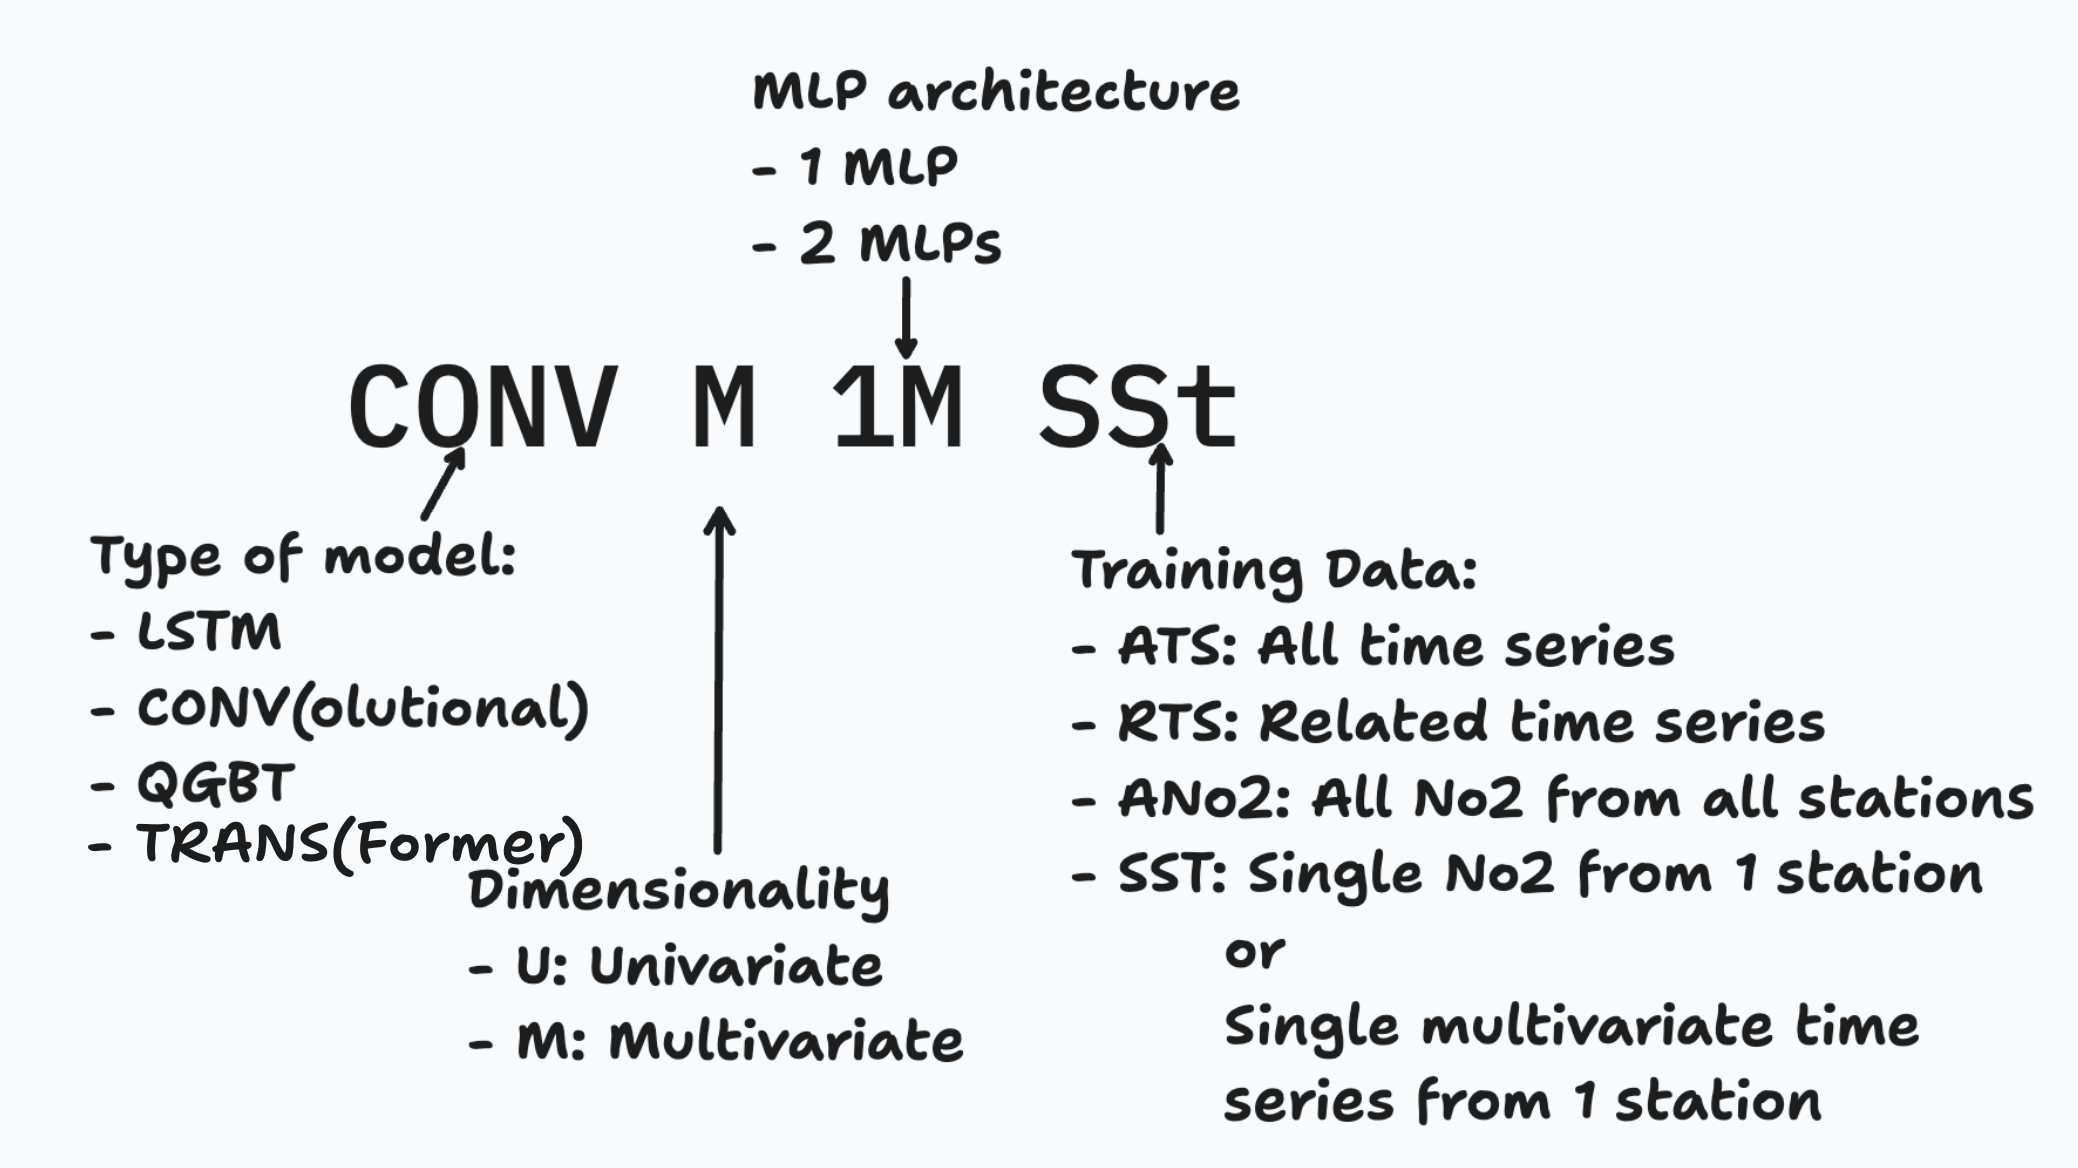
\includegraphics[width=.7\textwidth]{nom.png}
  \caption{Explanation of short nomenclature of experimental configurations }
  \label{fig:exp2_nom}
\end{figure}

\begin{table}[h]
\centering
\begin{tabular}{lllll}
\toprule
Model Family & Model Dimension & MLPs &             Input Data &      Short name \\
\midrule
        LSTM &      Univariate &    1 &     \no from 1 station &   LSTM U 1M SST \\
             &                 &    1 &  \no from all stations &  LSTM U 1M A\no \\
             &                 &    1 &    Related time series &   LSTM U 1M RTS \\
             &                 &    1 &        All time series &   LSTM U 1M ATS \\
             &    Multivariate &    1 &              1 station &   LSTM M 1M SST \\
             &                 &    1 &           all stations &   LSTM M 1M ATS \\
        LSTM &      Univariate &    2 &     \no from 1 station &   LSTM U 2M SST \\
             &                 &    2 &  \no from all stations &  LSTM U 2M A\no \\
             &                 &    2 &    Related time series &   LSTM U 2M RTS \\
             &                 &    2 &        All time series &   LSTM U 2M ATS \\
             &    Multivariate &    2 &              1 station &   LSTM M 2M SST \\
             &                 &    2 &           all stations &   LSTM M 2M ATS \\
        CONV &      Univariate &    1 &     \no from 1 station &   CONV U 1M SST \\
             &                 &    1 &  \no from all stations &  CONV U 1M A\no \\
             &                 &    1 &    Related time series &   CONV U 1M RTS \\
             &                 &    1 &        All time series &   CONV U 1M ATS \\
             &    Multivariate &    1 &              1 station &   CONV M 1M SST \\
             &                 &    1 &           all stations &   CONV M 1M ATS \\
        CONV &      Univariate &    2 &     \no from 1 station &   CONV U 2M SST \\
             &                 &    2 &  \no from all stations &  CONV U 2M A\no \\
             &                 &    2 &    Related time series &   CONV U 2M RTS \\
             &                 &    2 &        All time series &   CONV U 2M ATS \\
             &    Multivariate &    2 &              1 station &   CONV M 2M SST \\
             &                 &    2 &           all stations &   CONV M 2M ATS \\
        TRANS &      Univariate &    1 &     \no from 1 station &   TRANS U 1M SST \\
             &                 &    1 &  \no from all stations &  TRANS U 1M A\no \\
             &                 &    1 &    Related time series &   TRANS U 1M RTS \\
             &                 &    1 &        All time series &   TRANS U 1M ATS \\
             &    Multivariate &    1 &              1 station &   TRANS M 1M SST \\
             &                 &    1 &           all stations &   TRANS M 1M ATS \\
        TRANS &      Univariate &    2 &     \no from 1 station &   TRANS U 2M SST \\
             &                 &    2 &  \no from all stations &  TRANS U 2M A\no \\
             &                 &    2 &    Related time series &   TRANS U 2M RTS \\
             &                 &    2 &        All time series &   TRANS U 2M ATS \\
             &    Multivariate &    2 &              1 station &   TRANS M 2M SST \\
             &                 &    2 &           all stations &   TRANS M 2M ATS \\
        QGBT  &      Univariate &    X &     \no from 1 station &      QGBT U SST \\
             &                 &    X &  \no from all stations &     QGBT U A\no \\
             &                 &    X &    Related time series &      QGBT U RTS \\
             &                 &    X &        All time series &      QGBT U ATS \\
             &    Multivariate &    X &              1 station &      QGBT M SST \\
             &                 &    X &           all stations &      QGBT M ATS \\
\bottomrule
\end{tabular}
\caption{All experimental configurations in the experimental design}
\label{tab:exp2_combin}
\end{table}

The hyperparameter optimization is performed using the Sequential Model-based Algorithm Configuration (SMAC) framework detailed in Section 4.8. For each model configuration (architecture type, input type, training data scope), SMAC performs 150 trials to find the optimal set of hyperparameters based on minimizing the negative log-likelihood of the validation set. We still find this process to be very time consuming due to the heavy load of the deep learning models. Therefore we limit the training time on each trial to reduce significantly the execution time (it is reduced to 3 days instead of 16 days). However, the hyperparameter search for the QGBT models takes much longer to execute as their architecture does not allow to limit the training time. Additionally, this time limit is only performed for the hyperparameter search, and once these are found, the final model training does not have any time restriction.  However for the second phase, preliminary attempts to use the same SMAC strategy as in phase 1 for Transformers proved problematic. The Transformer models have a significantly larger hyperparameter space and are much more computationally intensive per epoch. Furthermore, SMAC struggled with frequent errors caused by hyperparameter combinations leading to models too large for GPU memory and SMAC often interpreted these failures as simply poor performance, hindering effective exploration. Consequently, a modified, more constrained hyperparameter search was adopted for Transformers. The search space for hyperparameters was significantly reduced and only 10 SMAC trials were conducted per configuration. Instead of limiting the time execution per trial, the training was limited to 1 epoch. 

On both phases, once trained with the optimal hyperparameters, each model is used to predict the \no{} distribution on the test set (year 2019) on the 13th horizon. The models predict the parameters (mean and variance) of a Gaussian distribution. The performance of the models is evaluated using the metrics defined in Section 4.6, including normalized MAE, BIAS, RMSE, and CRPS, along with reliability and sharpness diagrams, and peak detection analysis (TP/FP counts for the threshold 180 $\mu g/m^3$). We then calculate the metrics across all model configurations and across all stations. 

\subsection{Experiment 3: Applying post-hoc calibration to deep learning probabilistic models}

The objective of this experiment is to investigate whether post-hoc calibration techniques can improve the probabilistic forecasts of the best-performing deep learning models identified in the previous experiment. This experiment aims to improve the calibration of the deep learning models by applying both individual and combined post-hoc adjustments specified in section \ref{exp:posthoc} and assess its impact on overall forecast quality, particularly on the same metrics and in the same test set as the previous experiment.

Then from the previous experiment, we select the top-performing configuration for each of the three deep learning architectures: Long Short-Term Memory (LSTM), Convolutional Neural Network (CNN), and Transformer. The data pre-processing steps (imputation, logarithmic transformation, deseasoning, rolling windows, and detrending as detailed in Section 4.5) for the input to the pre-trained models remain identical to those in Experiment 2. For each of these selected pre-trained models, we apply several post-hoc calibration methods: Temperature Scaling (TS), Quantile Mapping (QM), Scaling Binning (SB), and a simple Mean Bias Correction (BC), where the mean bias observed on the validation set is subtracted from the forecasts. Finally, to check for a combination of effects, we also evaluate a method that applies Quantile Mapping followed by Scaling Binning (QM+).

A dedicated calibration dataset is used. This calibration set is extracted from 5\% of the training dataset randomly sampled. The models not be trained with that data. Once the calibration procedures are applied, the calibrated models are re-evaluated on the same test set used in Experiment 2 (data from January 1, 2019, to December 31, 2019) for the 13-hour forecast horizon across all monitoring stations. The performance is assessed using the same metrics outlined in Section 4.6: normalized and standard MAE, BIAS, RMSE, and CRPS, alongside Peak Detection (TP/FP counts for the NO$_2$ threshold. 

The results from this experiment is compared against the uncalibrated performance of the same models from Experiment 2. This allows us to quantify the improvements, if any, brought by each post-hoc calibration technique.

\chapter{Results}

\subsection{Classical Machine Learning Experiment}

The performance of the different classical machine learning models is evaluated across forecast horizons ranging from 1 to 60 hours. Figure \ref{figure:exp1_metrics} provides a visual comparison of key performance metrics (MAE, BIAS, RMSE, CRPS) for each model.

\begin{figure}[tbp]
  \centering
  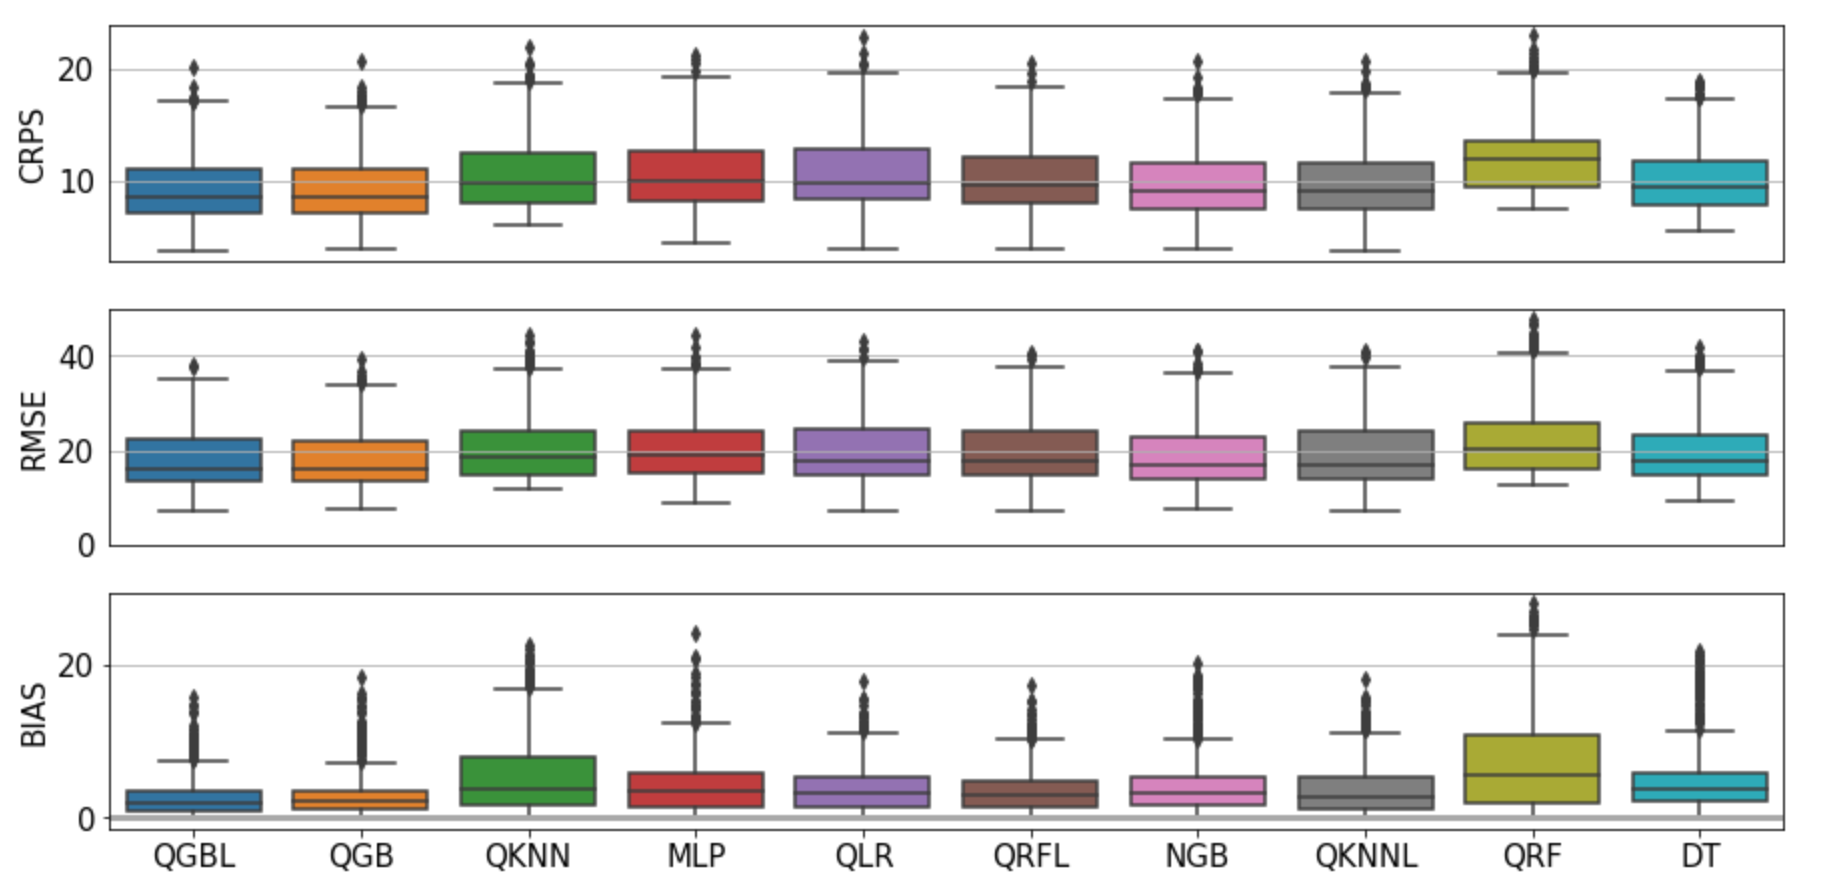
\includegraphics[width=0.95\textwidth]{exp1_metrics_chart.png}
  \caption{\label{figure:exp1_metrics}
    Boxplot of continuous ranked probability score, root mean squared
    error and bias of the different models for all horizons.
  }
\end{figure}

First, the linear dependency within the predictor variables explains why the simpler Quantile Linear Regression (QLR) achieves reasonable performance. However, QLR's inability to capture non-linear relationships limits its overall performance compared to more sophisticated approaches. In contrast, Quantile Random Forests (QRF) and Quantile k-Nearest Neighbors (QKNN) provide less accurate results and exhibit higher bias. 

Quantile k-Nearest Neighbors and Quantile Random Forest applied to residuals (QKNNL and QRFL) show surprisingly good performance. Notably, QKNNL achieves performance comparable to the top-performing QGB while requiring significantly less computational time for training, making it an attractive option considering its simplicity. 

However, across all metrics and horizons, the Quantile Gradient Boosted Trees (QGB) model consistently demonstrates superior performance compared to the other methods. The additive nature of gradient boosting enables modeling the complex and non-linear relationships present in the data. On the other hand, using QGB with the residuals (QGBL) does not provide substantial improvements over the standard QGB model. We believe QGB already learns the linear components effectively.

Finally, distributional Forests (DT) and Natural Gradient Boosted Trees (NGBoost) do not surpass the performance benchmark set by QGB. The use of natural gradients in NGBoost does not seem to offer an advantage for this particular forecasting task. Although the Multilayer Perceptron (MLP) model achieves good bias scores, it generally lags behind the gradient boosting methods in overall predictive accuracy.

Table \ref{tab:exp1_determ} shows the mean and standard deviation of the main metrics and the training times for each model. This further confirm the robust performance of QGB and also highlights the advantage of QKNNL that offers strong performance with remarkably low training times.

\begin{table}[tbp]
  \centering \footnotesize
  \caption{\label{tab:exp1_determ}Error measures for the proposed models.}
    \begin{tabular}{lrrlllll}
      \toprule
         method &              CRPS &              RMSE &             bias &                training time (s) \\
        \midrule
            NGB &  $ \underset{(3.3)}{10.0} $ &  $ \underset{(7.2)}{19.4} $ &  $ \underset{(4.3)} {4.6}$ & $ \underset{(83.4)}  {997.6}$    \\
          QKNNL &  $ \underset{(3.4)}{10.0} $ &  $ \underset{(9.7)}{20.1} $ &  $ \underset{(3.7)} {3.9}$ & $ \underset{(0.6)}     {8.3}$    \\
             DT &  $ \underset{(3.1)}{10.3} $ &  $ \underset{(7.3)}{20.0} $ &  $ \underset{(5.1)} {5.3}$ & $ \underset{(17.6)}  {732.9}$   \\
           QRFL &  $ \underset{(3.3)}{10.4} $ &  $ \underset{(9.5)}{20.6} $ &  $ \underset{(3.3)} {3.8}$ & $ \underset{(0.7)}    {10.5}$    \\
           QKNN &  $ \underset{(3.4)}{10.7} $ &  $ \underset{(7.8)}{20.9} $ &  $ \underset{(5.2)} {5.4}$ & $ \underset{(0.6)}     {8.2}$   \\
            MLP &  $ \underset{(3.3)}{10.8} $ &  $ \underset{(6.9)}{20.6} $ &  $ \underset{(4.1)} {4.5}$ & $ \underset{(43.3)}  {232.9}$   \\
            QLR &  $ \underset{(3.6)}{10.9} $ &  $ \underset{(8.9)}{20.7} $ &  $ \underset{(3.4)} {4.0}$ & $ \underset{(0.8)}     {9.7}$    \\
            QRF &  $ \underset{(3.4)}{12.2} $ &  $ \underset{(8.6)}{22.8} $ &  $ \underset{(6.9)} {7.5}$ & $ \underset{(1.7)}    {30.8}$    \\
            QGB &  $ \underset{(3.1)}{9.5}  $ &  $ \underset{(6.6)}{18.2} $ &  $ \underset{(3.4)} {3.3}$ & $ \underset{(8.5)}    {37.0}$    \\
           QGBL &  $ \underset{(3.2)}{9.5}  $ &  $ \underset{(9.9)}{19.0} $ &  $ \underset{(3.0)} {2.9}$ & $ \underset{(7.4)}    {36.0}$   \\
       \bottomrule
      \end{tabular}
\end{table}

While CRPS provides a valuable summary, reliability and sharpness diagrams (Figure \ref{figure:exp1_rel_sharp}) offer visual diagnostic insights into the quality of the probabilistic forecasts. NGBoost, MLP, and QKNNL display the most desirable flat histograms, suggesting their predicted uncertainty levels are well-calibrated. On the other hand, QRF, QRFL, QKNN, and DT exhibit histograms skewed towards the center, indicating their predictive distributions are often too wide which is a sign of underfitting. QGB, QGBL, and QLR show the opposite tendency, with higher frequencies in the tails, suggesting their distributions were often too narrow. This underestimation of the uncertainty is a sign of overfit, as the prediction is adjusting too much to the training data and not accounting the whole uncertainty.

\begin{figure}
  \centering
  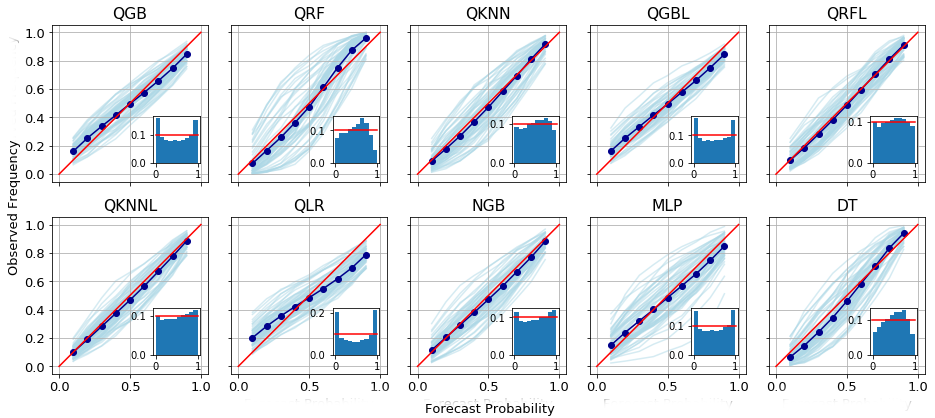
\includegraphics[width=0.99\textwidth]{exp1_relsharp.png}
  \caption{\label{figure:exp1_rel_sharp}Average reliability and sharpness
    of the different models across all horizons. The dim blue lines
    correspond to the different horizons. }
\end{figure}  

QGBL and QKNNL show the best calibration, with average reliability curves close to the ideal diagonal line and minimal variation across different forecast horizons. MLP and NGBoost also show good average calibration but show greater variability between horizons. QRF, QRFL, QKNN, and DT display higher variability reflecting their uncertainty estimation issues. QGB and QLR's results are in line with the overly narrow distributions. Finally, NGBoost and QKNNL appear particularly effective at predicting the upper tail of the distribution (e.g., the 90th quantile), which is relevant when forecasting pollution peaks.

\begin{table}[tbp]
  \centering \footnotesize
  \caption{\label{tab:exp1_quade}Average Rankings of the algorithms (Quade)}
  \begin{tabular}{c|c}
    Algorithm&Ranking\\
    \hline
    DT&4.864155251141552\\
    MLP&4.289954337899544\\
    NGB&6.81544901065449\\
    QGB&9.407153609071533\\
    QGBL&8.90677321156773\\
    QKNN&3.10806697108067\\
    QKNNL&6.51255707762557\\
    QLR&4.276255707762556\\
    QRF&1.4448249619482494\\
    QRFL&5.3748097412480975\\
    \end{tabular}
\end{table}

To assess the statistical validity of these comparisons, advanced non-parametric statistical tests are conducted \citep[as described by][]{garcia_advanced_2010}. The Quade test, applied across the 60 horizons, show a highly significant result (p < 0.001), confirming statistically meaningful differences in performance among the models. We can use this test to obtain a reliable ranking based on overall performance, presented in Table \ref{tab:exp1_quade}. This ranking corroborates the findings discussed above, with QGB and QKNNL on the top spots.

\subsection{Deep Learning Experiments}

The results of the deep learning experiments, designed to assess the capabilities of LSTM, CNN, and Transformer architectures for probabilistic air quality forecasting, are presented in this section. The presentation of these findings is structured into two subsequent phases. First, we delve into a comparative analysis focusing on the LSTM and CNN models relative to the QGBT benchmark. Following this, a separate comparison specifically addresses the performance of the Transformer-based models, again evaluated against QGBT.

\subsubsection{Focus on the LSTM and CNN Models}

\begin{figure}[h!]
  \centering
  % Use a wider width since the image contains two plots
  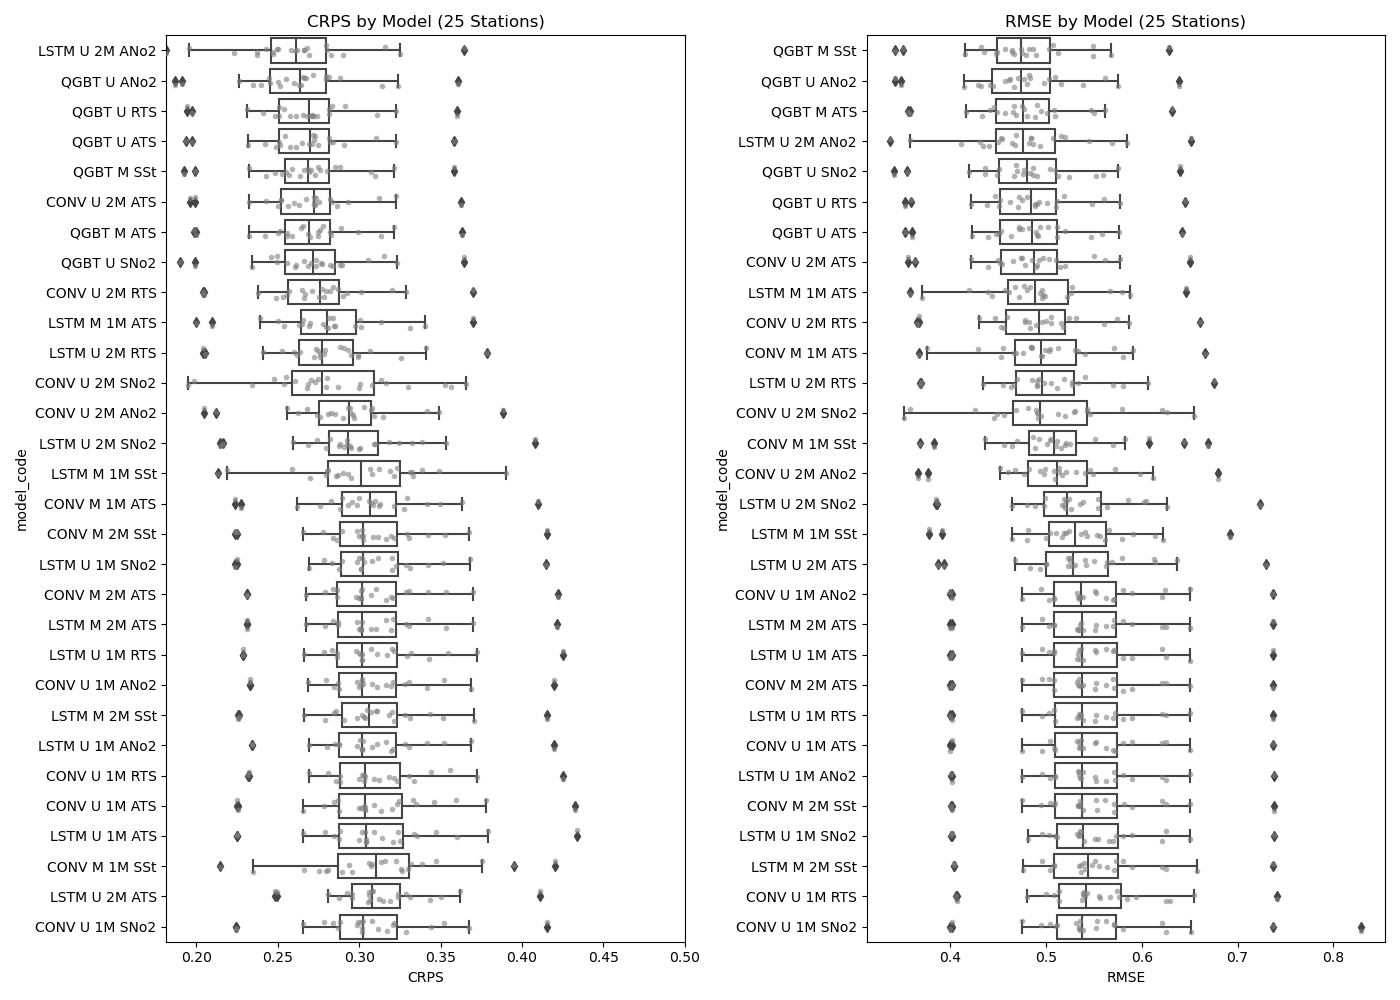
\includegraphics[width=\textwidth]{exp2a_rmse_crps.png} 
  \caption{Distribution of normalized CRPS (left) and RMSE (right) scores for each experimental configuration across all 25 stations. Models are sorted independently in each panel by their mean performance.}
  \label{fig:exp2a_rmse_crps_boxplot}
\end{figure}

This section details the performance evaluation of the LSTM and CNN experimental configurations outlined in Table \ref{tab:exp2a_complex1}. We use the metrics defined in Section \ref{experiment:metrics} to assess the impact of the architecture, input dimensionality (univariate vs. multivariate) and the scope of training data (single station, all \no{} series, related series, all series) for the 13-hour forecast horizon across all Madrid monitoring stations.

The performance of each configuration is detailed in Figure~\ref{fig:exp2a_rmse_crps_boxplot}, which presents the distribution of normalized CRPS and RMSE scores across all 25 stations. This figure consists of two panels, one for each metric, where the configurations are independently sorted by their mean performance. This visualization reveals a group of configurations achieving the best results: notably, all with the QGBT architecture and alongside, the Univariate LSTM model employing 2 Multi-Layer Perceptrons trained on all \no{} time series (LSTM U 2M ANO2), and the Univariate CONV model with 2 MLPs trained on all time series (CNN U 2M ATS). This ranking of these leading configurations is relatively consistent across stations.

To move beyond visual inspection and confirm the statistical significance of these observations, we employ non-parametric statistical tests. An initial Quade test \citep{garcia_advanced_2010}, comparing all 30 experimental configurations across the 24 stations based on mean CRPS values, had a low p-value ($\approx 1.11 x  10^{-16}$). The null hypothesis of this test states there's no difference in performance between the different configurations, which was rejected. The ranking of the Quade test can be seen in Figure \ref{fig:exp2a_pairwise}. However, we perform a robustness check on this test by repeatedly sampling CRPS values at random time points across all stations and running the Quade test on these samples. The resulting distribution of p-values robustly reinforces the significant difference between the configurations.

\begin{figure}[h] 
  \centering  
  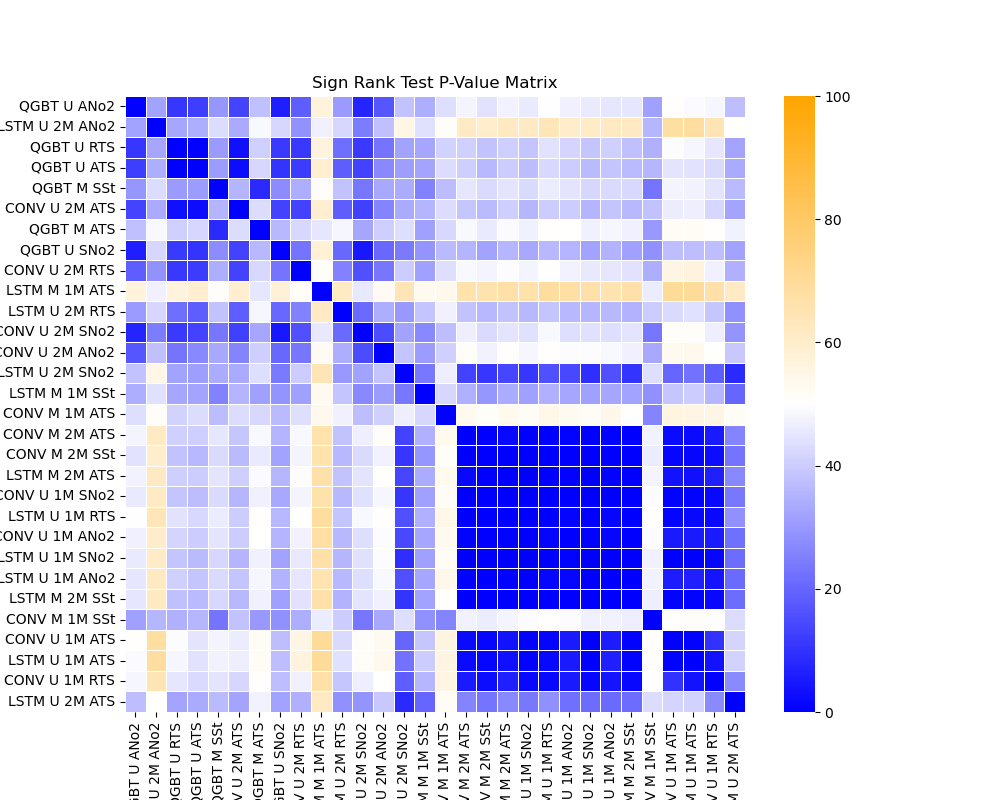
\includegraphics[width=1\textwidth]{exp2a_pairwise.png}
  \caption{Matrix of pairwise comparison between models}
  \label{fig:exp2a_pairwise}
\end{figure}

For a more detailed understanding of relative performance, pairwise comparisons between all experimental configurations are conducted using the Kolmogorov-Smirnov (KS) test. For each pair, we generate 1000 samples by randomly selecting a time point and collecting the CRPS scores from all 24 stations for both configurations. The KS test is applied to each sample pair to determine if their CRPS distributions were significantly different. We calculate the proportion of these 1000 tests where the null hypothesis is rejected at a significance level of $\alpha = 0.1$. We choose this value as a lower p-value was too strict to show differences between the models. Figure \ref{fig:exp2a_pairwise} presents a matrix visualizing these comparisons, ordered according to the ranking derived from the initial Quade test. This pairwise comparison matrix highlights distinct groups of models with statistically similar performance characteristics. The top-performing group includes the QGBT configurations and the previously mentioned deep learning contenders (LSTM U 2M ANO2, CNN U 2M ATS). Additionally, the lower performing group is populated by the deep learning multivariate configurations, suggesting that increasing input dimensionality not only does not translate into improved predictive performance but potentially hinders performance. Since the BIAS metric reveals minimal differences among the top‐performing models, it is not useful for selecting the best model in this experiment.

\begin{figure}[h] 
  \centering  
  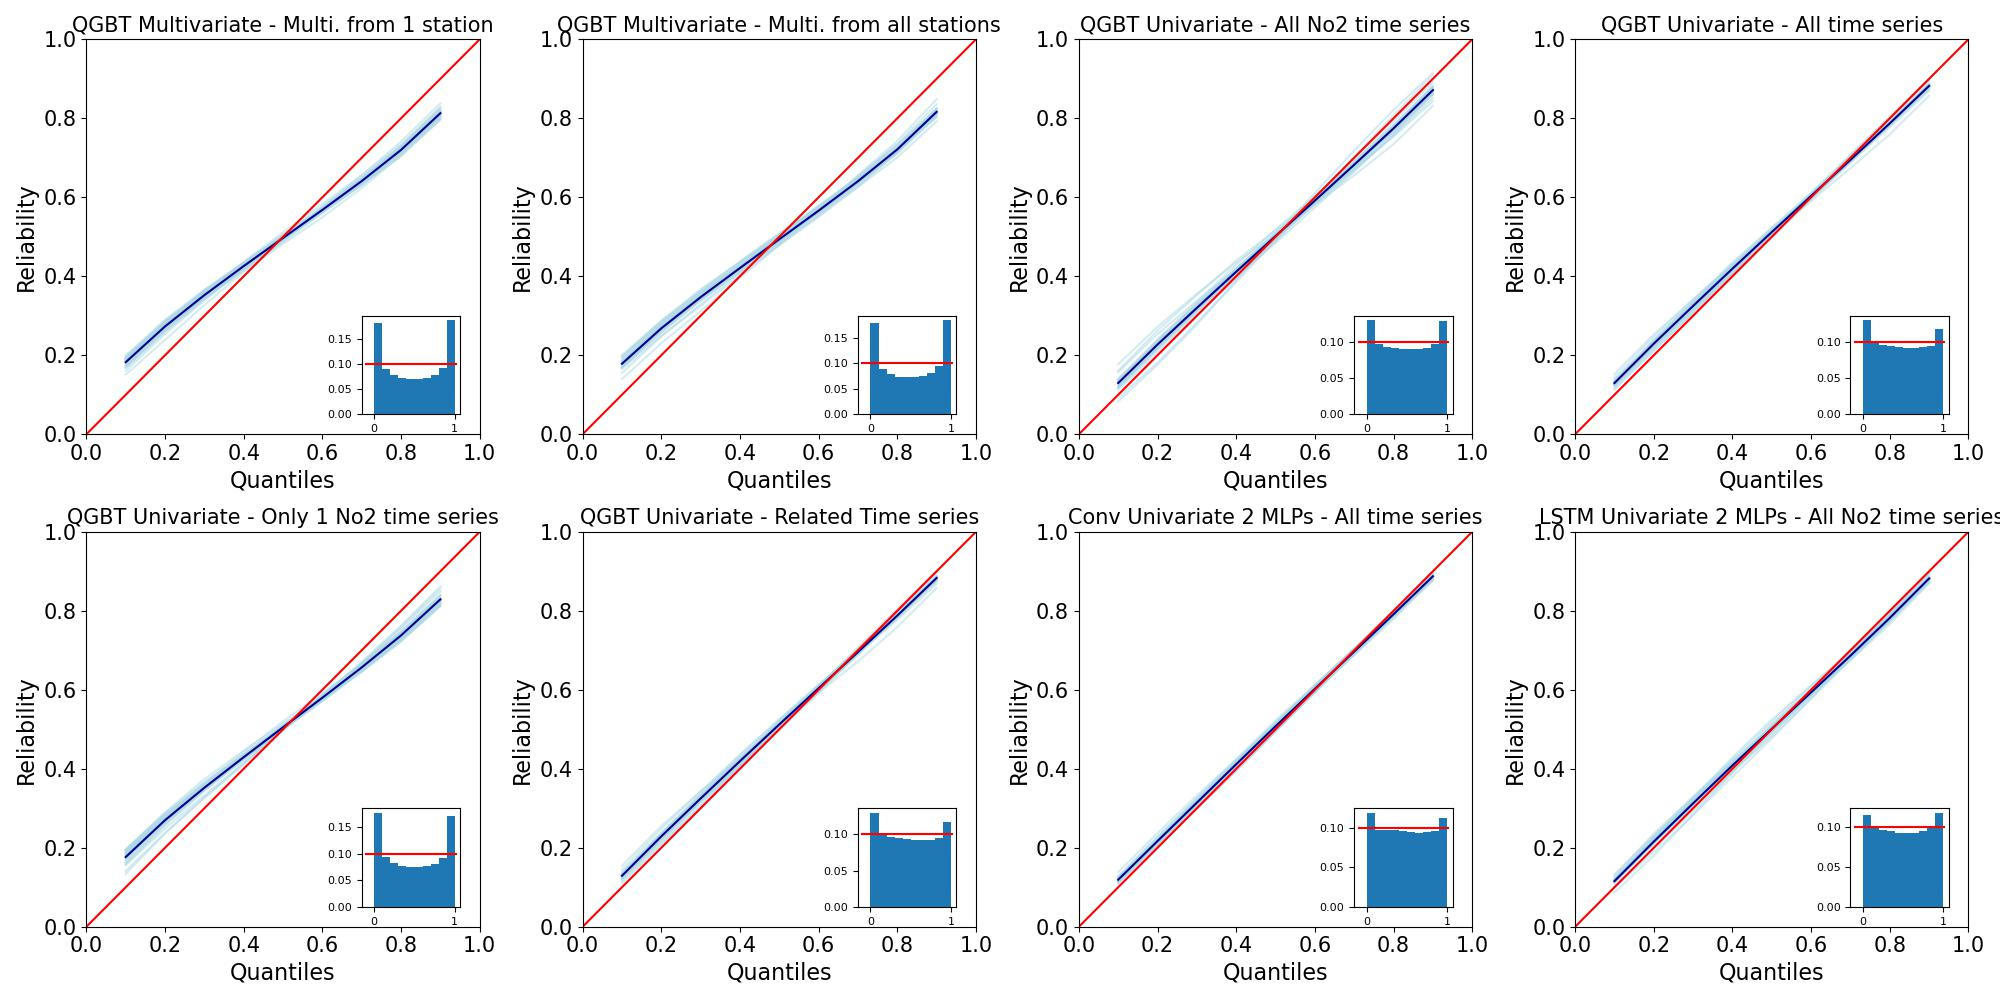
\includegraphics[width=1\textwidth]{exp2a_rel_sharp.jpg}
  \caption{Reliability and sharpness curves of the top performant experimental configurations}
  \label{fig:exp2a_rel_sharp}
\end{figure}

Reliability and sharpness diagrams (Figure \ref{fig:exp2a_rel_sharp}) for the leading experimental configurations provides further visual insights into the quality of the probabilistic forecasts. These diagrams show that the models from the QGBT configurations overfit, as shown by the sharpness histograms peaking at the extremes. This suggests their predicted distributions were often too narrow, underestimating the true uncertainty. On the contrary, the deep learning models within the top group generally exhibit better calibration, with flatter sharpness histograms and reliability curves closer to the ideal diagonal, indicating a more accurate representation of forecast uncertainty.

Training times are not directly correlated with the volume of training data (i.e., number of time series used). This is primarily attributed to the use of an early stopping mechanism, which halts training based on validation performance rather than a fixed number of epochs. However, differences are observed between model types: QGBT models generally demand longer training times compared to the deep learning models. Additionally, the Global Forecasting Model (GFM) approach presents the advantage of having to train a single model for all stations (instead of a model per station). Also, we see that the training time for a global model is shorter than training local models for each time series.

\begin{table}[h]
\centering
\begin{tabular}{lrrrrr}
\toprule
 Experimental configuration & True Positives & False Positives & Precision & Recall & F1 Score \\
\midrule
CONV M 1M SSt & 46 & 347 & 0.12 & 0.10 & 0.11 \\
LSTM M 1M ATS & 42 & 206 & 0.17 & 0.09 & 0.12 \\
CONV U 2M ANo2 & 39 & 114 & 0.25 & 0.08 & 0.13 \\
QGBT M ATS & 37 & 42 & 0.47 & 0.08 & 0.13 \\
QGBT M SSt & 35 & 49 & 0.42 & 0.07 & 0.13 \\
    CONV U 2M SNo2 & 32 & 119 & 0.21 & 0.07 & 0.10 \\
    CONV U 2M RTS & 31 & 60 & 0.34 & 0.07 & 0.11 \\
    QGBT U ATS & 31 & 44 & 0.41 & 0.07 & 0.11 \\
    QGBT U ANo2 & 29 & 36 & 0.45 & 0.06 & 0.11 \\
    CONV M 1M ATS & 24 & 49 & 0.33 & 0.05 & 0.09 \\
    QGBT U SNo2 & 24 & 37 & 0.39 & 0.05 & 0.09 \\
    QGBT U RTS & 23 & 42 & 0.35 & 0.05 & 0.09 \\
    LSTM M 1M SSt & 23 & 171 & 0.12 & 0.05 & 0.07 \\
    CONV U 2M ATS & 20 & 19 & 0.51 & 0.04 & 0.08 \\
    LSTM U 2M ANo2 & 20 & 45 & 0.31 & 0.04 & 0.08 \\
    CONV U 1M SNo2 & 17 & 576 & 0.03 & 0.04 & 0.03 \\
    LSTM U 2M RTS & 16 & 38 & 0.30 & 0.03 & 0.06 \\
    CONV U 1M ANo2 & 9 & 13 & 0.41 & 0.02 & 0.04 \\
    CONV M 2M ATS & 9 & 14 & 0.39 & 0.02 & 0.04 \\
    LSTM M 2M ATS & 9 & 13 & 0.41 & 0.02 & 0.04 \\
    CONV M 2M SSt & 8 & 12 & 0.40 & 0.02 & 0.03 \\
    LSTM U 1M ATS & 7 & 13 & 0.35 & 0.02 & 0.03 \\
    LSTM U 1M RTS & 7 & 12 & 0.37 & 0.02 & 0.03 \\
    LSTM M 2M SSt & 7 & 12 & 0.37 & 0.02 & 0.03 \\
    LSTM U 1M ANo2 & 6 & 11 & 0.35 & 0.01 & 0.03 \\
    CONV U 1M ATS & 6 & 12 & 0.33 & 0.01 & 0.03 \\
    LSTM U 1M SNo2 & 5 & 12 & 0.29 & 0.01 & 0.02 \\
    LSTM U 2M ATS & 4 & 16 & 0.20 & 0.01 & 0.02 \\
    LSTM U 2M SNo2 & 4 & 12 & 0.25 & 0.01 & 0.02 \\
    CONV U 1M RTS & 2 & 2 & 0.50 & 0.00 & 0.01 \\
\bottomrule
\end{tabular}

\caption{Performance of the different models as classifiers of peaks ((>180$\mu$g/m3)). True positives and False positives.  }
\label{tab:exp2a_classif}
\end{table}

Finally, we also measure the ability of the models to predict high-pollution events (defined as \no{} concentrations exceeding 180 $\mu g/m^3$). As mentioned in Section \ref{peak_detect}, standard classification metrics like accuracy are not valid for this due to the high class imbalance of this case. Indeed, pollution peaks are a rare event. Therefore, performance is evaluated based on the counts of True Positives (TP) and False Positives (FP), as shown in Table \ref{tab:exp2a_classif}. Configurations detecting a higher number of actual peaks (higher TPs) often did so at the cost of a disproportionately large number of false alarms (higher FPs). For instance, the Multivariate Convolutional model with 1 MLP trained on single station data (CONV M 1M SSt) identifies a relatively high number of peaks but generated numerous FPs. The Univariate Convolutional model with 2 MLPs trained on all time series (CNN U 2M ATS) offers the most balanced performance in this regard, achieving the highest ratio of TPs to FPs among all tested configurations. Overall, the F1 scores remain low across all models, showing the significant challenge of reliably forecasting the high-pollution episodes.

\subsubsection{Focus on the Transformer Models}

\begin{figure}[h!]
  \centering
  % Use a wider width since the image contains two plots
  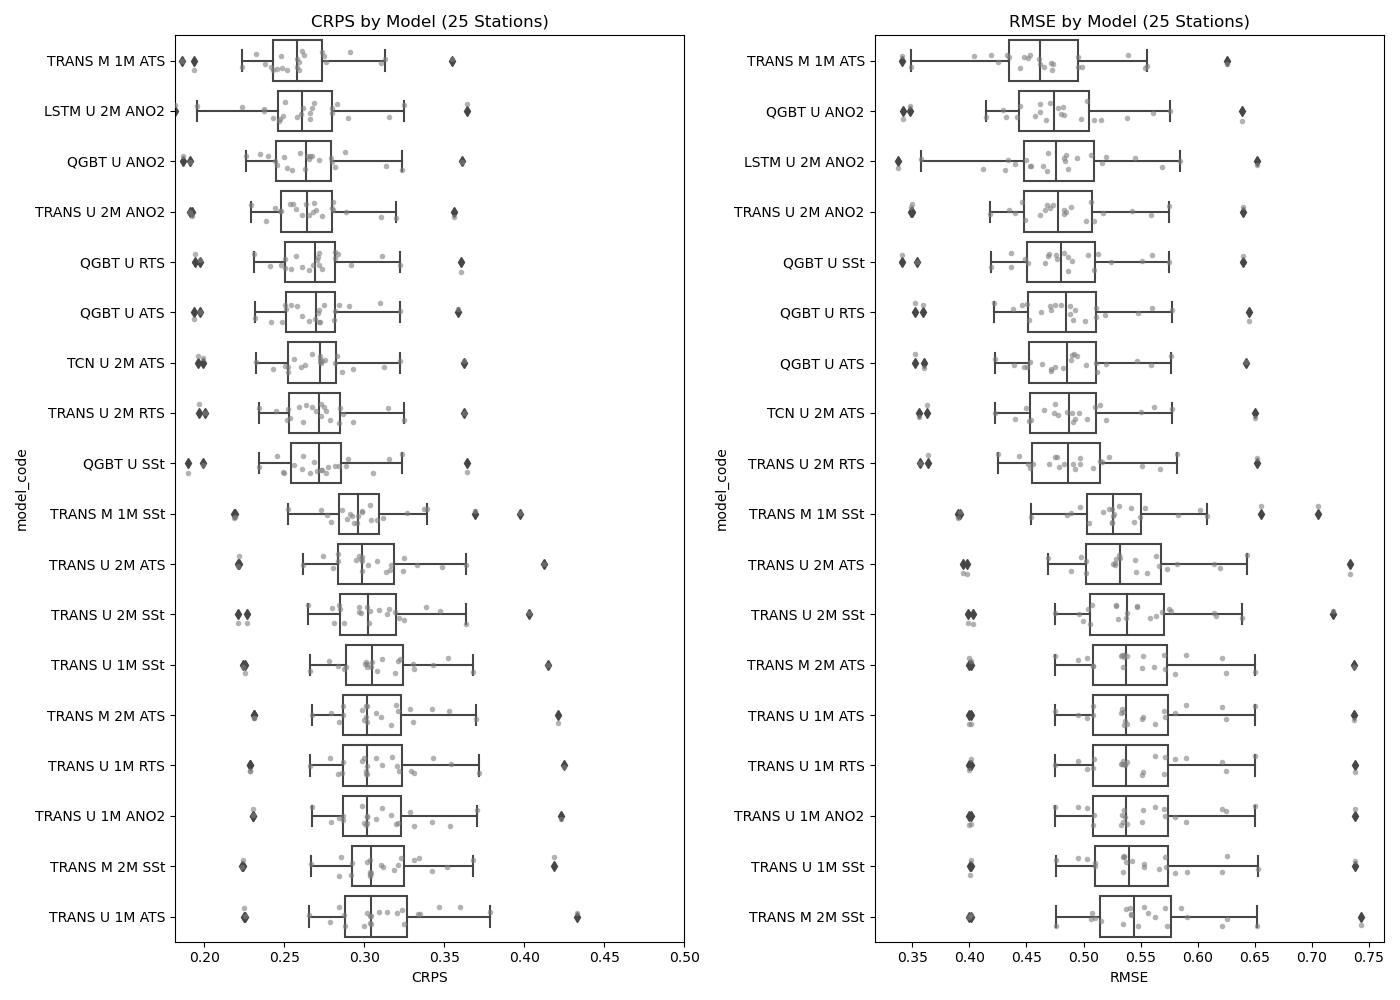
\includegraphics[width=\textwidth]{exp2b_rmse_crps.png} 
  \caption{Distribution of normalized CRPS (left) and RMSE (right) scores for each experimental configuration across all 25 stations. Models are sorted independently in each panel by their mean performance.}
  \label{fig:exp2b_rmse_crps_boxplot}
\end{figure}

The overall performance of each model configuration is summarized in Figure \ref{tab:exp2b_rmse_crps_boxplot}, which displays the distribution of CRPS and RMSE scores across all 24 stations. In these boxplots, we see the the multivariate transformer model with 1 MLP and trained on all stations (TRANS M 1M ATS) is the best performing configuration, both on CRPS and RMSE metrics. This is the only transformer configuration that surpasses the best QGBT and LSTM configuration. However, we see that this transformer configuration has a worse bias than those 2 other configurations. The other transformer configurations exhibited comparable or worse performance  than of those previous top performing configurations. 

Again, we see that for multivariate, 1 MLP configuration is better and in univariate, 2 MLPs provide better results. In the case of transformers configurations, we see that multivariate configurations provide better results (LSTM and CONV configurations provide different results).

\begin{figure}[h] 
  \centering  
  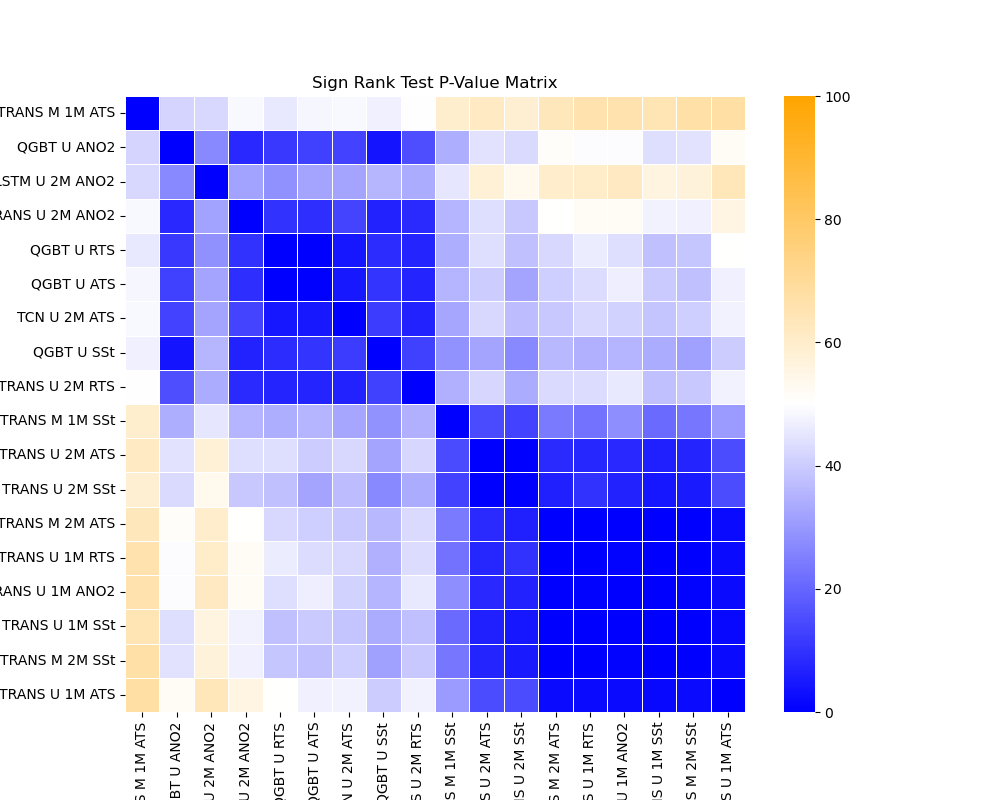
\includegraphics[width=1\textwidth]{exp2b_pairwise.png}
  \caption{Matrix of pairwise comparison between models}
  \label{fig:exp2b_pairwise}
\end{figure}

To move beyond visual inspection and formally assess the statistical significance of these observed differences, we also conducted pairwise Wilcoxon signed-rank tests between all model configurations. The resulting p-values distribution is visualized in the heatmap in Figure \ref{fig:exp2b_pairwise}. This matrix where the configurations are ordered by their Quade test ranking, reveals 3 distinct performance tiers. The top tier contains only the top transformer configuration TRANS M 1M ATS, further showing that this configuration is on his own level of performance not matched by other configurations. 

\begin{figure}[h] 
  \centering  
  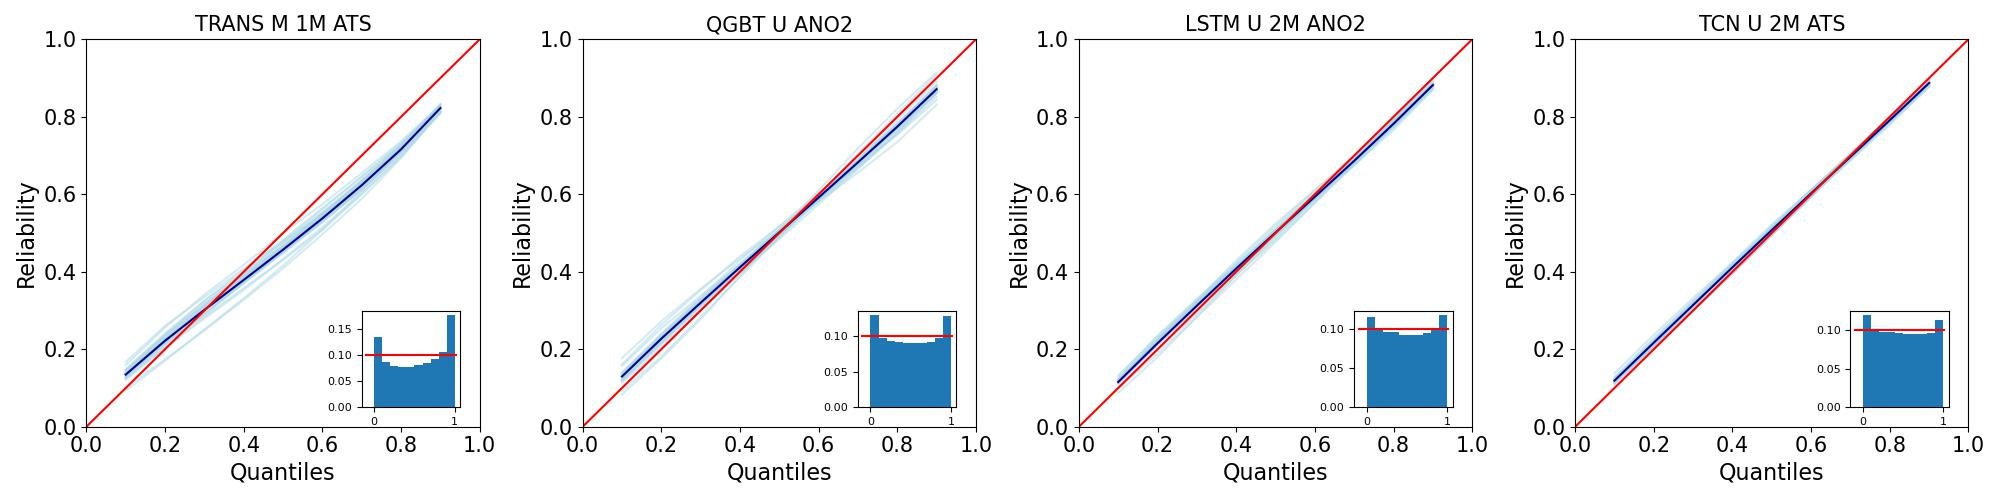
\includegraphics[width=1\textwidth]{exp2b_rel_sharp.jpg}
  \caption{Reliability and sharpness curves of the top performant experimental configurations}
  \label{fig:exp2b_rel_sharp}
\end{figure}

We also evaluate the quality of the probabilistic forecasts of the top performing configurations using reliability diagrams as shown in Figure \ref{{fig:exp2b_rel_sharp}}. As stated previously, we see that all the models tend to overfit, as we can see in the sharpness diagrams. Indeed, the long tails of the distribution are over-represented, which means that the predicted distributions are too narrow. The top performing transformer configuration (TRANS M 1M ATS) does overfit as well, even worse than the others.

\begin{table}[h]
\centering
\begin{tabular}{lrrrrr}
\toprule
 Experimental configuration & True Positives & False Positives & Precision & Recall & F1 Score \\
\midrule
TRANS M 1M ATS & 4 & 10 & 0.290000 & 0.010000 & 0.020000 \\
QGBT U ANO2 & 29 & 36 & 0.450000 & 0.060000 & 0.110000 \\
LSTM U 2M ANO2 & 20 & 45 & 0.310000 & 0.040000 & 0.080000 \\
TRANS U 2M ANO2 & 10 & 14 & 0.420000 & 0.020000 & 0.040000 \\
QGBT U RTS & 23 & 42 & 0.350000 & 0.050000 & 0.090000 \\
QGBT U ATS & 31 & 44 & 0.410000 & 0.070000 & 0.110000 \\
CONV U 2M ATS & 20 & 19 & 0.510000 & 0.040000 & 0.080000 \\
QGBT U SSt & 24 & 37 & 0.390000 & 0.050000 & 0.090000 \\
TRANS U 2M RTS & 19 & 35 & 0.350000 & 0.040000 & 0.070000 \\
TRANS M 1M SSt & 7 & 23 & 0.230000 & 0.020000 & 0.030000 \\
TRANS U 2M ATS & 5 & 7 & 0.420000 & 0.010000 & 0.020000 \\
TRANS U 2M SSt & 4 & 8 & 0.330000 & 0.010000 & 0.020000 \\
TRANS M 2M ATS & 9 & 13 & 0.410000 & 0.020000 & 0.040000 \\
TRANS U 1M RTS & 8 & 13 & 0.380000 & 0.020000 & 0.030000 \\
TRANS U 1M ANO2 & 9 & 15 & 0.380000 & 0.020000 & 0.040000 \\
TRANS U 1M SSt & 6 & 10 & 0.380000 & 0.010000 & 0.030000 \\
TRANS M 2M SSt & 8 & 11 & 0.420000 & 0.020000 & 0.030000 \\
TRANS U 1M ATS & 9 & 13 & 0.410000 & 0.020000 & 0.040000 \\
\bottomrule
\end{tabular}

\caption{Performance of the different models as classifiers of peaks ((>180$\mu$g/m3)). True positives and False positives.  }
\label{tab:exp2b_classif}
\end{table}


Finally, we assess the models' capability to predict high-pollution events. The performance is detailed on Figure \ref{tab:exp2b_classif}. We see that the top transformer configuration does not do a better job than the other configurations in this regard. There's a low number of predicted peaks, indicating most likely that the predicted distribution is narrow with a conservative long tail. On the other hand, we see that other transformer configurations that are performing worse on usual metrics do perform better on this classification task. For instance, the Univariate Transformer with 2 MLPs has a higher number of TPs with less FPs.

\section{Post-hoc calibration results}

To address the calibration of the best-performing models identified in the previous experiment, we apply several individual and combined post-hoc calibration techniques described in section \ref{exp:posthoc}: Temperature Scaling (TS), Scale Binning (SB), Quantile Mapping (QM), a simple Bias Correction (BC) and a combined Quantile Mapping followed by Scaling Binning (QM+). As outlined in the experimental design, the top-performing configurations for each architecture: LSTM U 2M ANO2, QGBT U ANO2, CONV U 2M ATS, and TRANS M 1M ATS are calibrated using a dedicated dataset comprising 5\% of the original training data. The impact of these adjustments was then evaluated on the identical test set and metrics.

The results, summarized in the performance metrics table \ref{tab:exp3_complex1} show little improvement. BC has almost no effect on the metrics and even the bias which is supposed to correct does not show great improvement. It provides the best improvement for the transformer configuration where the bias is reduced by half (from 4.32 to 2.65). QM shows much better bias correction. It succeeds to eliminate almost all bias for QGBT, LSTM and Transformer configuration and reduces it by half for the Convolutional configuration. However, this comes at the cost of degrading considerably all other metrics (almost 30\% degradation). The TS method improves very slightly the CRPS metric and leaves the rest unchanged. SB yields the same effect which shows that applying histogram binning after temperature scaling does not add any benefit to the metrics. Finally, QM+ has almost the same results than QM alone.

\begin{figure}[h] 
  \centering  
  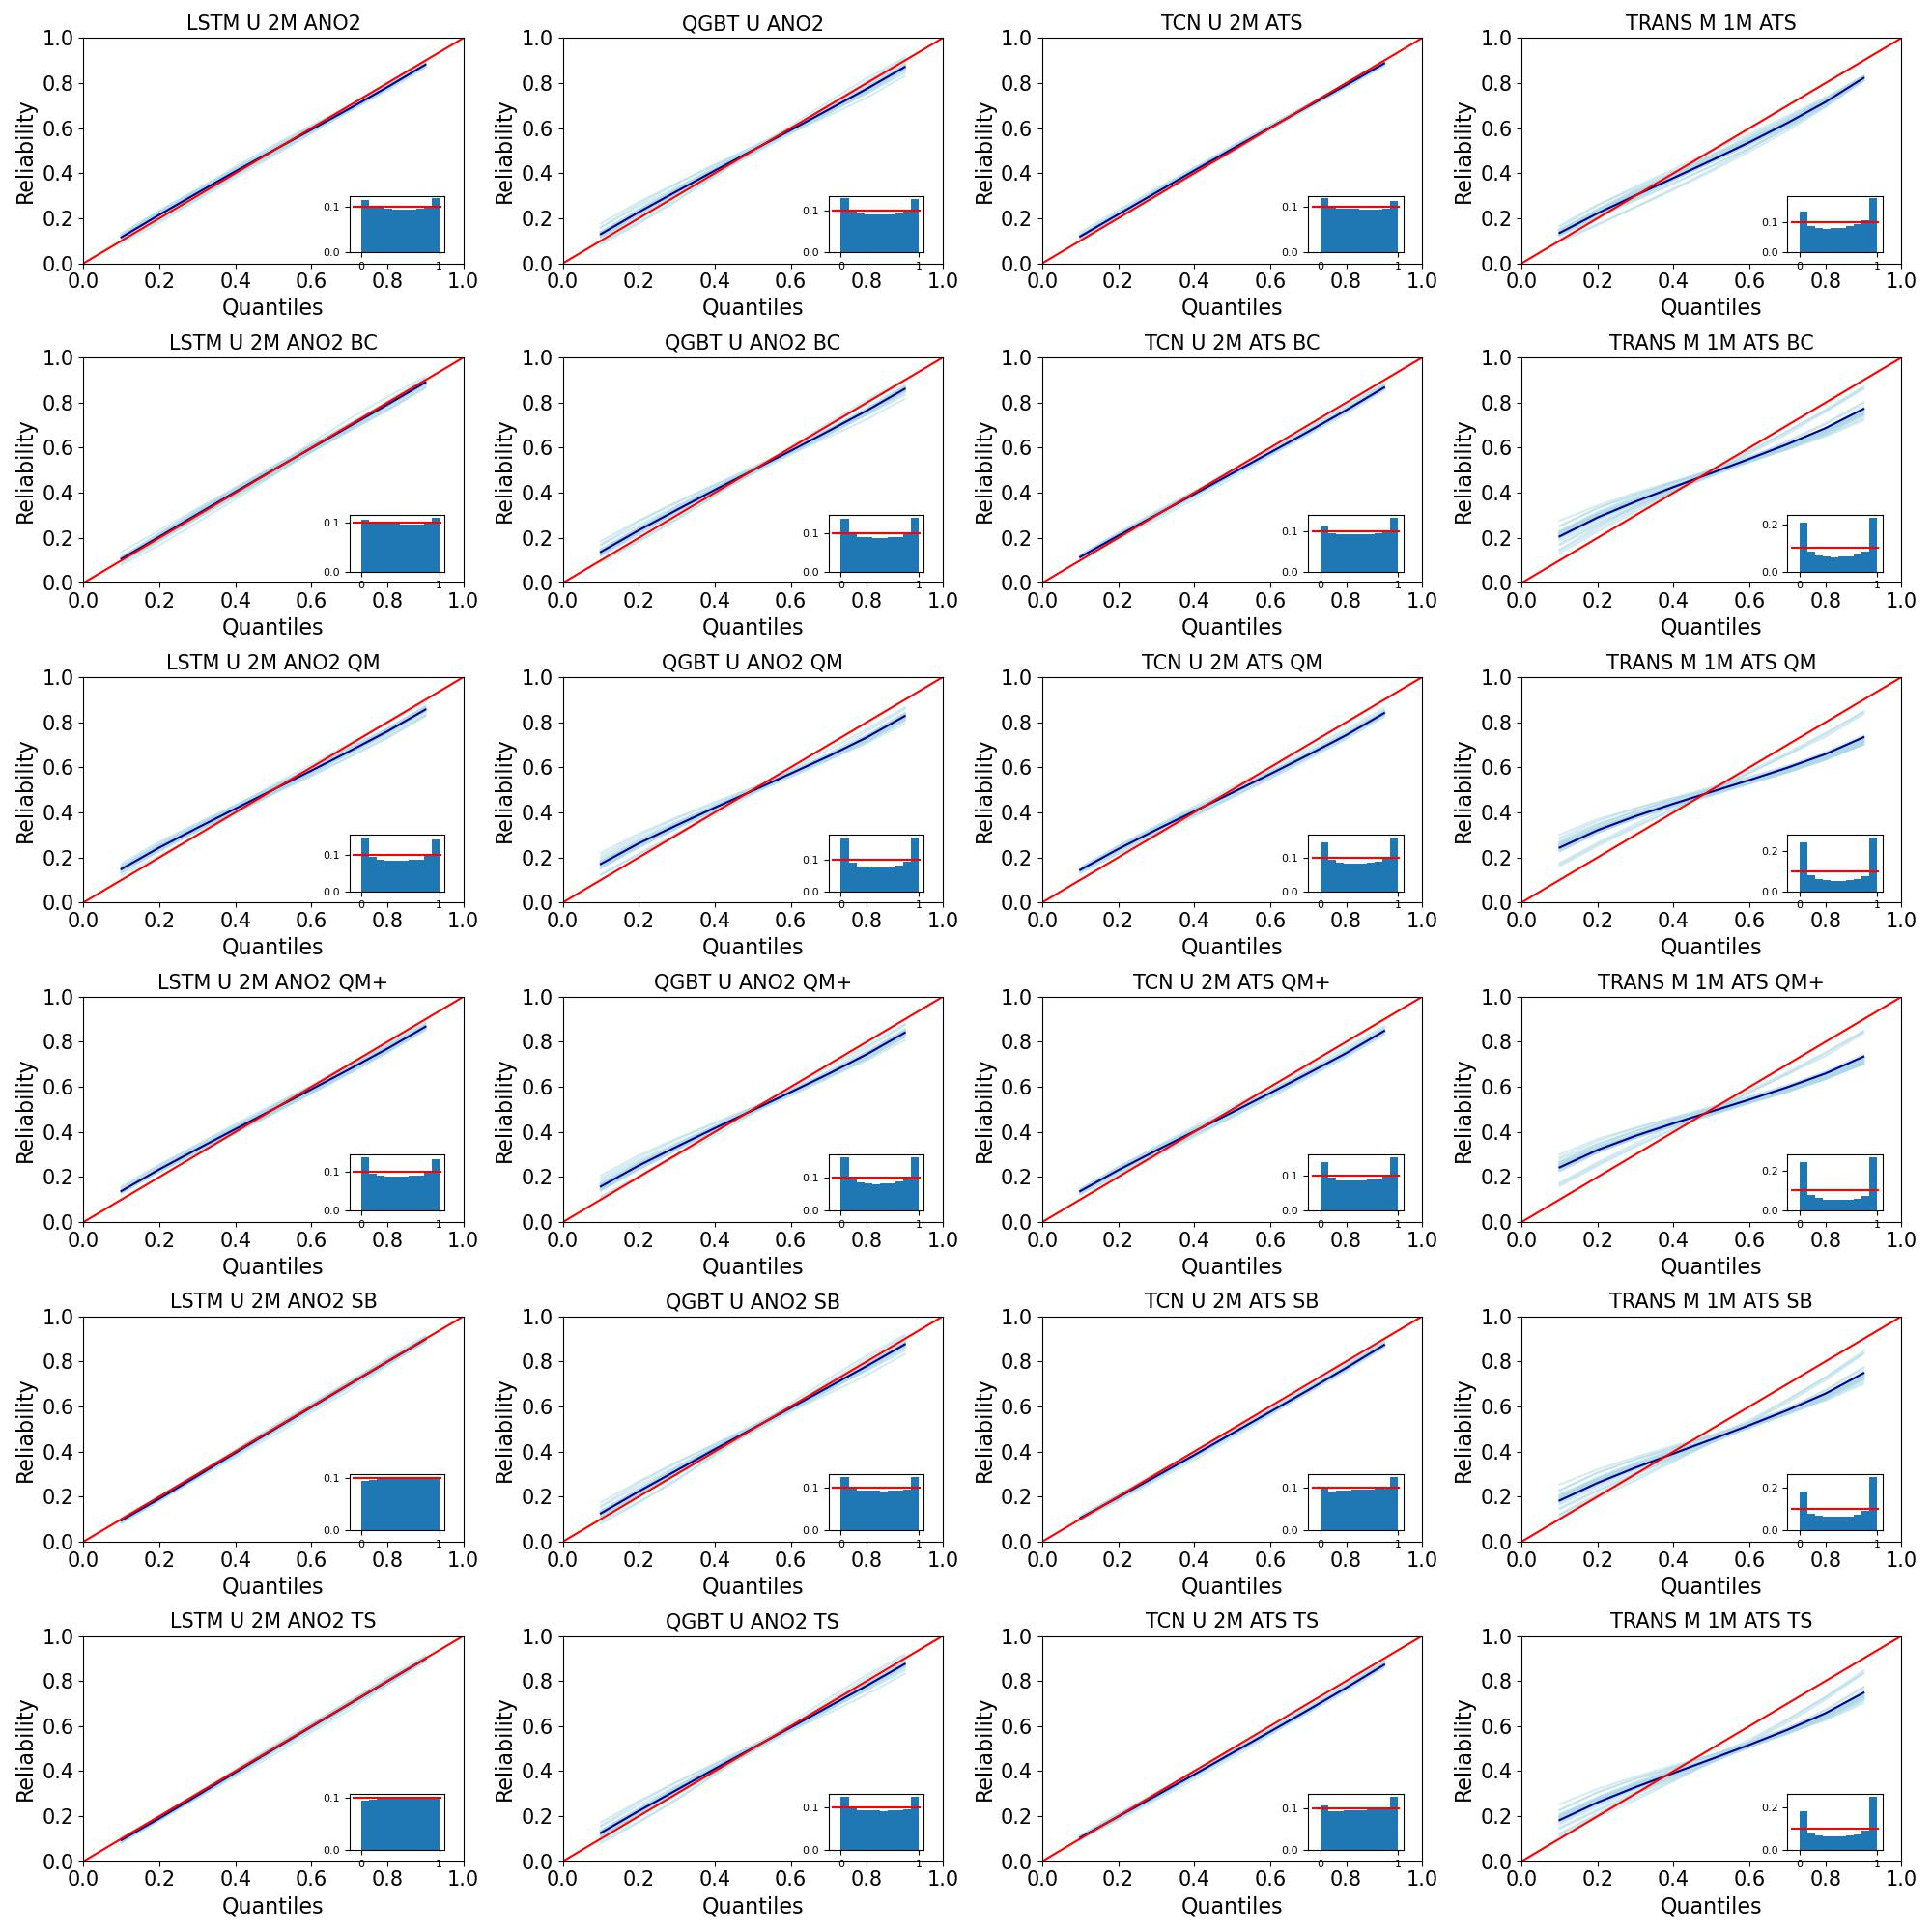
\includegraphics[width=1\textwidth]{exp3_rel_sharp.jpg}
  \caption{Reliability and sharpness curves of the calibrated  experimental configurations}
  \label{fig:exp3_rel_sharp}
\end{figure}


As previously stated in the previous experiment, the reliability and sharpness curves show that all the configurations overfit as they show that the predicted distribution is too narrow and underestimates the probability of occurrences on the long tails. First, QM and QM+ degrade the sharpness for all methods. Then, SB, TS and BC do a good job on calibrating the predictions for LSTM and CONV as we see a flatter sharpness curve. However, they have no effect on QGBT and Transformer configurations' results.  

\begin{table}[h]
\centering
\begin{tabular}{lrrrrr}
\toprule
 Experimental configuration & True Positives & False Positives & Precision & Recall & F1 Score \\
\midrule
LSTM U 2M ANO2 BC & 9 & 20 & 0.310000 & 0.020000 & 0.040000 \\
LSTM U 2M ANO2 ORIG & 21 & 43 & 0.330000 & 0.020000 & 0.040000 \\
LSTM U 2M ANO2 QM & 66 & 453 & 0.130000 & 0.140000 & 0.130000 \\
LSTM U 2M ANO2 QM+ & 66 & 454 & 0.130000 & 0.140000 & 0.130000 \\
LSTM U 2M ANO2 SB & 9 & 16 & 0.360000 & 0.020000 & 0.040000 \\
LSTM U 2M ANO2 TS & 9 & 16 & 0.360000 & 0.020000 & 0.040000 \\
QGBT U ANO2 BC & 30 & 34 & 0.470000 & 0.060000 & 0.110000 \\
QGBT U ANO2 QM & 92 & 777 & 0.110000 & 0.190000 & 0.140000 \\
QGBT U ANO2 QM+ & 92 & 780 & 0.110000 & 0.190000 & 0.140000 \\
QGBT U ANO2 SB & 31 & 37 & 0.460000 & 0.070000 & 0.110000 \\
QGBT U ANO2 TS & 31 & 37 & 0.460000 & 0.070000 & 0.110000 \\
CONV U 2M ATS BC & 12 & 13 & 0.480000 & 0.030000 & 0.050000 \\
CONV U 2M ATS QM & 63 & 330 & 0.160000 & 0.140000 & 0.150000 \\
CONV U 2M ATS QM+ & 63 & 332 & 0.160000 & 0.140000 & 0.150000 \\
CONV U 2M ATS SB & 12 & 13 & 0.480000 & 0.030000 & 0.050000 \\
CONV U 2M ATS TS & 12 & 13 & 0.480000 & 0.030000 & 0.050000 \\
TRANS M 1M ATS BC & 29 & 480 & 0.060000 & 0.060000 & 0.060000 \\
TRANS M 1M ATS ORIG & 20 & 333 & 0.060000 & 0.040000 & 0.050000 \\
TRANS M 1M ATS QM & 60 & 2172 & 0.030000 & 0.130000 & 0.040000 \\
TRANS M 1M ATS QM+ & 60 & 2172 & 0.030000 & 0.130000 & 0.040000 \\
TRANS M 1M ATS SB & 20 & 332 & 0.060000 & 0.040000 & 0.050000 \\
TRANS M 1M ATS TS & 20 & 333 & 0.060000 & 0.040000 & 0.050000 \\
\bottomrule
\end{tabular}

\caption{Performance of the different models as classifiers of peaks ((>180$\mu$g/m3)). True positives and False positives.  }
\label{tab:exp3_classif}
\end{table}

Finally, we want to measure how well those calibrated methods can predict pollution peaks (levels higher than 180$\mu g/m^3$). First, we see that the calibration methods degrade considerably all classification metrics for the transformer configuration. Then, SB and TS improve the precision of the predictions but with a worse recall. However, this is preferable as it reduces the overall number of false positives. Bias Correction brings almost the same benefits than SB and TS for CONV and QGBT configurations. Finally, the best configuration before calibration is the CONV configuration with 20 true positives and 19 false positives. With the SB, TS or BC calibration, we get the number of true positives reduced to 12 with 13 false positives. This is preferable as we keep the precision of the predictions and we reduce the number of false positives. 

\chapter{Discussion}
%No haer subsecciones para cada experimento, tiene que haber una sección global donde se discuta todo en conjunto%
This investigation into probabilistic air pollution forecasting shows an evolution of architectures (from classical machine learning models to advanced deep learning architectures with post-hoc calibration) and innovations around those. This progression has provided several key insights into what drives performance in this domain.

In this forecasting exercise, we are using lagged values to forecast the \no{} distribution. In our first experiment, we are simply feeding those values into the different models with minimal pre-processing, simply applying a logarithmic transformation. This is considered a good practice as it effectively stabilizes variance and reduces skewness. It also reduces the values and serves as a standardization step. We do not extract the seasonality nor trend. We assume there's no trend in the pollution time series and for the seasonality, we decide to have the model learn it through calendar variables as additional features in the training dataset. The classical machine learning models take the data in tabular form where the temporal order of the features is not taken into account. 

The first thing we notice with this approach is the strong correlation between lagged values and the target. This explains QLR's good performance. From the QRFL and QKNNL's better performance than QLR, we conclude that there are non-linear dynamics: a primary linear signal exists, but a significant, non-linear component remains in the residuals, which must be modeled to achieve top-tier accuracy.

QGBT is therefore the most performant model as it is able to model both components showing its inherent strength in modeling tabular data with a mix of linear and complex, non-linear relationships. Also, its architecture (additive from several trees arranged sequentially) explains why the QGBTL model, which combines a linear model and QGBT to forecast the distribution of residuals, has no better performance than the original QGBT.

In the second set of experiments, we can see the benefits of improving the forecasting process. First, regarding the pre-processing of the data, we remove the trend and seasonality of the time series through a STL decomposition. Indeed, the air quality is worsening over time with higher values of \no{} (as it is tied to human activity) and this trend need to be taken into account. Also we remove the burden of predicting the seasonality of the target variable, so the models can focus on predicting the residuals. For example, we see QGBT's average CRPS and RMSE decrease by 14\% and 12\% respectively after adding this pre-processing step.

We also introduce the use of global time series models: whereas local models are trained independently on each time series, a single global forecasting model is trained against a whole set. As mentioned previously, those display good performance on some applications and are proposed therefore for our air quality forecasting exercise. However, we could explore in this experiment how data heterogeneity affected the models’ performance. Indeed, we are testing 4 different sets of input datasets. We begin with a baseline local model trained on a single time series, then to a global model using all homogeneous NO2 series, and extend further to include related and, ultimately, all available time series. Consequently, this design enables a direct evaluation of how each model architecture responds to the introduction of varied data sources. When evaluating the different models, we see that across some of them, performance improves as more time series are added to the training set, but only up to a point for some models; beyond this, adding more series leads to a decline in performance. Table \ref{tab:exp2_perf_volume_data} shows how the performance evolves as we add more time series.


\begin{table}[h]
\centering

\begin{tabular}{lllll}
\toprule
Model & 1 time series & All No2 time series & All related time series & All time series \\
\midrule
QGBT U & 8.85 & \textbf{8.58} & 8.78 & 8.79 \\
LSTM U 2M & 10.08 & \textbf{8.60} & 10.07 & 10.11 \\
CONV U 2M & 9.24 & 9.57 & 9.05 & \textbf{8.82} \\
\bottomrule
\end{tabular}

\caption{ CRPS Performance per model and input training data. }
\label{tab:exp2_perf_volume_data}
\end{table}

This shared vulnerability highlights a fundamental challenge in global forecasting model design: the conflict between leveraging training data volume and maintaining data coherence. Figures \ref{fig:evo_ts1}, \ref{fig:evo_ts2}, \ref{fig:evo_ts3}, \ref{fig:evo_ts4}, \ref{fig:evo_ts5}, \ref{fig:evo_ts6}, \ref{fig:evo_ts7} show the daily evolution of the different time series after pre-processing and the different values and dynamics of those. We can see in the figures that the time series can be very different. We try to solve this issue with the related time series group, which is created by clustering time series through features detailed in this article \cite{bandara_forecasting_2020}. This article investigates how performance increases when using similar time series as training input. However, we see in our case that homogeneity needs to be higher in order to get to an optimal performance.

As we can see in table \ref{tab:exp2_perf_volume_data}, QGBT, LSTM and CONV's performance in a global forecasting model setup is maximized when trained with all the \no{} time series from all the stations and degrades when exposed to more heterogeneous input training data. While the outcome is the same, the underlying reason for this sensitivity is unique to the core mechanics of each model. 
For the QGBT model, the performance degradation originates from the nature of its decision tree-based learning. When trained on a heterogeneous feature space, the model is forced to evaluate split points on different variables, for example having to adapt those thresholds on a normalized temperature feature with one on a normalized NO2 feature. This creates unstable decision boundaries. Furthermore, the inclusion of numerous external variables reduces the signal-to-noise ratio, making it harder for the model to identify the most predictive features and increasing the risk of learning spurious correlations. Conversely, on the more homogeneous dataset with all the \no{} time series, all features are directly comparable, allowing the model to learn meaningful rules.
The LSTM architecture suffers from a different form of representational interference due to its hidden state. The LSTM's core function is to compress the sequence history into a hidden state, but the rules for updating this state are highly dependent on the input data's dynamics. For example, a single set of learned gates struggles to create a meaningful hidden state for both spiky, event-driven pollution series and slow, smooth meteorological series. This forces the model to learn a compromised, underfit representation that is not optimal for any single task. When trained only on the homogeneous \no{} time series, the LSTM can specialize and learn to generate a coherent representation of the \no{} sequence of values.

The CONV architecture, however, exhibits a fundamentally different and more robust response to data heterogeneity. Its reliance on convolutional kernels, which function as localized pattern detectors rather than holistic state summarizers, provide this resilience. Each kernel learns to identify a specific pattern within the time series, such as a sharp spike, a slow dip, or a noisy plateau. And more importantly, a kernel trained to recognize a specific shape is indifferent to the absolute values of the data, as its activation depends only on the relative structure.  Therefore when a CONV is trained on a diverse dataset with all the time series, it does not suffer from the representational interference seen in other models. Instead, it benefits by building a rich and generalized library of patterns. For instance, it can learn the characteristic sharp spike pattern from the \no{} or \ot{}, or the slow, rolling dip from diurnal temperature cycles. This ability to extract universal, value-agnostic features allows the CONV to effectively leverage all the information provided by a wide range of time series, turning data heterogeneity from a liability into an asset for model training.

Finally, for future developments, we could envision increasing the homogeneity across time series with additional pre-processing. For instance, we were not applying Min-Max standardization which means that different time series had different absolute values (although the logarithm transformation is reducing the differences). Also the seasonal pre-processing could be different for each time series. Finally we could create an input dataset with sensor data (\no{}, \ot{}, \pmtwo{} and \pmten{}) as those time series are similar.

Despite existing literature recommending simultaneous use of time series for air pollution forecast \citep{rakholia_multi-output_2023}, a critical finding was that multivariate inputs generally degraded the performance of LSTM and CONV models when forecasting \no{}. This counterintuitive result suggests that the additional pollutant variables may introduce more noise than signal, making it difficult for these models to disentangle the specific dynamics of \no{}. The main reason we have this result is that the LSTM and CONV models are not able to leverage the additional information. This finding highlights that more data is not always better. Also, other models like QGBT handle the multivariate inputs more gracefully and just filtered out information but was not able to leverage it. This means that the additional information did not degrade considerably the results, but at the same time did not provide better performance.

Also, the comparison of metrics between QGBT and those deep learning models (LSTM and CONV) did not reveal a clear advantage for the latter. Despite their design for sequential data, LSTM and CONV models did not consistently outperform QGBT. We also found in the literature instances of tree based model overtaking deep learning ones \citep{wesselkamp_advances_2025}. This result may seem surprising given the success of CONV and specially LSTM in many sequence modeling tasks, but those results have already been reported on other forecasting problems \citep{wesselkamp_advances_2025}.

However, the transformer architecture is able to successfully leverage multivariate inputs to achieve superior performance. In the univariate setting, the transformer model is not able to achieve the same level of performance than LSTM and CONV. However on the multivariate configuration, the transformer configuration using all air quality stations data outperforms all the other models. This shows that the model is specifically designed for complex multivariate setting. This also highlights the primary advantage of its self-attention mechanism. Unlike LSTMs, which process information sequentially, Transformers can dynamically weigh the importance of all input variables at every time step. This allows the model to effectively identify which combination of features is most relevant for the \no{} forecast, leading to the best overall CRPS and RMSE scores.

However, this good performance also reveal that the models tend to overfit. Metrics like CRPS reward models that perform well on average, but the reliability diagrams consistently revealed that the top-performing models on these metrics, particularly QGBT and the Transformer, produced overly narrow and overconfident predictive distributions. We can see in those diagrams how many of the actual observations fall on the edges of the forecasted distribution. Upon visual inspection of the evolution of the forecast in figures \ref{fig:evo_pred1} and \ref{fig:evo_pred2}, we can also see how the QGBT and specially Transformer models forecast distribution that are too narrow. 

\begin{figure}[h]
  \centering  
  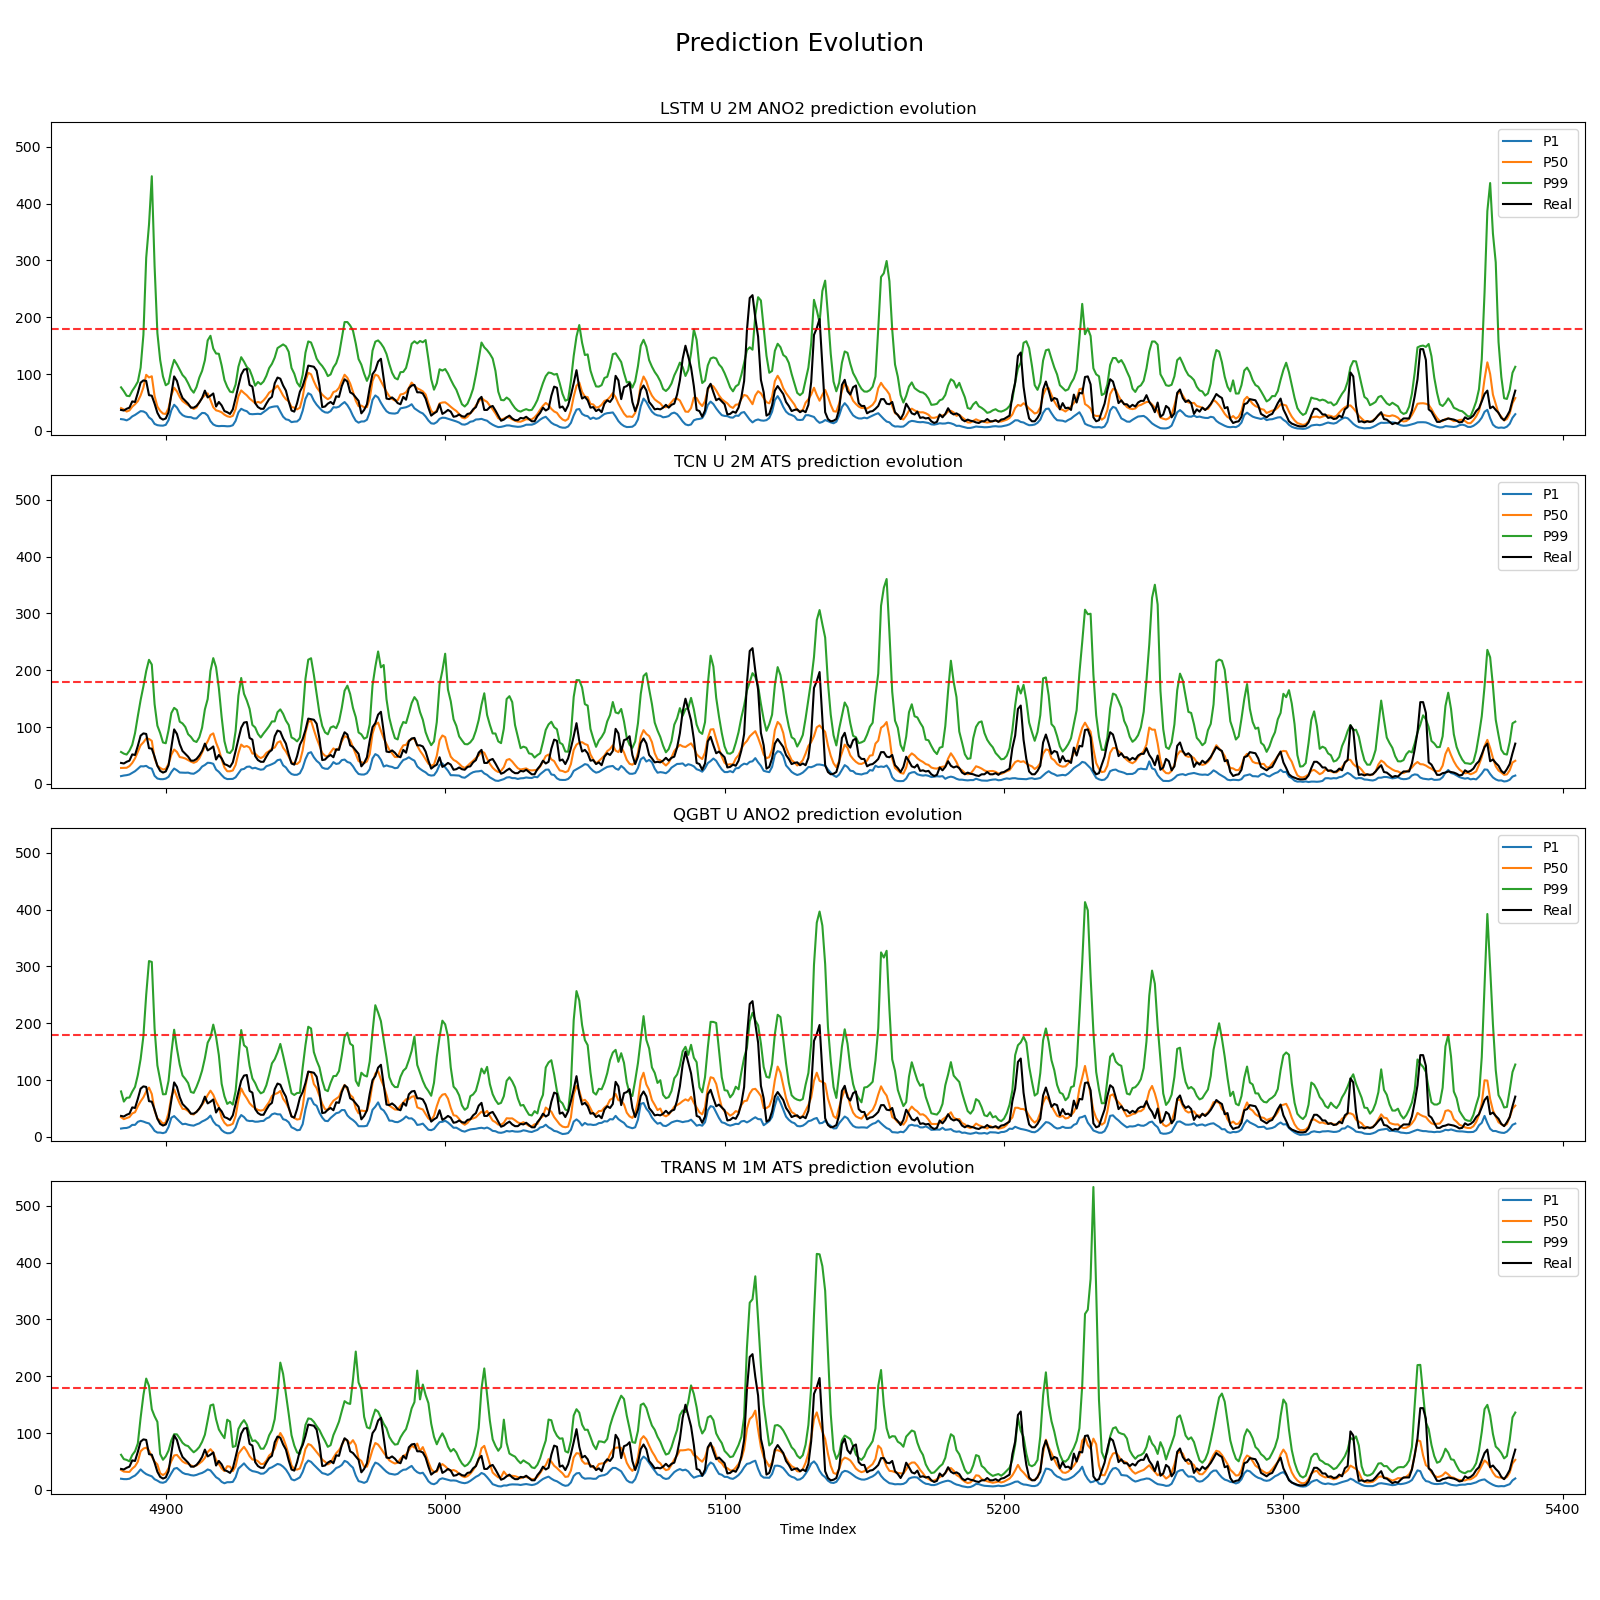
\includegraphics[width=\textwidth]{predevo1.png}
  \caption{Evolution of the forecasted probability distribution in station '28079008' for the 4 top performing models.}
  \label{fig:evo_pred1}
\end{figure}

\begin{figure}[h]
  \centering  
  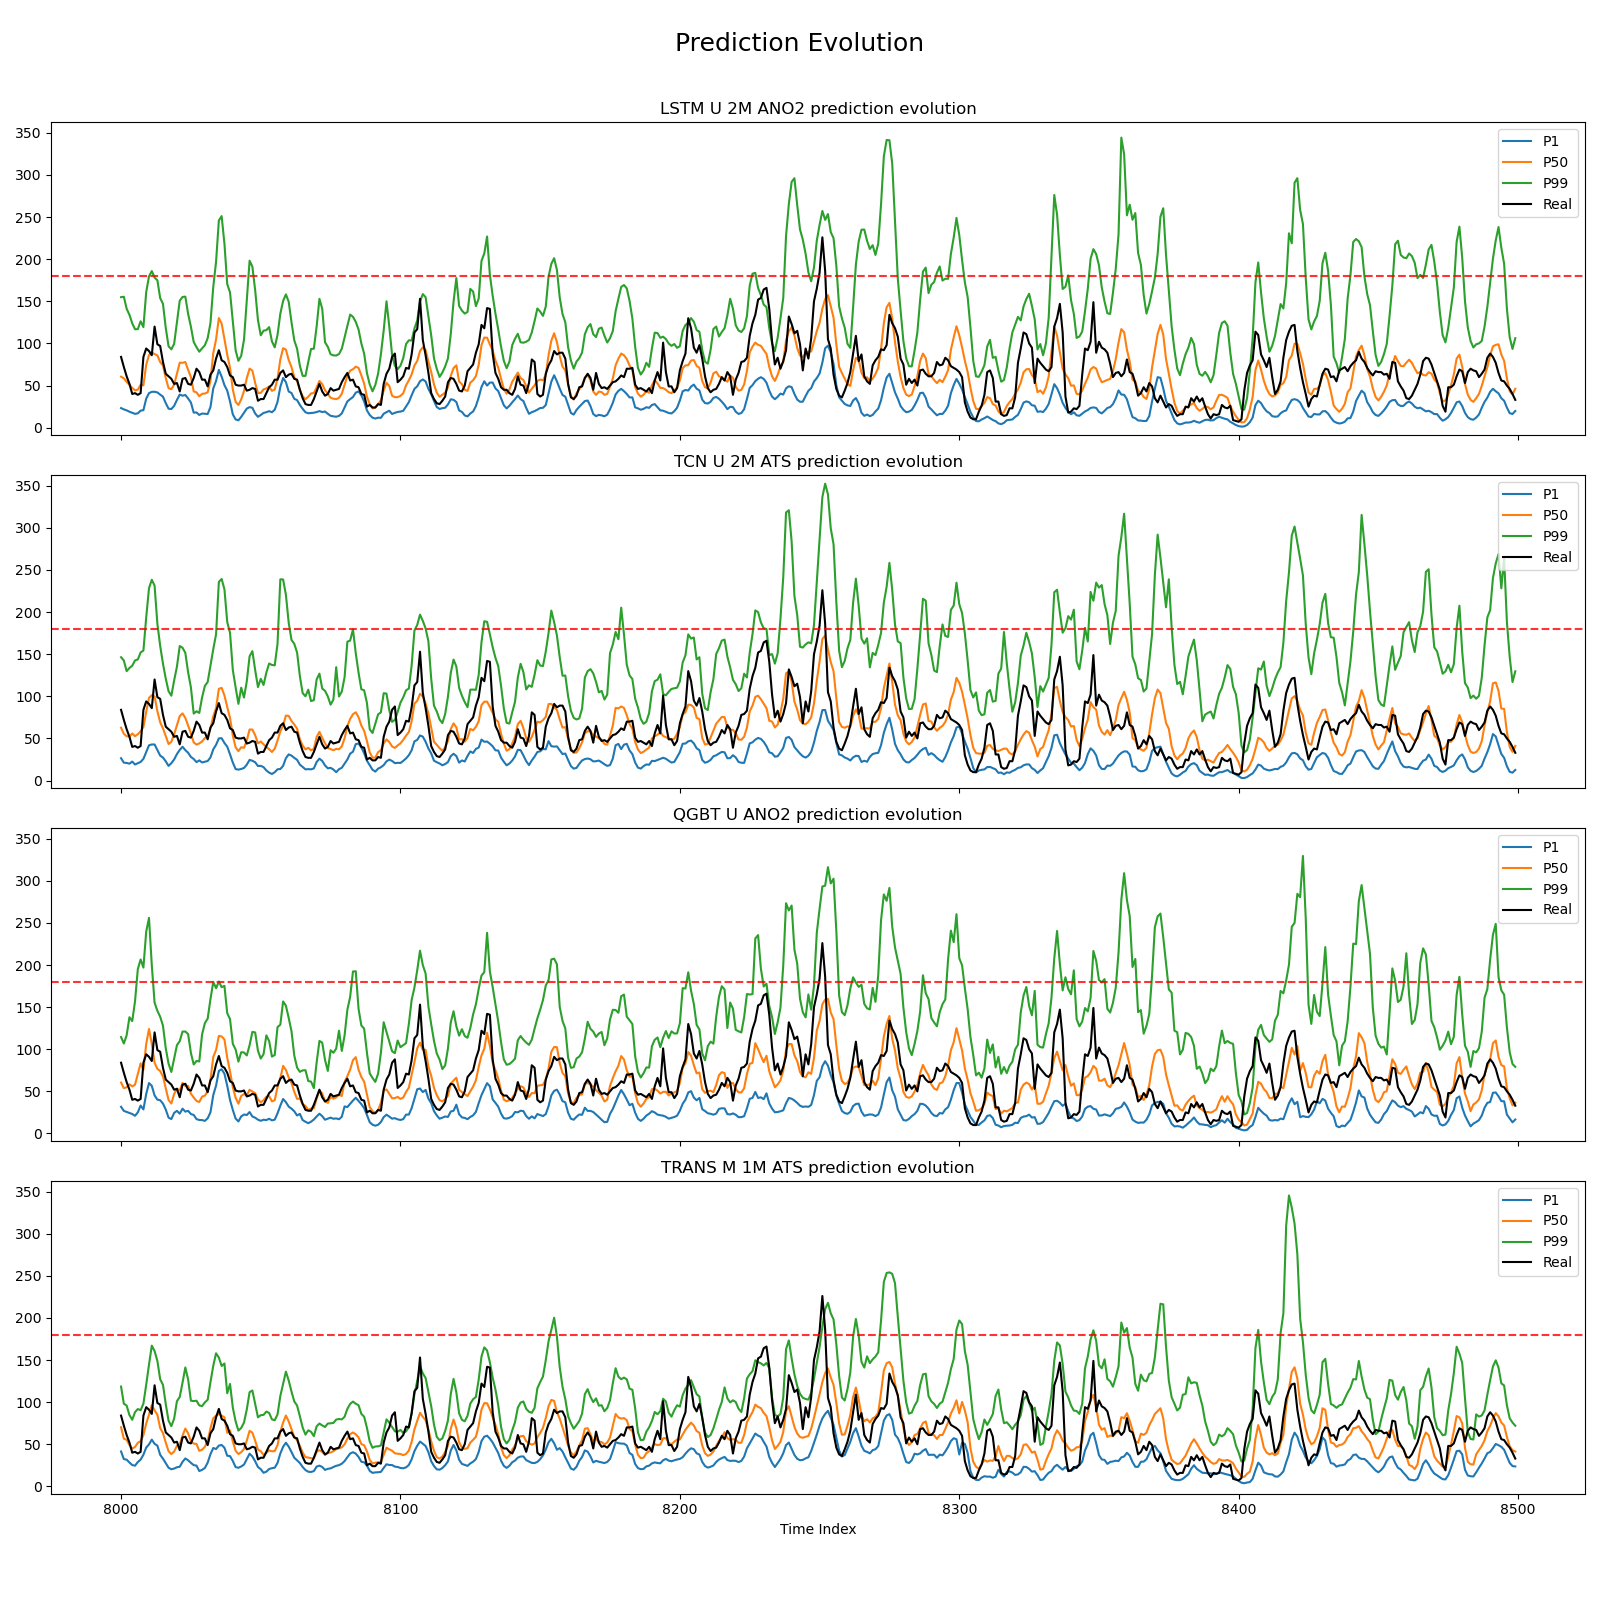
\includegraphics[width=\textwidth]{predevo2.png}
  \caption{Evolution of the forecasted probability distribution in station '28079055' for the 4 top performing models.}
  \label{fig:evo_pred2}
\end{figure}

In order to address this underestimation of the uncertainty, we apply the previously described post-hoc calibration techniques. However, this experiment shows the difficulty in correcting the probabilistic outputs of the models. As we are predicting the parameters of a distribution, our calibration efforts go towards the parameters of such forecasted distribution: the mean and the standard deviation of the Gaussian distribution. Bias Correction (BC) and Quantile Mapping (QM) address the mean of the distribution. Temperature Scaling (TS) and Scale Binning (SB) focuses on the standard deviation. Quantile Mapping followed by Scaling Binning tries to address both parameters (QM+).

We see that BC is insufficient, as it applies a constant shift without addressing distributional shape. On the other hand, QM effectively corrects the bias but all the other metrics get degraded. TS and SB provide slight improvements, particularly for the LSTM and CONV models, by re-scaling the variance. Their failure to meaningfully calibrate the QGBT and Transformer models suggests that the lack of calibration in these top-tier architectures can not be easily corrected with a simple scaling technique. Finally QM+ does not work well and degrades performance still. 

Basically, we see that no post-hoc fix can easily correct a model that overfits and learns the training data's noise too well. Therefore, we see that this would need to be addressed during training, using for example different regularization techniques. We could as well apply a higher weight to errors around the peak values to enforce correct probability estimation on the long tail of the forecasted distribution. Nevertheless, we can still evaluate the usefulness of the calibration techniques on the task of forecasting high-pollution peaks.

Indeed, we see a significant disconnect between standard performance metrics and this practical task. This underestimation of uncertainty means these models are less likely to assign significant probability to rare events, causing them to miss many actual peaks. This shows the  difficulty of forecasting in a high-imbalance context, where models can achieve excellent overall scores while failing at this specific task as it involves rare events. 

The analysis of the performance of the peak detection task for calibrated models (as seen in table \ref{tab:exp3_classif}) reveals a different hierarchy of models, with the uncalibrated multivariate Transformer and the calibrated CONV emerging as the most effective. 

The Transformer's overfit makes it underestimate the uncertainty and therefore provides very conservative peak detection. However, this is preferred as it provides fewer costly false negatives. More surprisingly, the calibrated CONV demonstrates exceptional capability, achieving the best ratio of true positives to false positives. We can speculate that the reason for this performance is that it is able to train with all the time series and could learn from more data than the other models. However, its architecture is not able to extract enough learning patterns to outperform the transformer. Also, the post-hoc calibration likely refines the model and reduces the number of false positives. Nevertheless, while these models represent a significant step forward, the overall low recall rates indicate that reliable peak forecasting remains a challenge requiring further research.


\chapter{Conclusion}
%No haer subsecciones para cada experimento, tiene que haber una sección global donde se discuta todo en conjunto%
This research is an investigation into probabilistic air pollution forecasting, progressing from classical machine learning methods to advanced deep learning architectures and post-hoc calibration techniques. The objective is to design and implement machine learning models that not only provide accurate probabilistic forecasts of Nitrogen Dioxide (\no{}) levels, which are critical for informing high-stakes decisions such as the activation of public health protocols. 

Our initial exploration of classical machine learning models establishes Quantile Gradient Boosted Trees (QGBT) as the best model demonstrating its strength in learning the complex linear and non-linear dynamics. The transition to deep learning architectures, coupled with the adoption of better pre-processing techniques and Global Forecasting Models (GFMs), reveal several important insights. First, deseasoning and detrending via STL decomposition make the task easier for the forecasting models. Second, the performance of QGBT, LSTM, and Transformer models is optimal when trained on homogeneous univariate datasets of \no{} time series, but degrades when exposed to more diverse data (like meteorological features). In contrast, the Convolutional Neural Network (CONV) architecture demonstrates superior robustness against this. Also while multivariate input data often introduced more noise than signal for LSTM and CONV models, they are indispensable for the Transformer. The self-attention architecture enables the Transformer to learn from multiple simultaneous time series, allowing it to outperform all other tested configurations. 

However, all the top performing models were overfit as we could see in the reliability and sharpness diagrams \ref{fig:exp2b_rel_sharp} or the evolution of predictions \ref{fig:evo_pred1} \ref{fig:evo_pred2}. Our subsequent experiments with post-hoc calibration techniques offer marginal improvements for the better-calibrated LSTM and CONV models, and fail to correct the Transformer and QGBT predictions, suggesting the issue must be addressed during training rather than with post-hoc fixes. This disconnect between standard metrics and peak detection provide an important insight: the "best" model is context-dependent, and optimizing for some metrics like CRPS does not guarantee the best results on all applications. 

Future research should therefore focus on better techniques during training adapted to the objective of identifying pollution peaks. This could be achieved through specific regularization techniques and custom loss functions designed to directly enforce calibration during training, particularly for rare events. We could as well work on the combination of models either through stacking or mixture of experts architectures. 

\newgeometry{top=1cm, bottom=1cm, left=2cm, right=2cm}

\begin{landscape}
\begin{table}[h]
\centering

\begin{tabular}{lrrrrrrrrrr}
\toprule
Experimental configuration & CRPS & RMSE & MAE & BIAS & CORR & CRPS(norm) & RMSE(norm) & MAE(norm) & BIAS(norm) & CORR(norm) \\
\midrule
QGBT U A\no & 8.58 & 17.9 & 12 & 2.62 & 0.746 & 0.263 & 0.476 & 0.367 & -0.004 & 0.492 \\
LSTM U 2M A\no & 8.6 & 18.2 & 12.1 & 2.69 & 0.737 & 0.262 & 0.479 & 0.369 & 0 & 0.496 \\
QGBT U RTS & 8.78 & 18.2 & 12.3 & 2.12 & 0.737 & 0.267 & 0.484 & 0.374 & -0.014 & 0.467 \\
QGBT U ATS & 8.79 & 18.3 & 12.3 & 2.14 & 0.735 & 0.267 & 0.484 & 0.374 & -0.014 & 0.464 \\
QGBT M SSt & 8.71 & 17.7 & 12 & 2.71 & 0.755 & 0.269 & 0.476 & 0.368 & -0.001 & 0.491 \\
CONV U 2M ATS & 8.82 & 18.3 & 12.4 & 2.57 & 0.734 & 0.269 & 0.486 & 0.376 & -0.008 & 0.456 \\
QGBT M ATS & 8.74 & 17.7 & 12 & 2.77 & 0.754 & 0.269 & 0.478 & 0.37 & -0.001 & 0.485 \\
QGBT U S\no & 8.85 & 18.1 & 12.2 & 2.56 & 0.74 & 0.271 & 0.482 & 0.371 & -0.007 & 0.474 \\
CONV U 2M RTS & 9.05 & 18.7 & 12.6 & 2.4 & 0.723 & 0.275 & 0.494 & 0.383 & -0.009 & 0.439 \\
LSTM M 1M ATS & 9.27 & 18.5 & 12.5 & -0.439 & 0.741 & 0.28 & 0.49 & 0.375 & -0.066 & 0.509 \\
LSTM U 2M RTS & 9.27 & 19.2 & 13 & 2.71 & 0.704 & 0.281 & 0.503 & 0.395 & -0.01 & 0.393 \\
CONV U 2M S\no & 9.24 & 18.9 & 12.7 & 2.17 & 0.719 & 0.283 & 0.504 & 0.39 & -0.009 & 0.436 \\
CONV U 2M A\no & 9.57 & 19.3 & 13 & 2.61 & 0.704 & 0.291 & 0.512 & 0.395 & 0.007 & 0.421 \\
LSTM U 2M S\no & 9.67 & 19.8 & 13.6 & 3.43 & 0.682 & 0.297 & 0.531 & 0.417 & 0 & 0.25 \\
LSTM M 1M SSt & 9.87 & 20 & 13.6 & 2.48 & 0.685 & 0.301 & 0.531 & 0.415 & -0.007 & 0.32 \\
CONV M 1M ATS & 10 & 18.4 & 12.6 & 2.08 & 0.73 & 0.306 & 0.499 & 0.386 & -0.013 & 0.455 \\
CONV M 2M ATS & 10.1 & 20.5 & 14.1 & 3.37 & 0.66 & 0.308 & 0.546 & 0.432 & 0.012 & 0.067 \\
CONV M 2M SSt & 10.1 & 20.4 & 14.1 & 3.03 & 0.66 & 0.307 & 0.547 & 0.432 & 0.001 & 0.005 \\
LSTM M 2M ATS & 10.1 & 20.4 & 14.1 & 2.91 & 0.66 & 0.308 & 0.546 & 0.432 & -0.001 & 0.073 \\
CONV U 1M S\no & 23.5 & 21.2 & 14.7 & 1.92 & 0.66 & 0.331 & 0.557 & 0.441 & -0.019 & 0.008 \\
LSTM U 1M RTS & 10.1 & 20.5 & 14.1 & 3.38 & 0.66 & 0.308 & 0.547 & 0.432 & 0.012 & -0 \\
CONV U 1M A\no & 10.2 & 20.4 & 14.1 & 2.92 & 0.66 & 0.308 & 0.546 & 0.432 & -0.001 & 0.212 \\
LSTM U 1M S\no & 10.1 & 20.5 & 14.1 & 3.13 & 0.66 & 0.308 & 0.547 & 0.433 & 0.005 & -0.02 \\
LSTM U 1M A\no & 10.1 & 20.5 & 14.1 & 3.6 & 0.66 & 0.308 & 0.547 & 0.432 & 0.019 & -0.031 \\
LSTM M 2M SSt & 10.1 & 20.5 & 14.1 & 3.27 & 0.659 & 0.308 & 0.548 & 0.433 & 0.01 & 0.003 \\
CONV M 1M SSt & 10.3 & 19.4 & 13.1 & 1.48 & 0.715 & 0.312 & 0.512 & 0.396 & -0.005 & 0.448 \\
CONV U 1M ATS & 10.1 & 20.5 & 14.1 & 3.42 & 0.66 & 0.31 & 0.547 & 0.432 & 0.014 & 0.047 \\
LSTM U 1M ATS & 10.1 & 20.4 & 14.1 & 3.2 & 0.66 & 0.311 & 0.546 & 0.432 & 0.007 & -0.024 \\
CONV U 1M RTS & 10 & 20.7 & 14.1 & 5.31 & 0.66 & 0.31 & 0.551 & 0.435 & 0.072 & 0.082 \\
LSTM U 2M ATS & 10.5 & 20.1 & 13.8 & 3.5 & 0.671 & 0.313 & 0.537 & 0.423 & 0.008 & 0.19 \\
\bottomrule
\end{tabular}

\caption{Average performance of the different experimental configurations across all stations.}
\label{tab:exp2a_complex1}
\end{table}

\end{landscape}
\restoregeometry


\newgeometry{top=1cm, bottom=1cm, left=2cm, right=2cm}

\begin{landscape}
\begin{table}[h]
\centering

\begin{tabular}{lrrrrrrrrrr}
\toprule
Experimental configuration & CRPS & RMSE & MAE & BIAS & CORR & CRPS(norm) & RMSE(norm) & MAE(norm) & BIAS(norm) & CORR(norm) \\
\midrule
TRANS M 1M ATS & 8.39 & 17.5 & 11.7 & 3.82 & 0.767 & 0.258 & 0.465 & 0.359 & 0.03 & 0.535 \\
QGBT U ANO2 & 8.58 & 17.9 & 12 & 2.62 & 0.746 & 0.263 & 0.476 & 0.367 & -0.004 & 0.492 \\
LSTM U 2M ANO2 & 8.6 & 18.2 & 12.1 & 2.69 & 0.737 & 0.262 & 0.479 & 0.369 & 0 & 0.496 \\
TRANS U 2M ANO2 & 8.63 & 18.2 & 12.2 & 3.34 & 0.741 & 0.264 & 0.48 & 0.372 & 0.007 & 0.478 \\
QGBT U RTS & 8.78 & 18.2 & 12.3 & 2.12 & 0.737 & 0.267 & 0.484 & 0.374 & -0.014 & 0.467 \\
QGBT U ATS & 8.79 & 18.3 & 12.3 & 2.14 & 0.735 & 0.267 & 0.484 & 0.374 & -0.014 & 0.464 \\
CONV U 2M ATS & 8.82 & 18.3 & 12.4 & 2.57 & 0.734 & 0.269 & 0.486 & 0.376 & -0.008 & 0.456 \\
QGBT U SSt & 8.85 & 18.1 & 12.2 & 2.56 & 0.74 & 0.271 & 0.482 & 0.371 & -0.007 & 0.474 \\
TRANS U 2M RTS & 8.89 & 18.6 & 12.5 & 3.02 & 0.726 & 0.27 & 0.489 & 0.379 & 0.005 & 0.448 \\
TRANS M 1M SSt & 9.64 & 19.9 & 13.6 & 3.97 & 0.687 & 0.298 & 0.531 & 0.421 & 0.019 & 0.269 \\
TRANS U 2M ATS & 9.86 & 20.2 & 13.9 & 3.42 & 0.663 & 0.303 & 0.54 & 0.428 & -0.008 & 0.15 \\
TRANS U 2M SSt & 9.86 & 20.3 & 13.9 & 3.74 & 0.67 & 0.304 & 0.541 & 0.428 & 0.004 & 0.183 \\
TRANS M 2M ATS & 10.1 & 20.4 & 14.1 & 2.95 & 0.66 & 0.308 & 0.546 & 0.432 & -0 & 0.035 \\
TRANS U 1M RTS & 10.1 & 20.4 & 14.1 & 3.05 & 0.66 & 0.308 & 0.546 & 0.432 & 0.003 & -0.003 \\
TRANS U 1M ANO2 & 10.1 & 20.4 & 14.1 & 2.71 & 0.66 & 0.308 & 0.546 & 0.432 & -0.008 & 0.047 \\
TRANS U 1M SSt & 10.1 & 20.5 & 14.1 & 3.23 & 0.66 & 0.308 & 0.547 & 0.433 & 0.009 & -0.003 \\
TRANS M 2M SSt & 10.1 & 20.6 & 14.2 & 3.39 & 0.66 & 0.309 & 0.55 & 0.434 & 0.017 & 0.011 \\
TRANS U 1M ATS & 10.1 & 20.4 & 14.1 & 2.96 & 0.66 & 0.31 & 0.546 & 0.432 & -0 & 0.008 \\
\bottomrule
\end{tabular}

\caption{Average performance of the different experimental configurations across all stations.}
\label{tab:exp2b_complex1}
\end{table}

\end{landscape}
\restoregeometry

\newgeometry{top=1cm, bottom=1cm, left=2cm, right=2cm}

\begin{landscape}
\begin{table}[h]
\centering

\begin{tabular}{lrrrrr}
\toprule
Experimental configuration & CRPS & RMSE & MAE & BIAS & CORR \\
\midrule
LSTM U 2M ANO2  & 8.79 & 18.5 & 12.4 & 3.39 & 0.731 \\
LSTM U 2M ANO2 BC & 8.79 & 18.4 & 12.4 & 3.16 & 0.731 \\
LSTM U 2M ANO2 QM & 10.5 & 21.3 & 14.5 & 0.947 & 0.664 \\
LSTM U 2M ANO2 QM+ & 10.5 & 21.3 & 14.5 & 0.947 & 0.664 \\
LSTM U 2M ANO2 SB & 8.79 & 18.5 & 12.4 & 3.39 & 0.731 \\
LSTM U 2M ANO2 TS & 8.79 & 18.5 & 12.4 & 3.39 & 0.731 \\
QGBT U ANO2  & 8.58 & 17.9 & 12 & 2.61 & 0.746 \\
QGBT U ANO2 BC & 8.59 & 17.9 & 12 & 2.71 & 0.746 \\
QGBT U ANO2 QM & 10.2 & 21.1 & 14.1 & 0.628 & 0.685 \\
QGBT U ANO2 QM+ & 10.2 & 21.1 & 14.1 & 0.628 & 0.685 \\
QGBT U ANO2 SB & 8.57 & 17.9 & 12 & 2.61 & 0.746 \\
QGBT U ANO2 TS & 8.57 & 17.9 & 12 & 2.61 & 0.746 \\
CONV U 2M ATS  & 8.86 & 18.6 & 12.4 & 3.62 & 0.73 \\
CONV U 2M ATS BC & 8.86 & 18.5 & 12.4 & 3.4 & 0.73 \\
CONV U 2M ATS QM & 10.1 & 20.6 & 14 & 1.66 & 0.684 \\
CONV U 2M ATS QM+ & 10.1 & 20.6 & 14 & 1.66 & 0.684 \\
CONV U 2M ATS SB & 8.85 & 18.6 & 12.4 & 3.62 & 0.73 \\
CONV U 2M ATS TS & 8.85 & 18.6 & 12.4 & 3.62 & 0.73 \\
TRANS M 1M ATS  & 11.9 & 23.1 & 15.8 & 4.32 & 0.582 \\
TRANS M 1M ATS BC & 11.9 & 23.2 & 16 & 2.66 & 0.582 \\
TRANS M 1M ATS QM & 14.7 & 28.5 & 19.3 & 0.589 & 0.492 \\
TRANS M 1M ATS QM+ & 14.7 & 28.5 & 19.3 & 0.589 & 0.492 \\
TRANS M 1M ATS SB & 11.9 & 23.1 & 15.8 & 4.32 & 0.582 \\
TRANS M 1M ATS TS & 11.9 & 23.1 & 15.8 & 4.32 & 0.582 \\
\bottomrule
\end{tabular}

\caption{Average performance of the different experimental configurations across all stations.}
\label{tab:exp3_complex1}
\end{table}

\end{landscape}
\restoregeometry

\newpage
\addcontentsline{toc}{chapter}{Bibliografía y referencias} 
\bibliography{ref}

\begin{figure}[h]
  \centering  
  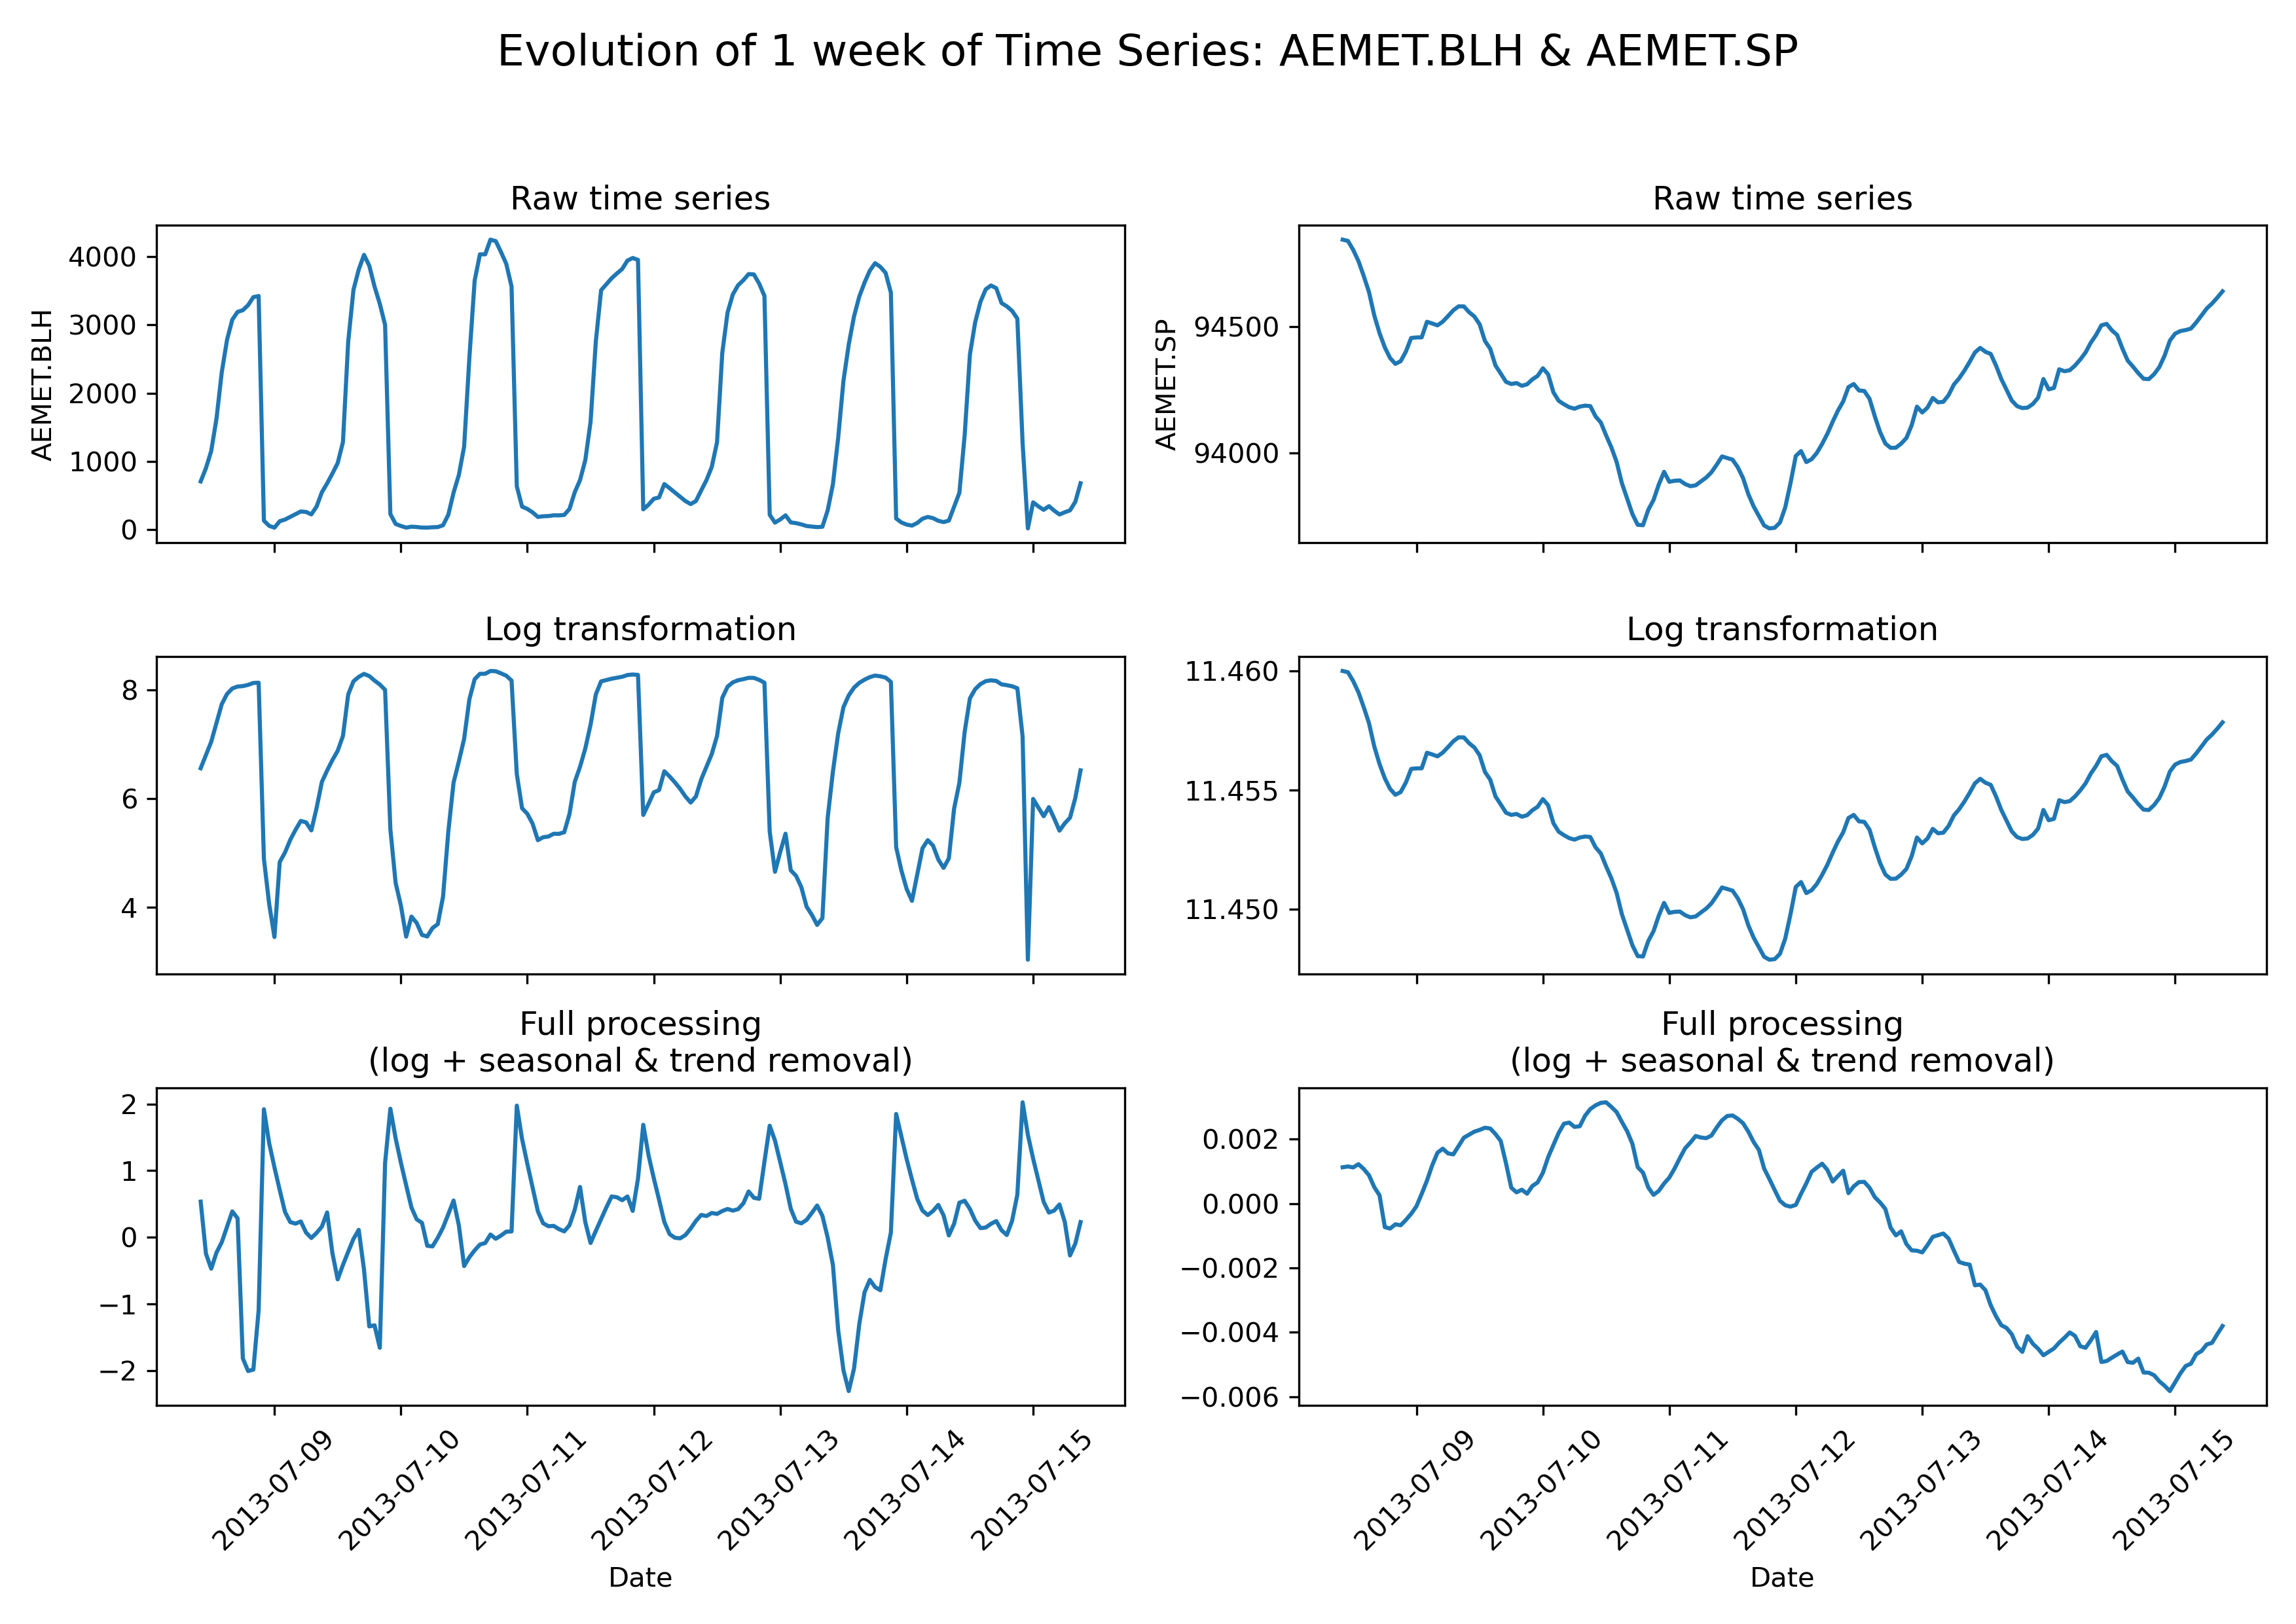
\includegraphics[width=\textwidth]{time_series_page_1.png}
  \caption{Time series used as input training data (raw form, after log transformation, and after full pre-processing which removes trend and seasonal components). Data sources described in \ref{data:sources}.}
  \label{fig:evo_ts1}
\end{figure}

\begin{figure}[h]
  \centering  
  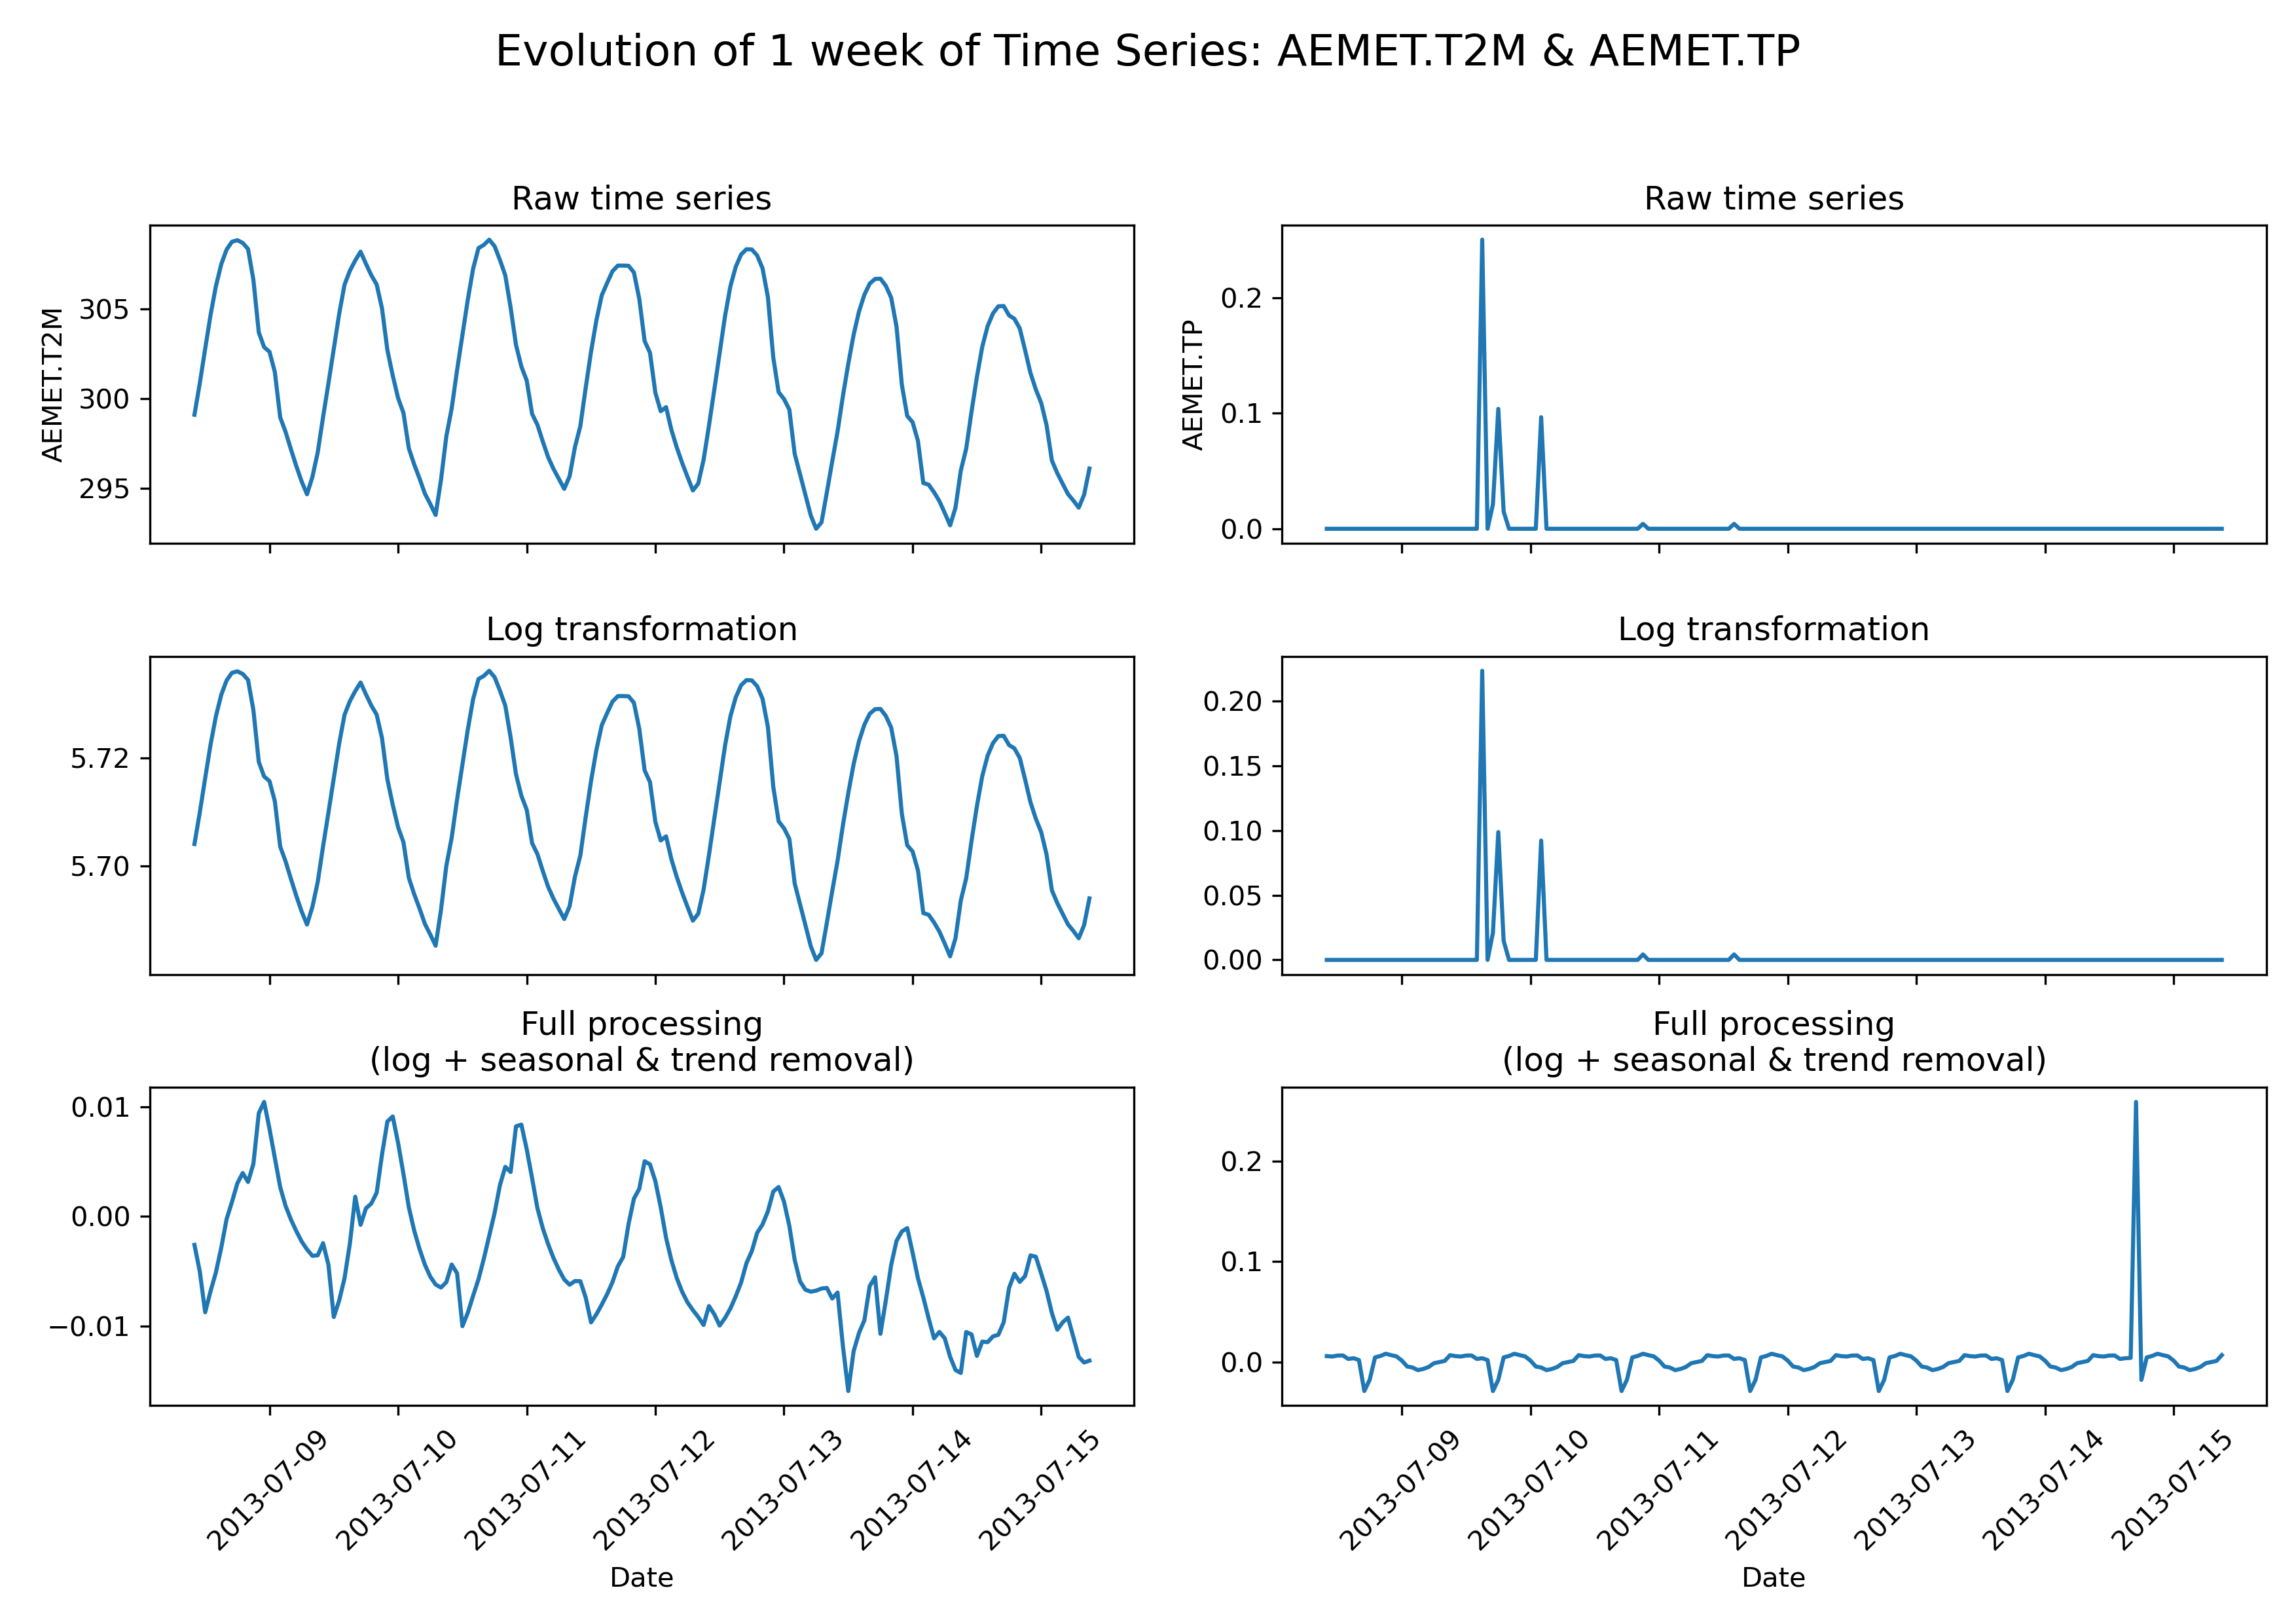
\includegraphics[width=\textwidth]{time_series_page_2.png}
  \caption{Time series used as input training data (raw form, after log transformation, and after full pre-processing which removes trend and seasonal components). Data sources described in \ref{data:sources}.}
  \label{fig:evo_ts2}
\end{figure}

\begin{figure}[h]
  \centering  
  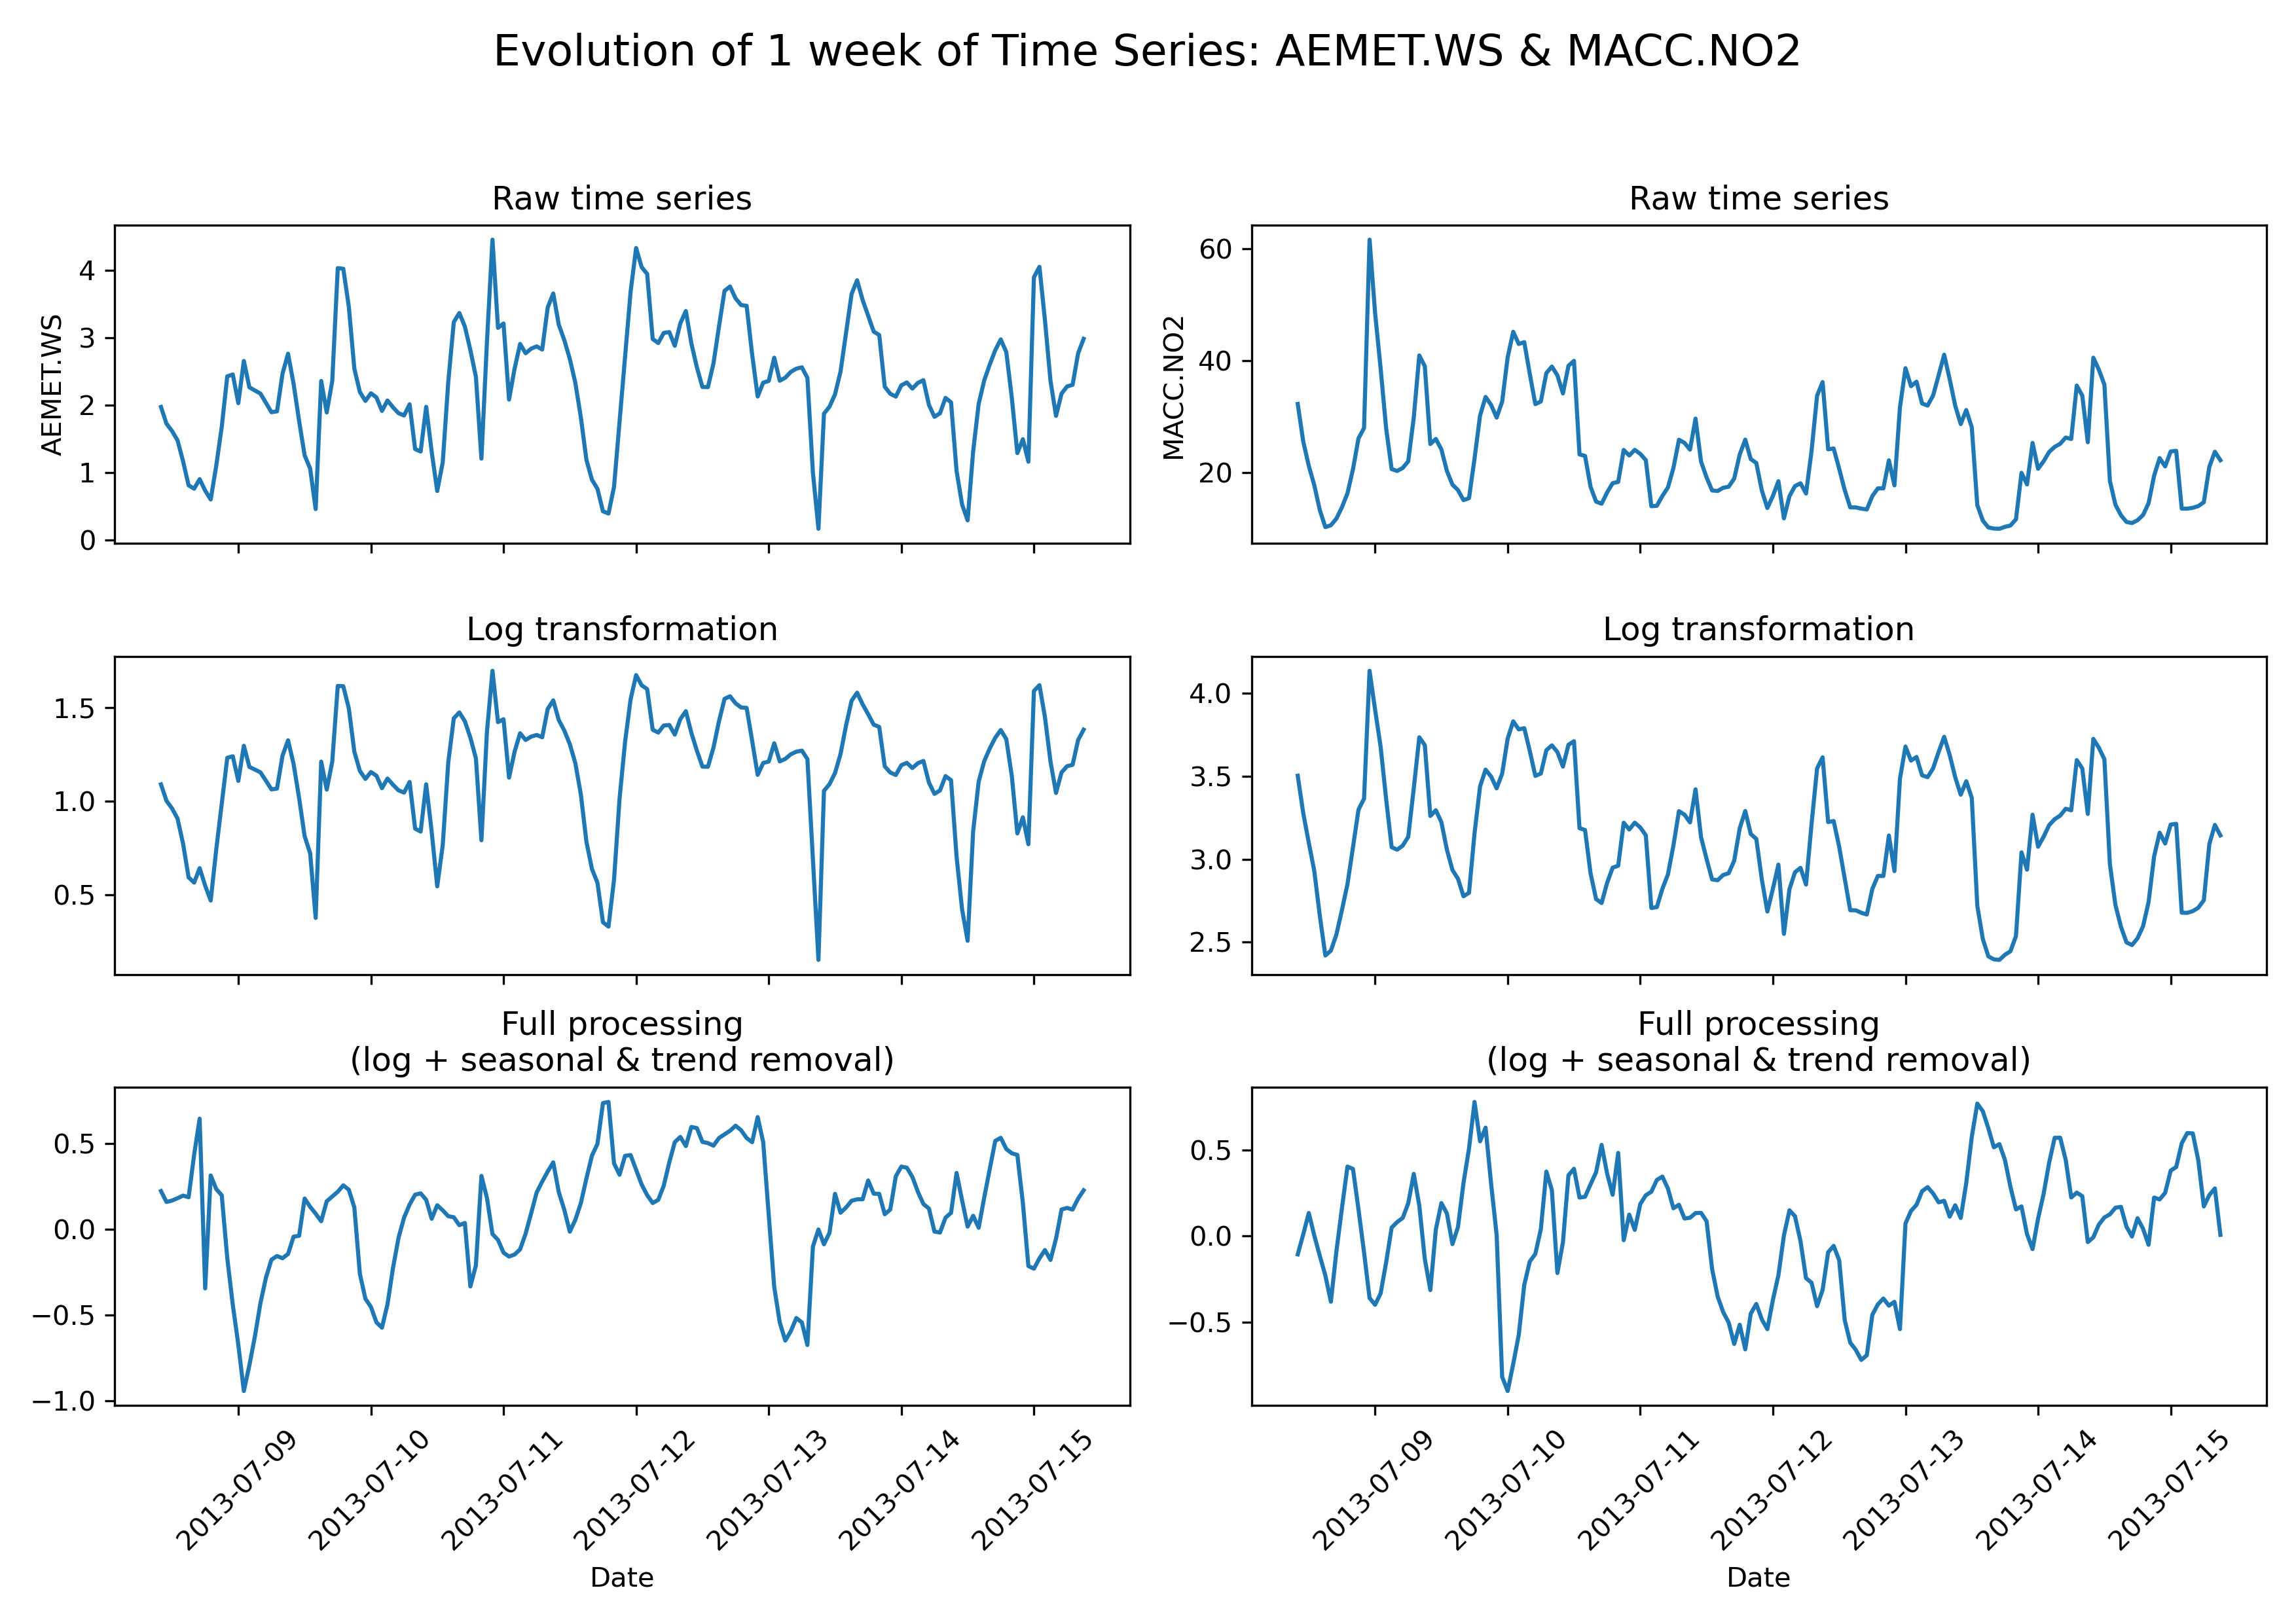
\includegraphics[width=\textwidth]{time_series_page_3.png}
  \caption{Time series used as input training data (raw form, after log transformation, and after full pre-processing which removes trend and seasonal components). Data sources described in \ref{data:sources}.}
  \label{fig:evo_ts3}
\end{figure}

\begin{figure}[h]
  \centering  
  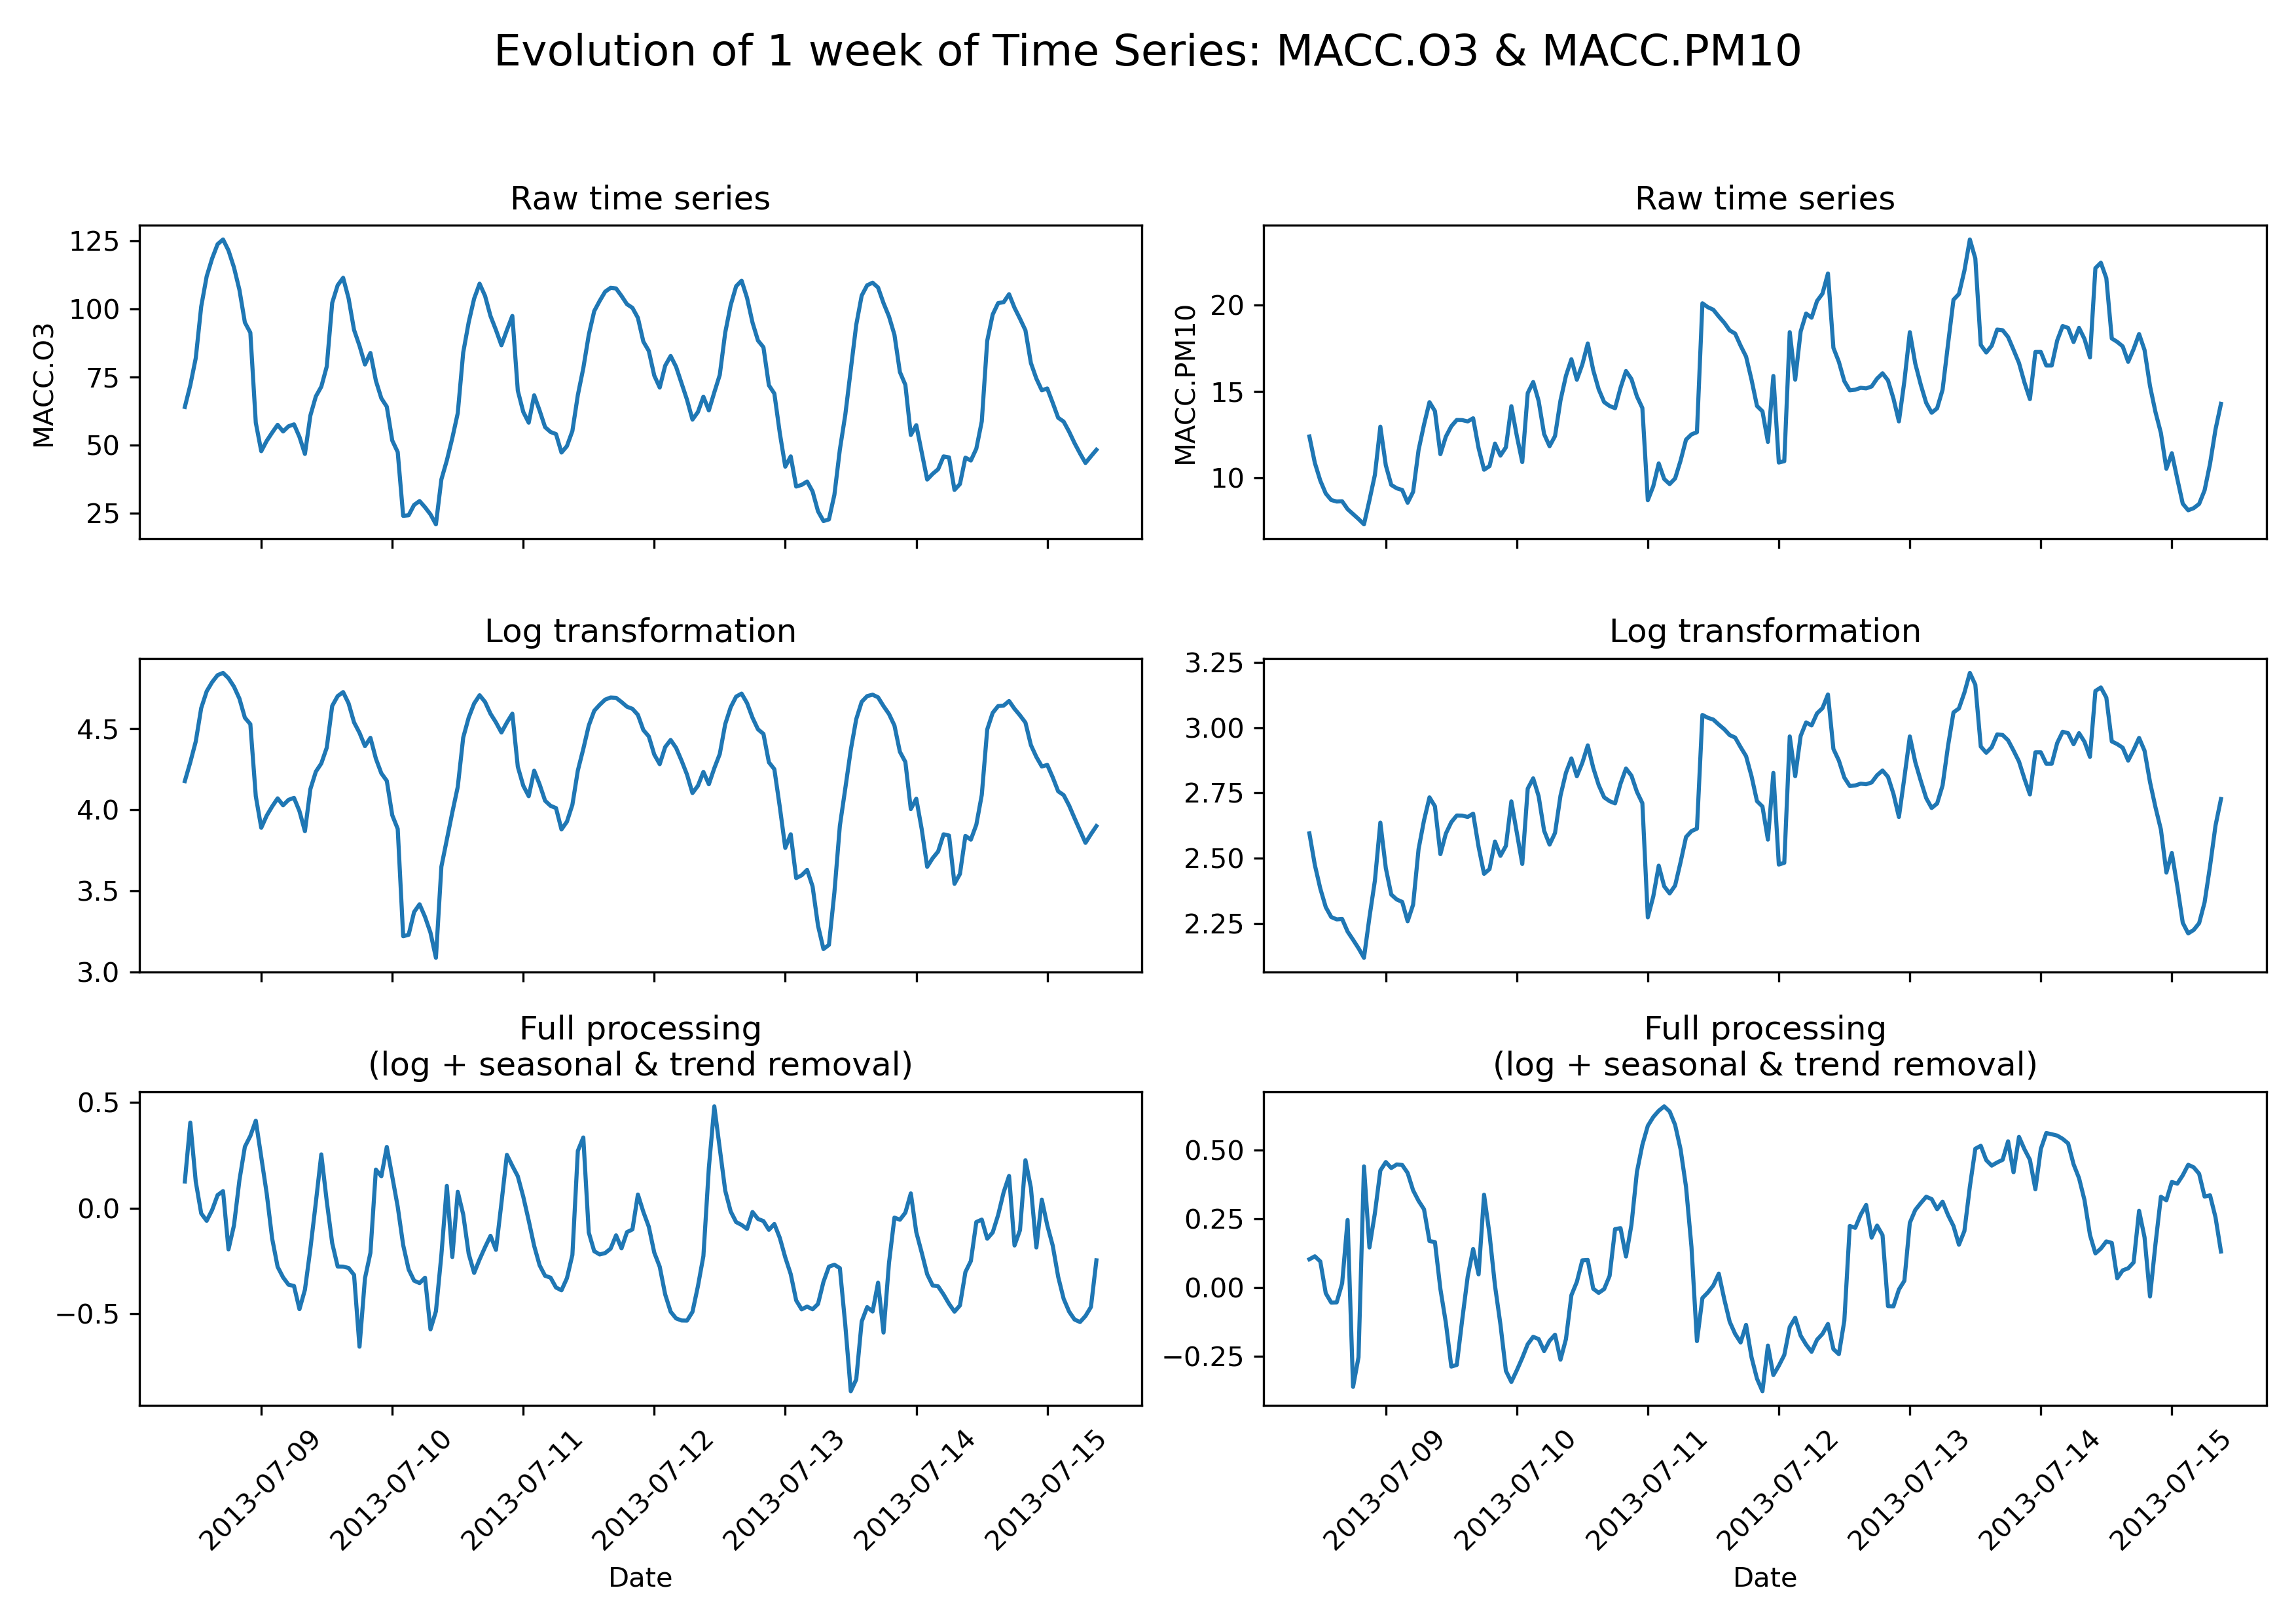
\includegraphics[width=\textwidth]{time_series_page_4.png}
  \caption{Time series used as input training data (raw form, after log transformation, and after full pre-processing which removes trend and seasonal components). Data sources described in \ref{data:sources}.}
  \label{fig:evo_ts4}
\end{figure}

\begin{figure}[h]
  \centering  
  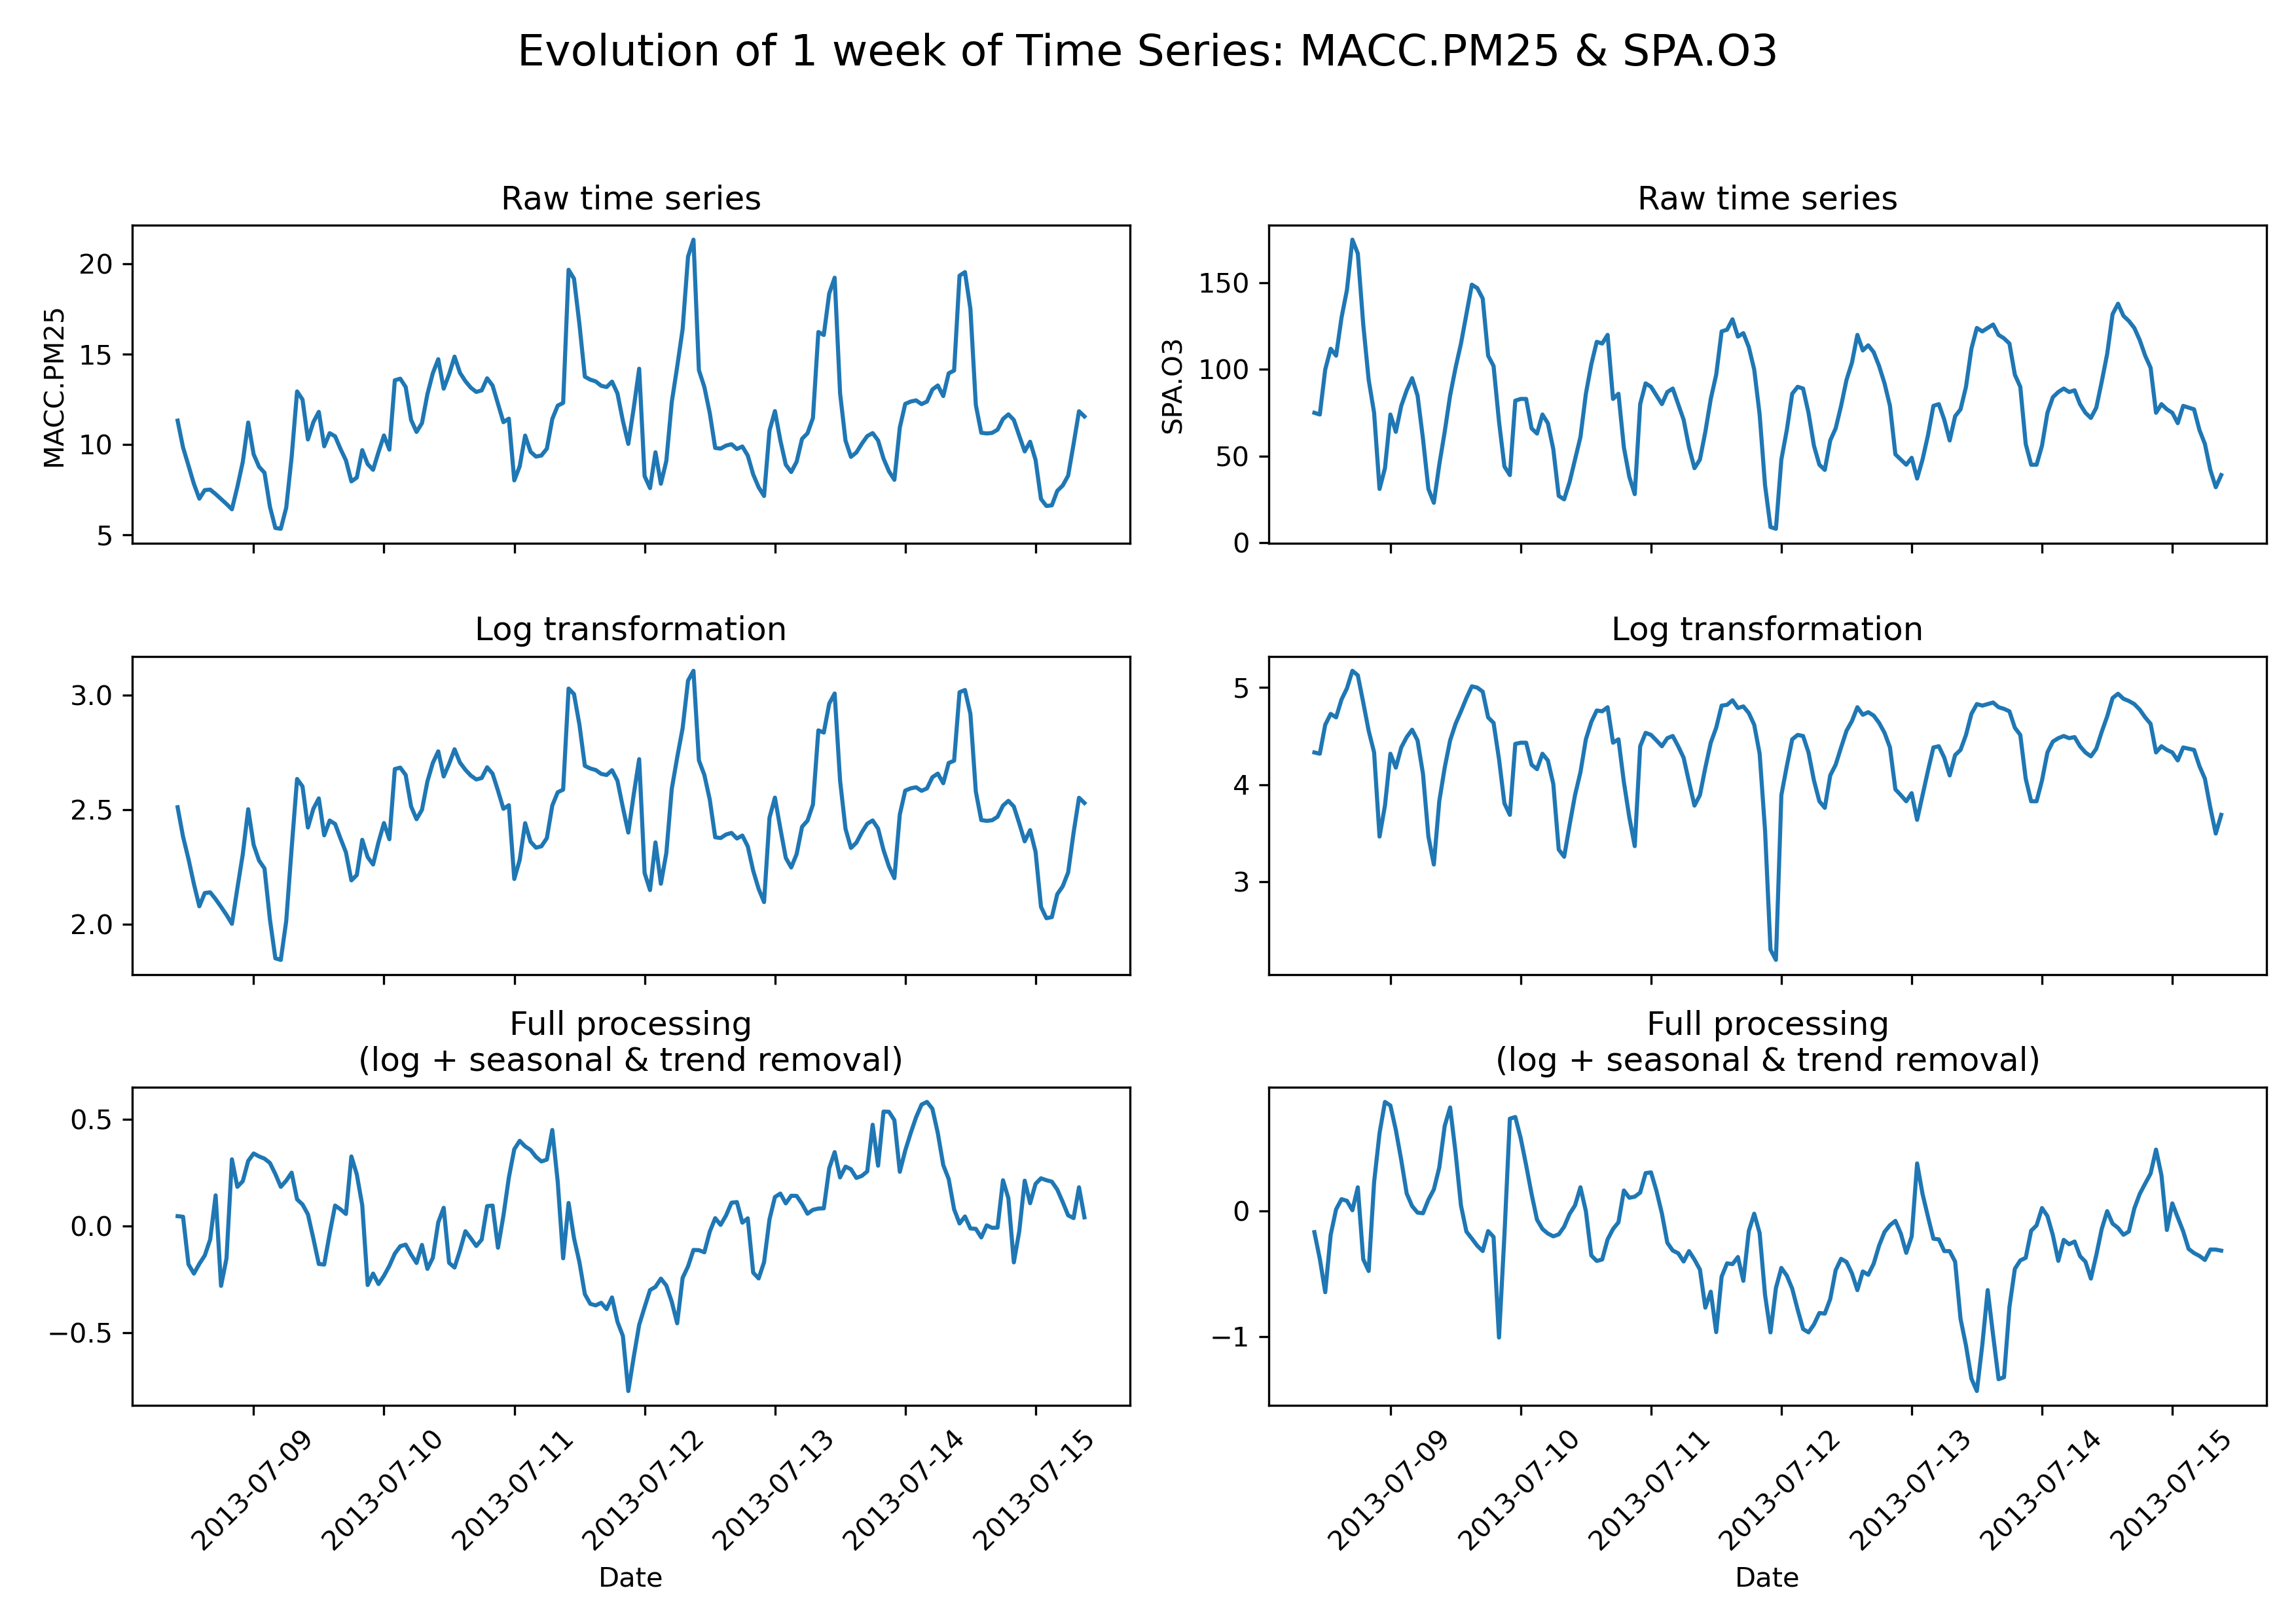
\includegraphics[width=\textwidth]{time_series_page_5.png}
  \caption{Time series used as input training data (raw form, after log transformation, and after full pre-processing which removes trend and seasonal components). Data sources described in \ref{data:sources}.}
  \label{fig:evo_ts5}
\end{figure}

\begin{figure}[h]
  \centering  
  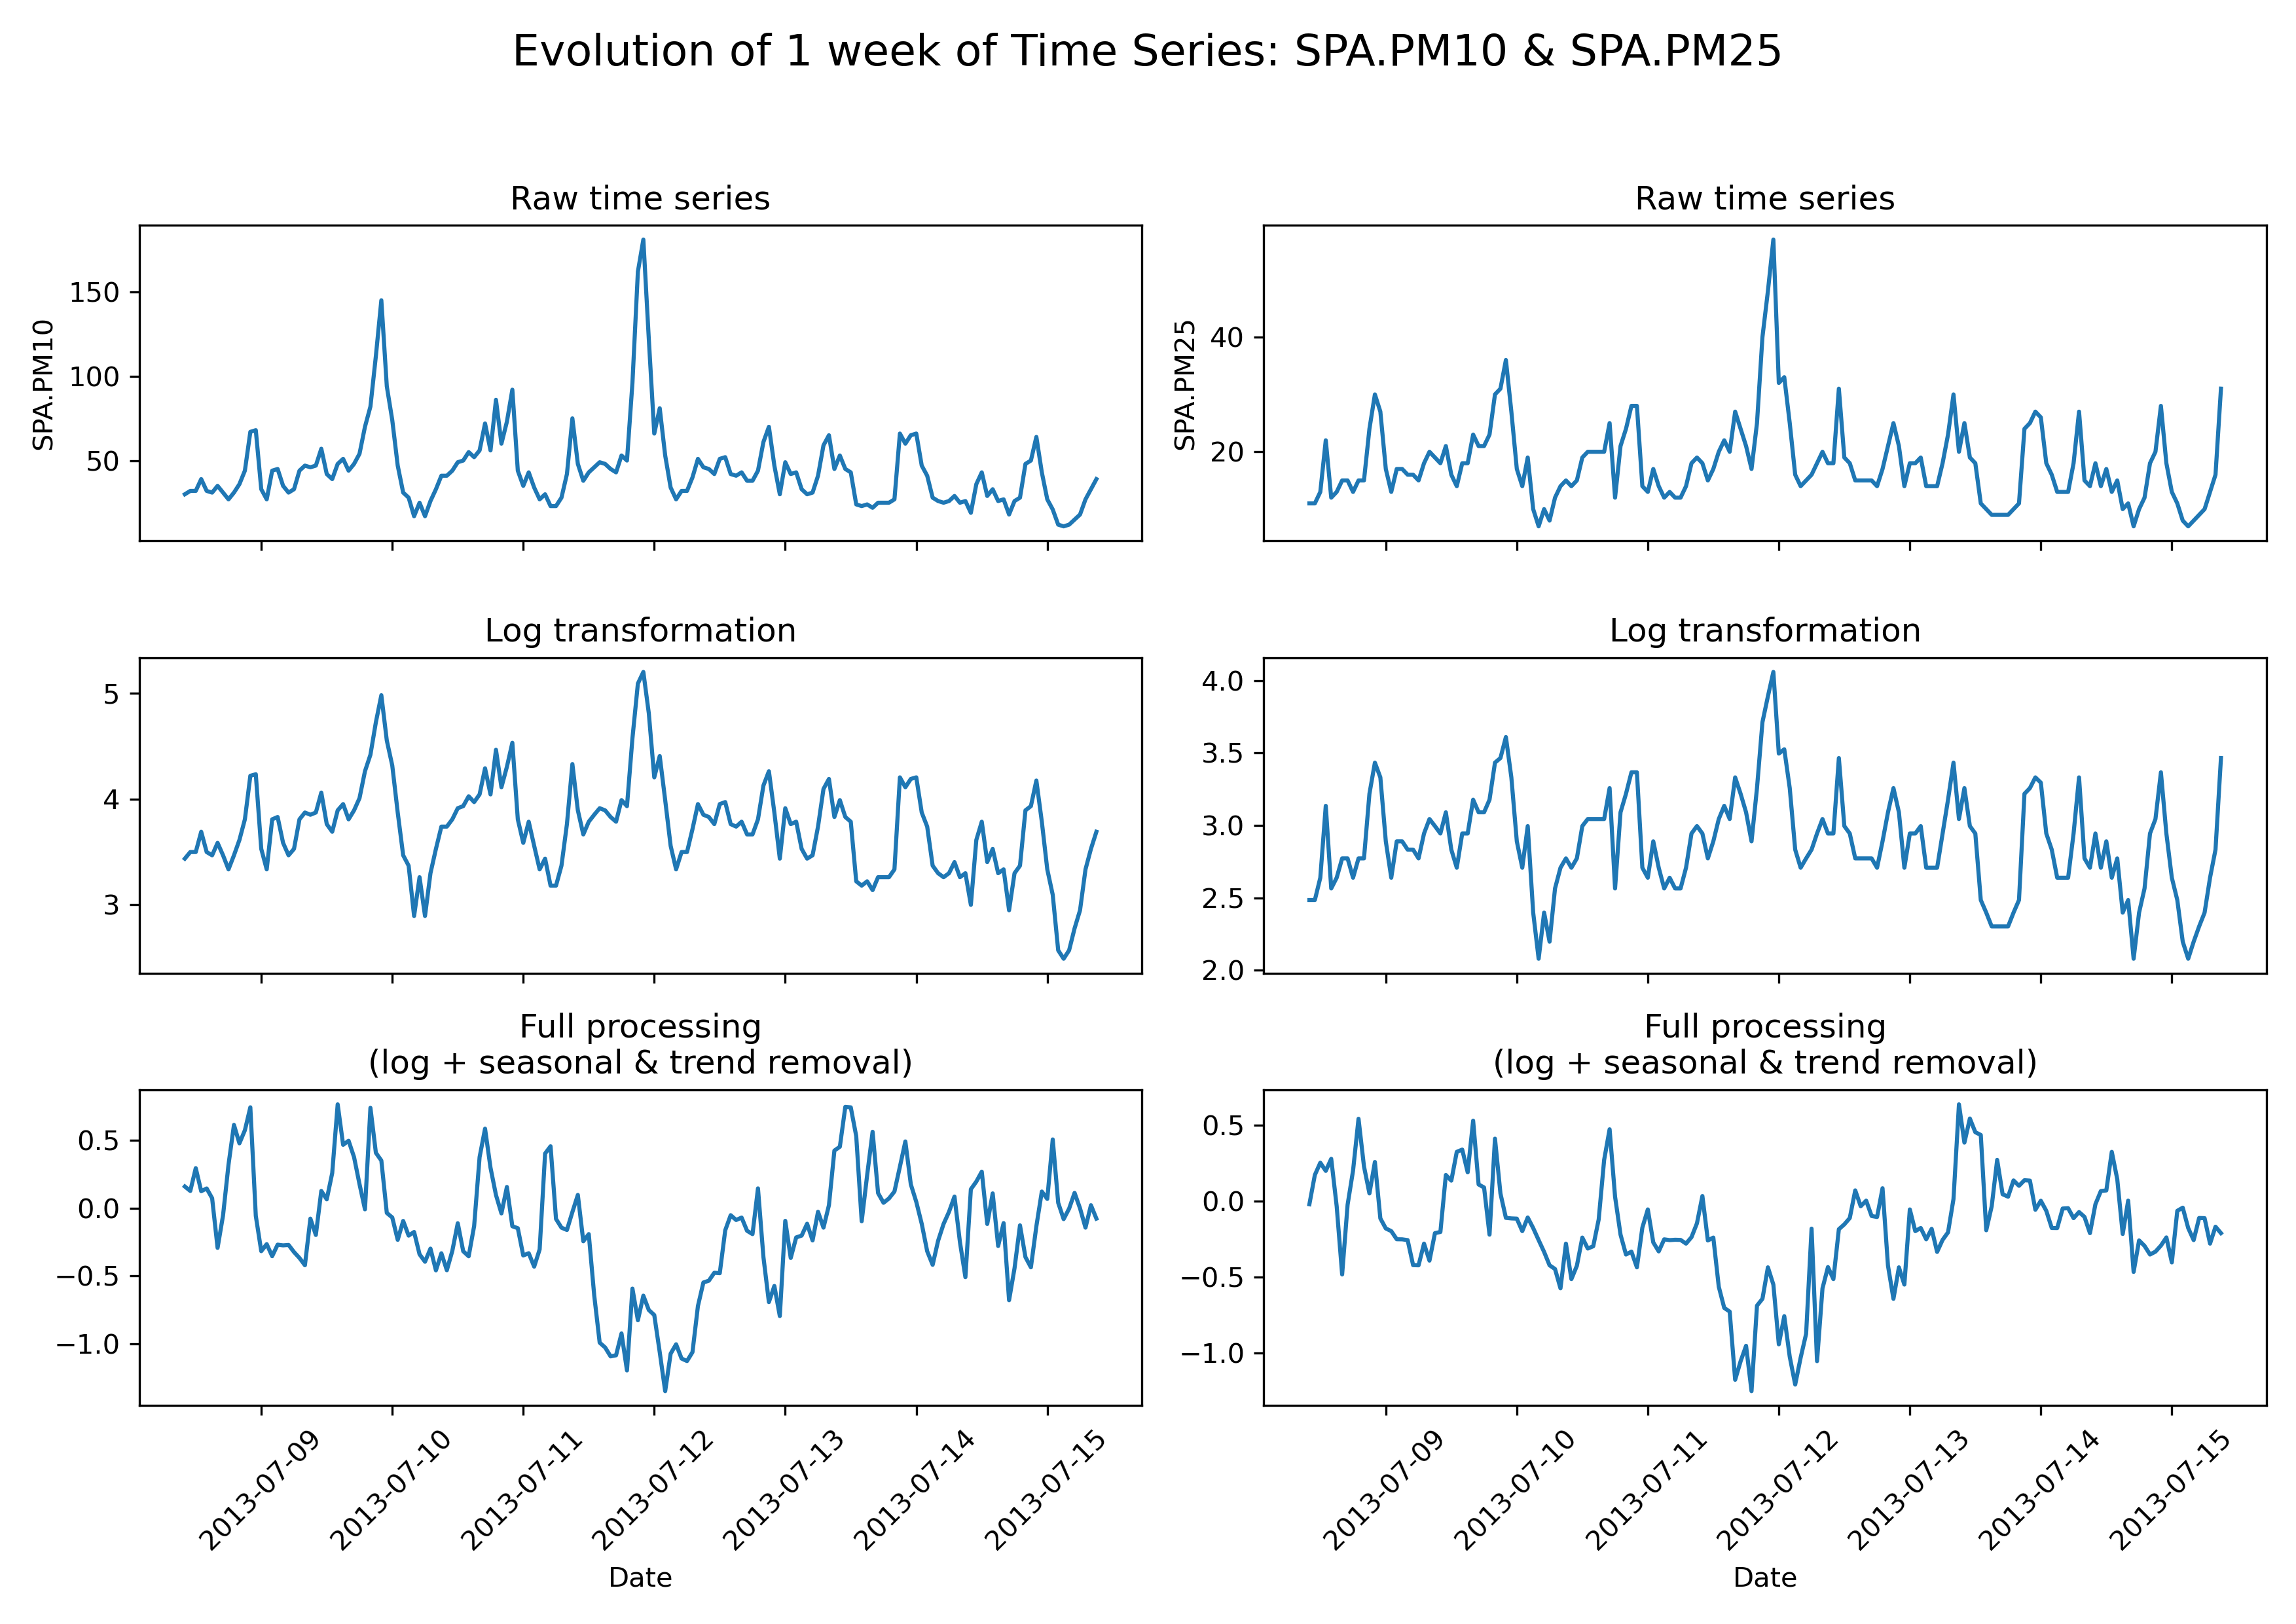
\includegraphics[width=\textwidth]{time_series_page_6.png}
  \caption{Time series used as input training data (raw form, after log transformation, and after full pre-processing which removes trend and seasonal components). Data sources described in \ref{data:sources}.}
  \label{fig:evo_ts6}
\end{figure}

\begin{figure}[h]
  \centering  
  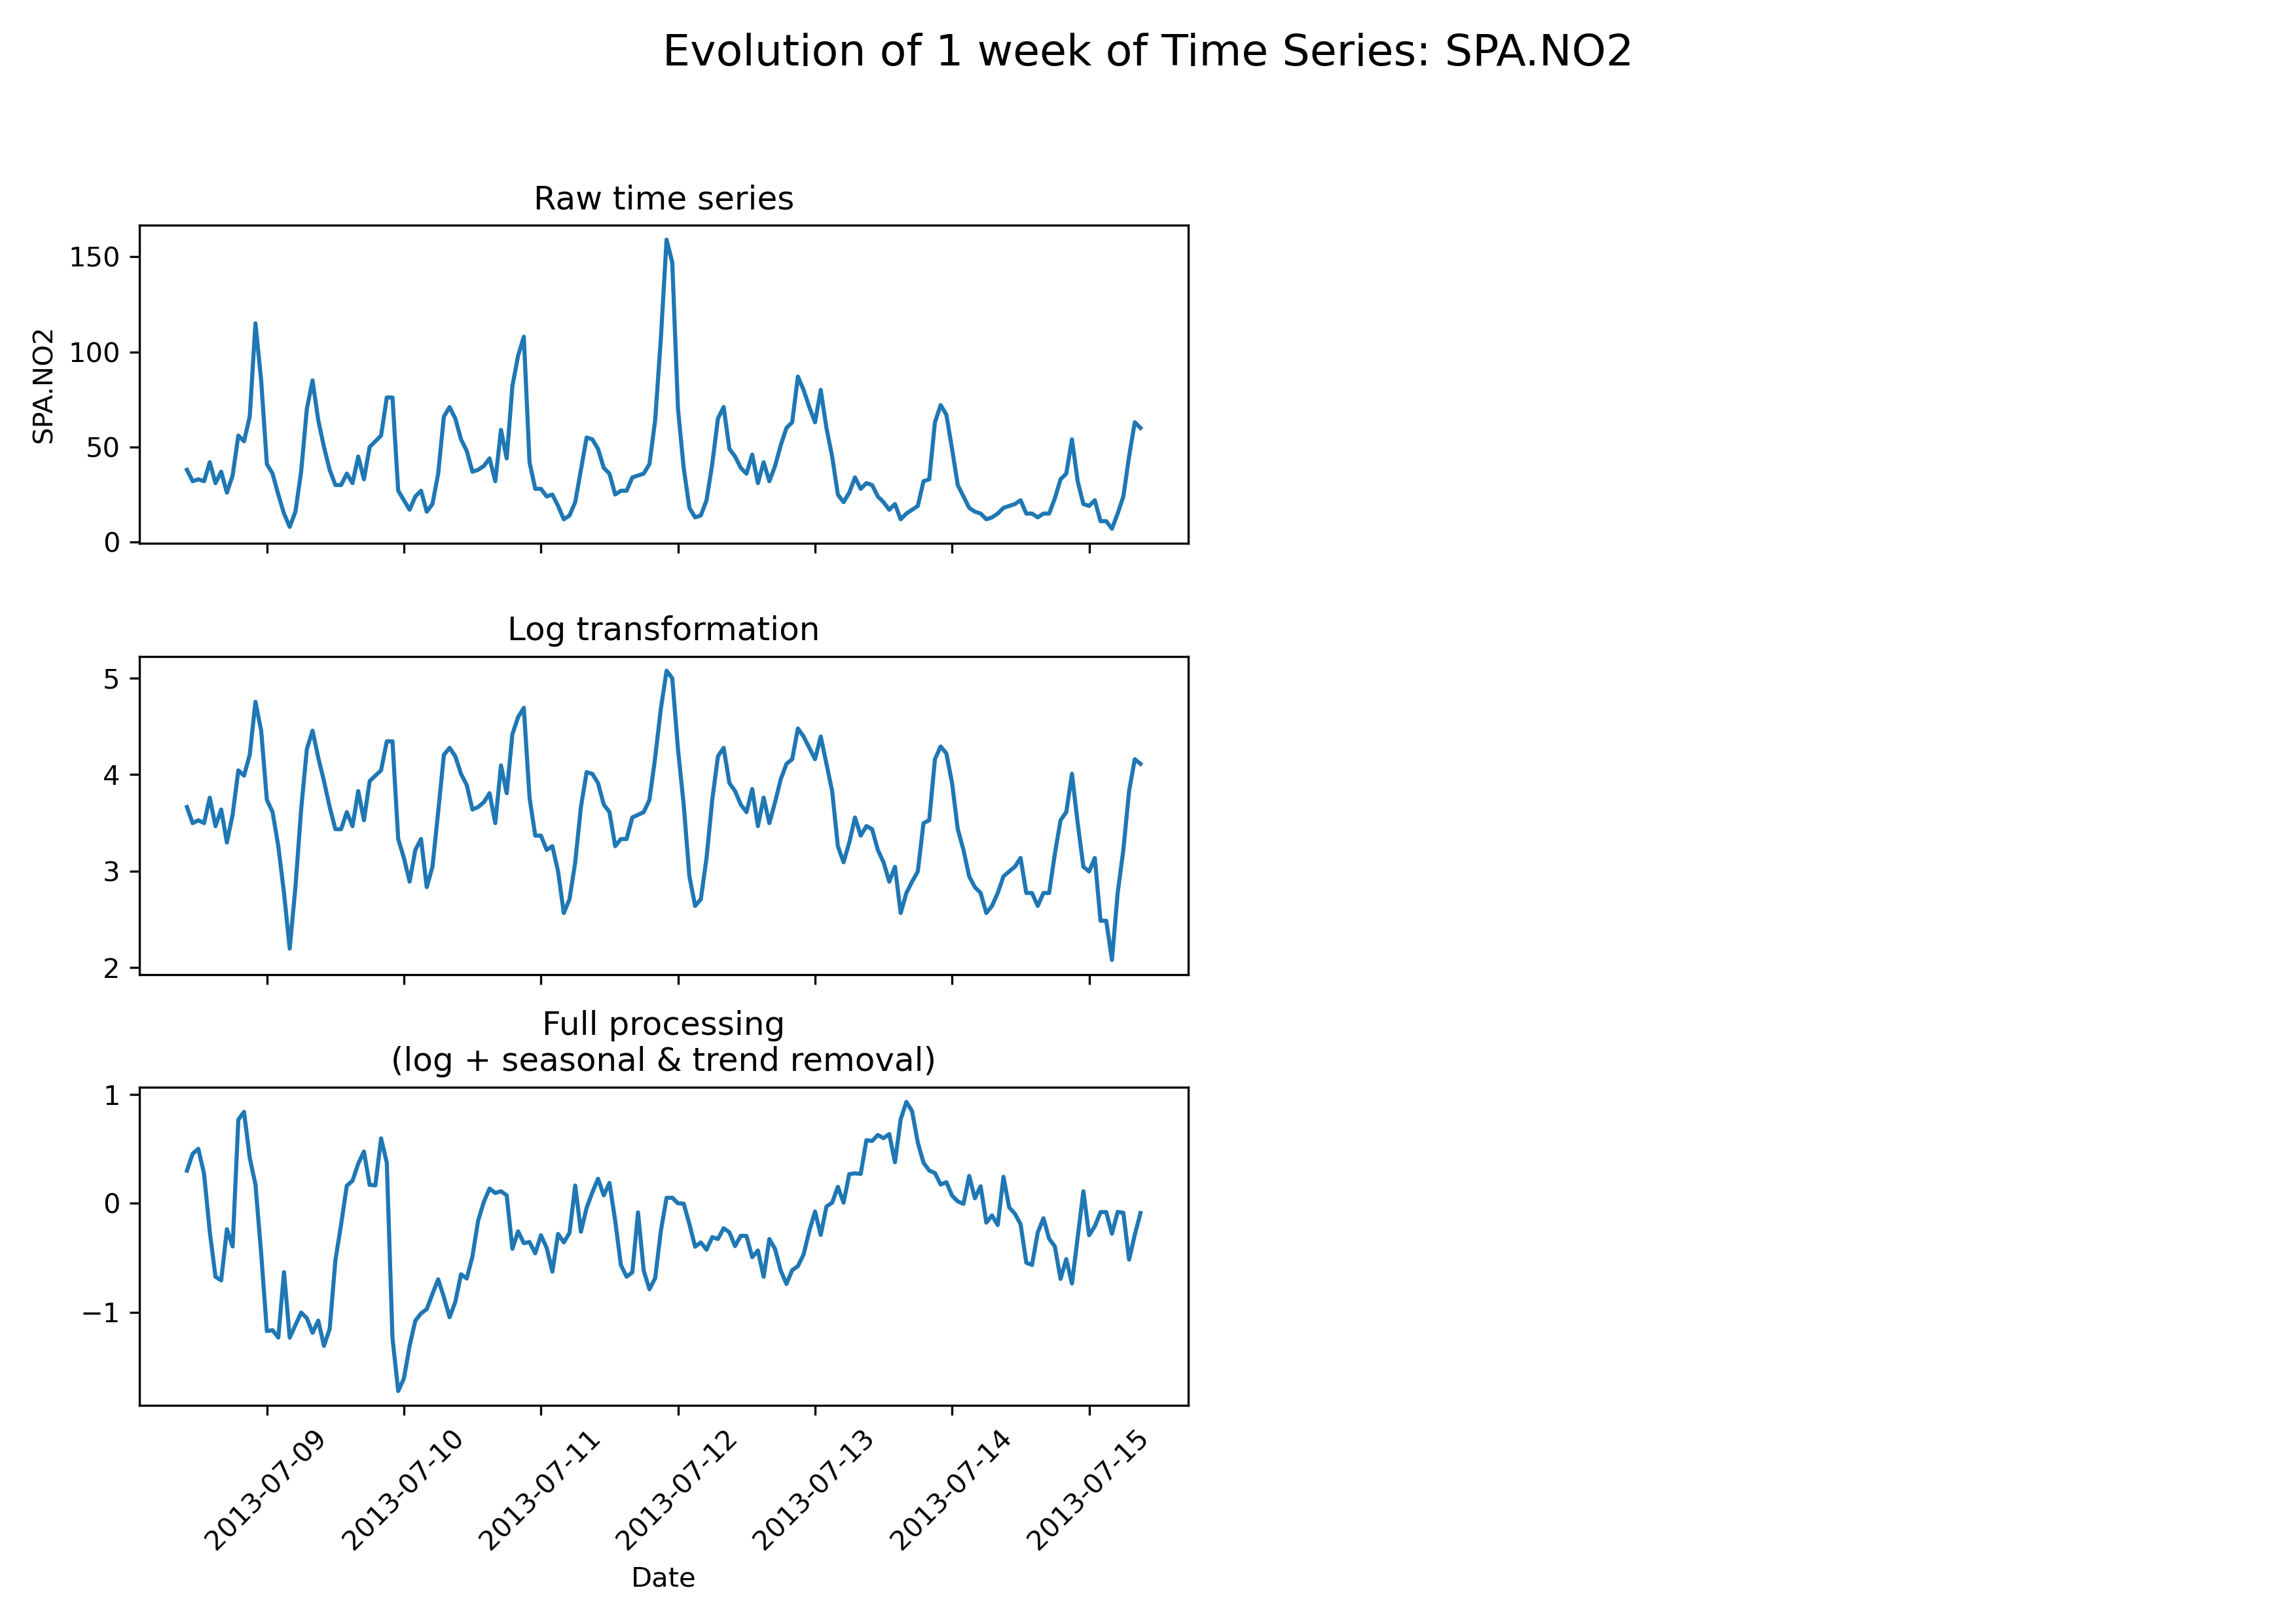
\includegraphics[width=\textwidth]{time_series_page_7.png}
  \caption{Time series used as input training data (raw form, after log transformation, and after full pre-processing which removes trend and seasonal components). Data sources described in \ref{data:sources}.}
  \label{fig:evo_ts7}
\end{figure}





\end{document}
